\documentclass[12pt]{report}

\usepackage{Dedman-Thesis-Latex-Template/sty/DL_thesis}  % Global Style for particular SMU College, e.g. DL_thesis.sty

\input{Dedman-Thesis-Latex-Template/latex/packages.tex}
% Load additional packages here.
% Be careful of the loading order with respect to packages.tex as conflicts can easily arise.
% This is not a part of the base template and so will never be overwritten during updates.
\usepackage{slashed}% https://www.ctan.org/pkg/slashed
\usepackage{braket}% https://www.ctan.org/pkg/braket
 % Uncomment to load additional user required packages
\input{Dedman-Thesis-Latex-Template/latex/preamble.tex}

\input{Dedman-Thesis-Latex-Template/latex/custom_commands.tex}
% Place your own personal commands here.
% This is not a part of the base template and so will never be overwritten during updates.

% Units
\newcommand{\eV}{\mathrm{eV}}% eV
\newcommand{\MeV}{\mathrm{MeV}}% MeV
\newcommand{\GeV}{\mathrm{GeV}}% GeV
\newcommand{\TeV}{\mathrm{TeV}}% TeV

% Physics processes
\newcommand{\Zbb}{Z \to b\bar{b}}% Z to bb
\newcommand{\Hbb}{H \to b\bar{b}}% Higgs to bb
\newcommand{\Xbb}{X \to b\bar{b}}% X to bb
\newcommand{\jXbb}{j + \Xbb}% X to bb with associated jet
 % Uncomment to use your own personal commands
\AuthorFirstName{Matthew}
\AuthorLastName{Feickert}

% Title can be up to three lines of no more than 48 characters per line
\ThesisTitle{A Search for Higgs Bosons decaying to the $\MakeLowercase{b}\bar{\MakeLowercase{b}}$ Final State}{Through Production with An Initial State Radiation Jet}{using the ATLAS Detector at $\sqrt{\MakeLowercase{s}}=\SI{13}{\tera\electronvolt}$}
\GraduateDepartment{Physics}

\FirstDegree%
\FirstDegreeType{B.S.}
\FirstDegreeMajor{Physics}
\FirstDegreeUniversity{Undergraduate University}

\SecondDegree%
\SecondDegreeType{M.A.}
\SecondDegreeMajor{Physics}
\SecondDegreeUniversity{University of Virginia}

\ThirdDegree%
\ThirdDegreeType{M.S.}
\ThirdDegreeMajor{Physics}
\ThirdDegreeUniversity{Southern Methodist University}

\ThesisDefenseDateYear{2019}
\ThesisDefenseDateMonth{April}
\ThesisDefenseDateDay{17}

\GraduationDateYear{2019}
\GraduationDateMonth{May}
\GraduationDateDay{14}

\SMUCollege{Dedman College}

% Committee
\AdvisorFullName{Dr.~Stephen Sekula}
\AdvisorTitle{Associate Professor}

\CommitteeMemberA{Dr.~Jingbo Ye}
\CommitteeMemberTitleA{Professor}

\CommitteeMemberB{Dr.~Roberto Vega}
\CommitteeMemberTitleB{Associate Professor}

\CommitteeMemberC{Dr.~TBA}
\CommitteeMemberTitleC{Assistant Professor}

\input{latex/metadata.tex}

\makeglossaries
\newglossaryentry{LHC}{
 name=LHC,
 description={Large Hadron Collider}
}

\newglossaryentry{interaction point}{
 name=interaction point,
 description={Point along the LHC where the LHC beams can be brought into crossing for collisions}
}

\newglossaryentry{Pseudorapidity}{
 name=pseudorapidity,
 description={High energy approximation of the rapidity that only requires angular information}
}

\newglossaryentry{rapidity}{
 name=rapidity,
 description={A measurement of the speed of a particle along a given axis given its energy and total momentum}
}

\newglossaryentry{Lorentz invariant}{
 name=Lorentz invariant,
 description={A scalar value quantity that is invariant under a Lorentz transformation, such as a spacetime interval or the mass of a particle},
 text=Lorentz invariant,
 plural=Lorentz invariants
}

\newglossaryentry{boost}{
 name=Lorentz boost,
 description={A Lorentz transformation without any rotations, such that the reference frame is ``boosted'' along a single direction},
 text=boost,
 plural=boosts
}

\newglossaryentry{Proton Synchrotron}{
 name=Proton Synchrotron,
 description={Synchrotron accelerator in the LHC injection chain where the proton beams form a bunch train with $25~\textrm{ns}$ spacing}
}

\newglossaryentry{ATLAS}{
 name=ATLAS,
 description={a general-purpose detector at the \Gls{LHC}}
}

\newglossaryentry{Standard Model}{
 name=Standard Model,
 description={}
}

\newglossaryentry{dark matter mediator}{
 name=dark matter mediator,
 description={massive exotic particle with couplings to both Standard Model particles and dark matter}
}

\newglossaryentry{MCMC}{
 name=MCMC,
 description={Markov Chain Monte Carlo}
}


\thesisdraft % uncomment if want draft printing

\begin{document}

\input{Dedman-Thesis-Latex-Template/latex/front_pages.tex}

\begin{thesis}

 \chapter*{Preface}\label{chapter:preface}
% c.f. https://tex.stackexchange.com/a/222961/152544
\addcontentsline{toc}{chapter}{\protect\numberline{}Preface}

The following is a summary of useful concepts in high energy particle physics.

\section{Units}\label{section:units}

\subsection{Natural Units}\label{subsection:natural_units}

The nature of high energy physics is to give descriptions of the phenomena and interactions that occur at energies that result in speeds that are close to the speed of light over very short time and distance scales.
Given this, it becomes readily apparent that International System of Units (SI) of measurement are somewhat cumbersome to use in calculations, and a much more useful system of units would be consistent with the scale of the phenomena.
When measuring the speed of a relativistic particle it is more convenient to compare to the speed of light $\left(\text{such that }c=1\right)$ then to the number of meters per second.
Similarly, when measuring the momentum of a particle it is generally more useful to know the amount of its energy in the form of momentum compared to the amount in the form of its mass, resulting in expressing momentum in terms of energy.
This system of units is called ``Natural Units'', and builds its measurements in terms of speed, angular momentum, and energy.
It is used extensively (if not almost exclusively) throughout high energy physics.
Quantities encountered routinely in high energy physics are given in Natural Units in \Cref{table:natural_units}.
\TODO{Describe cross section.}

\begin{table}[htpb]
 \centering
 \caption{Common quantities in particle physics given in both natural units and SI units.}
 \begin{tabular}{@{}llll@{}} \toprule
  Quantity         & Natural Units                 & Natural Units (dimensionful)            & SI Units                                              \\ \midrule
  Speed            & $1$                           & $c$                                     & $3.0\times 10^{8}~\mathrm{m}/\mathrm{s}$              \\
  Angular Momentum & $1$                           & $\hbar$                                 & $10^{34}~\mathrm{m}^2 \,\mathrm{kg}/\mathrm{s}$       \\
  Energy           & $\mathrm{GeV}$                & $\mathrm{GeV}$                          & $1.6\times 10^{-10}~\mathrm{J}$                       \\
  Momentum         & $\mathrm{GeV}$                & $\mathrm{GeV}/c$                        & $1\times 10^{-19}~\mathrm{kg}\,\mathrm{m}/\mathrm{s}$ \\
  Mass             & $\mathrm{GeV}$                & $\mathrm{GeV}/c^{2}$                    & $1.8\times 10^{-27}~\mathrm{kg}$                      \\
  Time             & $1/\mathrm{GeV}$              & $\hbar/\mathrm{GeV}$                    & $6.6\time 10^{-25}~\mathrm{s}$                        \\
  Length           & $1/\mathrm{GeV}$              & $\hbar c/\mathrm{GeV}$                  & $2\times 10^{-16}~\mathrm{m}$                         \\
  Electric Charge  & $1$                           & $e/\sqrt{4\pi \alpha_{\mathrm{em}}}$    & $5.3\times 10^{-19}~\mathrm{C}$                       \\
  Magnetic Field   & $\left(\mathrm{GeV}\right)^2$ & $\left(\mathrm{GeV}\right)^2/\hbar c^2$ & $5\times 10^{16}~\mathrm{T}$                          \\
  \bottomrule
 \end{tabular}\label{table:natural_units}%
\end{table}


\subsection{Units of Luminosity}\label{subsection:luminosity_units}
In high energy physics a crucial quantity of interest is the luminosity (both instantaneous and integrated) delivered by the particle accelerator.
The instantaneous luminosity, $\mathscr{L}$, can be defined as the number of particles incident per unit area per unit time (generally taken to be seconds),
\begin{equation}
 \mathscr{L} = \frac{\text{number of particles}}{\text{unit area} \cdot \text{second}}.
 \label{eq:instantaneous_luminosity}
\end{equation}
In accelerator physics, the unit area is generally chosen to be $\textrm{cm}^2$, giving instantaneous luminosities units of $\textrm{cm}^{-2} \cdot \textrm{s}^{-1}$,
\[
 \left[\mathscr{L}\right] = \textrm{cm}^{-2} \cdot \textrm{s}^{-1}.
\]
However, experimental particle physicists prefer to use units of inverse barns for luminosities. A barn is defined as
\begin{equation}
 1~\textrm{barn} = 10^{-28}~\textrm{m}^2 = 10^{-24}~\textrm{cm}^2,
 \label{eq:barn_to_area}
\end{equation}
which is roughly the cross sectional area of an atomic nuclei~\cite{web:history_physics_purdue,history:etymology_barn}.

The context in which luminosity appears as being useful is in the form of an equation like
\begin{equation}
 N_{\textrm{events}} = \sigma_{\textrm{process}} \cdot \int \mathscr{L}\,dt
 \label{eq:events_from_luminosity}
\end{equation}
where:
\begin{itemize}
 \item $N_{\text{events}}$ is the number of events of a particular process that will be produced at the collider.
       This is what ends up exiting the collision process.
 \item $\sigma_{\textrm{process}}$ is the cross section of the particular process to occur per interaction of colliding particles.
       At the \Gls{LHC} this would be the cross section per proton-proton interaction.
       This is a function of the fundamental physics that is available at the energy ranges being probed, and so is also a function of the collider's center of mass energy, $\sqrt{s}$.
       When written in an equation as such it is assumed that the cross section is also including the relevant branching ratios for the final state particles.
       That is, $\sigma\left(pp \to H \to b\bar{b}\,\right) = \sigma\left(pp \to H\right) \cdot \mathcal{BR}\left(H \to b\bar{b}\,\right)$.
 \item $L \equiv \int \mathscr{L}\,dt$ is the total luminosity integrated over time (the integrated luminosity).~\cite{Herr:941318}
       This is what is delivered by the particle accelerator.
\end{itemize}

\begin{table}[htpb]
 \centering
 \caption{Instantaneous luminosities at the LHC.}
 \begin{tabular}{@{}ll@{}} \toprule
  Description                                                    & Units of $\textrm{cm}^{-2}\cdot\textrm{s}^{-1}$ \\ \midrule
  LHC Design Luminosity~\cite{Bruning:782076}                    & $10^{34}$                                       \\
  2017 ATLAS Trigger Menu Maximum~\cite{TWiki:MenuEvolution2017} & $2.0 \times 10^{34}$                            \\
  2017 Plan~\cite{Indico:MenuCoordination_2017Lumi}              & $1.7 \times 10^{34}$                            \\
  2017 Peak~\cite{TWiki:2017ATLASPeakLumi}                       & $2.09 \times 10^{34}$                           \\
  2018 Peak~\cite{TWiki:2018ATLASPeakLumi}                       & $2.1 \times 10^{34}$                            \\
  \bottomrule
 \end{tabular}\label{table:LHC_Luminosity_Goals}%
\end{table}

% Note to self: spacing in tables seems too large. See if can adjust with geometry package
\begin{table}[htpb]
 \centering
 \caption{Luminosity measurements in $\text{barns}^{-1}$.}
 % \resizebox{\linewidth}{!}{%
 % \resizebox*{!}{\dimexpr\textheight-2\baselineskip\relax}{%
 \begin{tabular}{@{}lll@{}} \toprule
  Units                & Units of $\textrm{cm}^{-2}$ & Units of $\textrm{fb}^{-1}$ \\ \midrule
  $\textrm{barn}^{-1}$ & $10^{24}$                   & $10^{-15}$                  \\
  $\textrm{mb}^{-1}$   & $10^{27}$                   & $10^{-12}$                  \\
  $\mu\textrm{b}^{-1}$ & $10^{30}$                   & $10^{-9}$                   \\
  $\textrm{nb}^{-1}$   & $10^{33}$                   & $10^{-6}$                   \\
  $\textrm{pb}^{-1}$   & $10^{36}$                   & $10^{-3}$                   \\
  $\textrm{fb}^{-1}$   & $10^{39}$                   & $10^{0}$                    \\
  $\textrm{ab}^{-1}$   & $10^{42}$                   & $10^{3}$                    \\
  \bottomrule
 \end{tabular}\label{table:Luminosity}%
 % }
\end{table}

\section{Coordinates}\label{section:coordinates}

The LHC coordinate system, seen in \Cref{fig:LHC_coordinate_system}, is a rectangular coordinate system defined relative to the LHC ring and the LHC beamline.
At any point, the positive $x$ direction is defined as the direction that points radially inward to the center of the LHC ring.
The positive $y$ direction is then defined as pointing upwards --- radially outward from the center of the Earth --- leaving the positive $z$ direction pointing along the beamline.

\begin{figure}[htbp]
 \centering
 \includegraphics[width=0.8\linewidth]{preface/LHC_coordinate_system.pdf}
 \caption{The LHC coordinate system as seen from the ATLAS detector.}
 \label{fig:LHC_coordinate_system}
\end{figure}

While the LHC coordinate system is Cartesian, the preferred coordinate system for describing LHC events is not.
As the ATLAS detector is arranged cylindrically around the beamline of the LHC --- such that most of its detector components are transverse to the beamline --- the coordinate system that is used to describe events in ATLAS is characterized by a particle's transverse momentum, pseudorapidity, and azimuthal angle: $\left(p_T, \eta, \phi\right)$.
The polar angle, $\theta$, is defined as the angle relative to the beam axis, and the azimuthal angle, $\phi$, is measured around the beam axis.

\Gls{Pseudorapidity} is defined as
\begin{equation}
 \eta = - \ln \left(\tan \frac{\theta}{2}\right)
 \label{eq:pseudorapidity}
\end{equation}
to be a good approximation in the high energy regime of the \gls{rapidity} of a particle --- a measurement of the velocity of a particle longitudinal to the beam axis,
\begin{equation}
 y = \frac{1}{2} \ln \left(\frac{E + p_{z}}{E - p_{z}}\right).
 \label{eq:rapidity}
\end{equation}
As the beam axis is defined as $\hat{\vec{z}}$, such that $p_{z} = \abs{\vec{p}} \cos\theta$, then it is seen that in the relativistic limit, $\abs{\vec{p}} \gg m$, the rapidity reduces to the pseudorapidity
\[
 \begin{split}
  y   &\approx \frac{1}{2} \ln \left(\frac{p + p\cos\theta}{p - p\cos\theta}\right)\\
  &\approx \frac{1}{2} \ln \left(\frac{2 \cos^{2} \frac{\theta}{2}}{2 \sin^{2} \frac{\theta}{2}}\right) \\
  &\approx - \ln \left(\tan \frac{\theta}{2}\right) = \eta.
 \end{split}
\]
It is clear that the rapidity and the pseudorapidity are not \Glspl{Lorentz invariant}.
However, for a Lorentz \gls{boost} --- a Lorentz transformation without any rotations --- of speed $\beta$ along the beam axis, $\hat{\vec{z}}$,
\[
 \begin{pmatrix}
  E' \\
  p_{z}'
 \end{pmatrix}
 =
 \begin{pmatrix}%
  \gamma       & -\gamma\beta \\%
  -\gamma\beta & \gamma
 \end{pmatrix}%
 \begin{pmatrix}
  E \\
  p_{z}
 \end{pmatrix}\,,
\]
it is seen\footnote{Glossing over some algebra and hyperbolic trigonometric identities.} that the rapidity for a particle under the boost is the sum of the original rapidity and a constant of the boost
\[
 \begin{split}
  y'  &= \frac{1}{2} \ln \left(\frac{E' + p_{z}'}{E' - p_{z}'}\right) \\
  &= \frac{1}{2} \ln \left(\frac{E - \beta p_{z} + p_{z} - \beta E}{E - \beta p_{z} - p_{z} + \beta E}\right) \\
  &= \frac{1}{2} \ln \left(\frac{E + p_{z}}{E - p_{z}}\right) + \frac{1}{2} \ln \left(\frac{1 - \beta}{1 + \beta}\right) \\
  &= y - \tanh^{-1}\beta\,.
 \end{split}
\]
Thus, the \emph{difference in rapidities} between two particles is seen to be independent of the boost and so is a \Gls{Lorentz invariant}.
Defining the distance metric\footnote{$\Delta R$ is an angular distance in $\left(\eta, \phi\right)$ space, and can be thought of as a solid angle.} for two particles in $\left(\eta, \phi\right)$ space as
\begin{equation}
 \Delta R = \sqrt{\left(\Delta\eta\right)^{2} + \left(\Delta\phi\right)^{2}}
 \label{eq:DeltaR}
\end{equation}

it is seen that $\Delta R$ is by construction invariant to boosts along the beam axis.
As a result, \emph{translations} in $\eta$ of particles correspond to \glspl{boost} of the particles along the beamline.

For experiments at high energy colliders, the pseudorapidity offers a distinct advantage in the high energy limit as it only requires angular information while giving an excellent approximation to the rapidity.
Measuring both the energy and the full momentum for highly relativistic particles can be quite difficult, and as the differences between the rapidity and the pseudorapidity can quickly become very small, pseudorapidity is the favored measurement for experimental results.
Values of the pseudorapidity for values of the polar angle are summarized in \Cref{table:pseudorapidity_angles} and are plotted along with the form of \Cref{eq:rapidity} in \Cref{fig:pseudorapidity_angles}.

\begin{table}[htpb]
 \centering
 \caption{Polar angles relative to the LHC beam axis, $\theta$, and their corresponding pseudorapiditities, $\eta$.}
 \begin{tabular}{@{}cr@{}} \toprule
  Polar angle $(\theta)$ & Pseudorapidity $(\eta)$ \\ \midrule
  $\frac{\pi}{2}$        & $0$                     \\
  $\frac{\pi}{4}$        & $0.88137$               \\
  $\frac{\pi}{8}$        & $1.61489$               \\
  $\frac{\pi}{16}$       & $2.31779$               \\
  $\frac{\pi}{32}$       & $3.01335$               \\
  \bottomrule
 \end{tabular}\label{table:pseudorapidity_angles}%
\end{table}

\begin{figure}[htbp]
 \centering
 \includegraphics[width=0.8\linewidth]{preface/pseudorapidity.pdf}
 \caption[Pseudorapidity as a function of the polar angle.]{%
  Pseudorapidity, $\eta = - \ln \left(\tan \frac{\theta}{2}\right)$, as a function of the polar angle, $\theta$.
  The example markers are the points given in \Cref{table:pseudorapidity_angles}.
  The blue shaded region indicates the polar angle coverage up to $\eta = 2.5$, which is the end of the fiducial region coverage by the ATLAS inner detector.}
 \label{fig:pseudorapidity_angles}
\end{figure}

\section{Statistics}\label{section:statistics}

Statistics in particle physics

\subsection{Intervals and limits}\label{section:intervals_and_limits}

In addition to point estimates that determine an estimator, $\hat{\theta}$, of a parameter $\theta$, interval estimates give statistical precision to the measured value.
A common example of such an interval estimate is the set of points bounded by the point estimate and the estimated standard deviation: $\left[\hat{\theta} - \sigma_{\hat{\theta}}, \hat{\theta} + \sigma_{\hat{\theta}}\right]$.
The following is a short discussion of the construction, interpretation, and use of these intervals in the frequentist and Bayesian paradigms.

\subsubsection{Frequentist Confidence Intervals}

In the frequentist paradigm, a $1-\alpha$ confidence level (CL) confidence interval (CI) is an interval estimate that covers the true value of the parameter, $\theta$, $1-\alpha$ of the time it is constructed.
So the $95\%$ confidence level confidence interval covers the true value $95\%$ of the time it is constructed.
The method for constructing confidence intervals is called the ``Neyman Construction''~\cite{Neyman:1937uhy}, and results from inverting hypothesis tests.
This confidence interval construction can be described as a random variable that is the set of parameter points, $\left\{\vec{\theta}\right\}$, where the null hypothesis of each parameter point $\theta$ is accepted, $p\left(t > k_{\alpha}\middle| \theta\right) < \alpha$,

\begin{equation}
 \mathrm{CI}_{1-\alpha} = \left\{\vec{\theta}\,\middle| \,p\left(t > k_{\alpha}\middle| \vec{\theta}\right) < \alpha\right\}\,.
 \label{eq:confidence_interval}
\end{equation}

By construction, a hypothesis test of size $\alpha$ should accept the null hypothesis, given that the null is true, $(1-\alpha)$ of the time~\cite{Cranmer:2015nia}.\\

It is very important to take care in interpreting the meaning of the confidence interval, as it is often misunderstood and misused in analysis.
The confidence interval is constructed from the observed data%
\footnote{The data are a random variable in the frequentist paradigm.}
and so is a random variable and reflects information regarding the constructed estimator --- not the true parameter.
The confidence interval does \emph{not} give the interval in which there is a $1-\alpha$ probability of finding the true parameter value.
This is manifestly Bayesian and in fact is the interpretation of a Bayesian credible interval.
Keeping the definition of frequentist probability tightly in mind, the confidence interval should be interpreted as an interval of parameter values that $1-\alpha$ \emph{of the times is is constructed} contains the true parameter value.
Given this, in the frequentist paradigm one is \emph{unable} to make any statement on the probability that the true parameter value is contained in any specific confidence interval beyond the tautology that the true parameter is either contained in the it or it is not.
Any misuse of this result is not from a failing of the paradigm, but a misplaced desire of the analyst to have different questions answered than were asked.\\

In terms of computing a confidence interval, from observations that are governed by $\theta$ a test statistic, $t$, that is an estimator of $\theta$ is constructed.
For each value of the parameter to be tested, there exists an interval $\left[t_{1}, t_{2}\right]$ such that the probability of $t \in \left[t_{1}, t_{2}\right]$ is
\begin{equation}
 p\left(t_{1} < t < t_{2}\middle|\theta\right) = \int\limits_{t_{1}}^{t_{2}} f\left(t\middle|\,\theta\right)\,dt = 1-\alpha\,.
 \label{eq:confidence_interval_coverage}
\end{equation}
This interval represents a constant line segment in the $\left(t, \theta\right)$ parameter space plane at the given value of $\theta$.
By repeating this procedure for every value of $\theta$ to be tested, a band of line segments --- a ``confidence belt'' --- is created that is bound between the curves $\theta\left(t_{1}\right)$ and $\theta\left(t_{2}\right)$, as shown in the example in \Cref{fig:confidence_belt}.
Then, for any given observed value of the test statistic, $t'$, a boundary at $t = t'$ can be drawn in the plane that intersects the confidence belt at the points $\left(t', \theta_{2}\right)$ and $\left(t', \theta_{1}\right)$.
This resulting range of parameter values $\left[\theta_{1}, \theta_{2}\right]$ is the confidence interval~\cite{Cranmer:2015nia,PDG2018:Ch39}.\\

\begin{figure}[htbp]
 \centering
 \includegraphics[width=0.4\linewidth]{preface/confidence_belt.eps}
 \caption{Example sketch of the construction of a confidence belt showing an observation in red intersecting the belt and the corresponding confidence interval as the parameter values bounded between the two blue dashed lines.}\label{fig:confidence_belt}
\end{figure}

The conditions of coverage from \Cref{eq:confidence_interval_coverage} do not uniquely specify $t_{1}$ and $t_{2}$, which allows for analysis specific choices to be made.
If central intervals are chosen, then the probabilities excluded below $t_{1}$ and $t_{2}$ are both $\alpha/2$.
In the event that only an upper (or lower) limit is of interest, as is common in searches for new physics where no excess has been observed, then the probability excluded below $t_{1}$ (or above $t_{2}$) is zero.
Alternatively, if the test statistic used is based on the likelihood ratio
\[
 \lambda = \frac{L\left(\theta\middle|\, t\right)}{L(\hat{\theta}|\, t)},
\]
the test statistic can be profiled to determine the range $\left[t_{1}, t_{2}\right]$.
Using such a test statistic results in the Feldman-Cousins confidence intervals~\cite{Feldman:1997qc}.\\

As the confidence interval can be a difficult concept to describe, a simple illustrative example follows.
Consider $n$ observations $\vec{x} = \left\{x_{1}, \cdots, x_{n}\right\}$ that are drawn from a Normal distribution with unknown mean $\theta$ and width $\sigma_{\theta}$.
This results in a sample mean $\hat{\theta}$ and standard deviation $\sigma_{\hat{\theta}}$.
To construct a $95\%$ confidence level central confidence interval for $\theta$, the test statistic $t = \left(\hat{\theta} - \theta\right)/\sigma_{\hat{\theta}}$ can be used such that ${p\left(t_{1} < t < t_{2}\middle|\theta\right) = 0.95}$, where $t_{1}$ and $t_{2}$ are respectively the $2.5$th percentile and $97.5$th percentile%
\footnote{$t_{1} = \mathrm{CDF}^{-1}\left(\alpha/2\right)$ and $t_{2} = \mathrm{CDF}^{-1}\left(1 - \alpha/2\right)$.}
of the Student's $t$-distribution for $n-1$ degrees of freedom, mean $\mu=\hat{\theta}$ and standard deviation $\sigma=\sigma_{\hat{\theta}}$.
Transforming the Student's $t$-distribution by $t' = \left(t-\hat{\theta}\right)/\sigma_{\hat{\theta}}$ to have $\mu=0, \sigma=1$ simplifies to ${p\left(-d < t' < d\middle|\theta\right) = 0.95}$.
Transforming to parameter space, ${p\left(\hat{\theta} - d\, \sigma_{\hat{\theta}} < \theta < \hat{\theta} + d\, \sigma_{\hat{\theta}}\right)  = 0.95}$, this gives a confidence interval of $\left[\hat{\theta} - d\, \sigma_{\hat{\theta}}, \hat{\theta} + d\, \sigma_{\hat{\theta}}\right]$.
Confidence intervals following this example construction are simulated and shown in \Cref{fig:confidence_intervals}.

\begin{figure}[htbp]
 \centering
 \includegraphics[width=\linewidth]{preface/confidence_intervals.eps}
 \caption{An example of 100 point estimates and associated $95\%$ confidence level confidence intervals of parameter value $\theta$.
  Confidence intervals that do not include the true value $\theta$ (dashed blue line) are colored red.}
 \label{fig:confidence_intervals}
\end{figure}

\subsubsection{Bayesian Credible Intervals}

In the Bayesian paradigm, a $1-\alpha$ credibility level (CL) credible interval (CI)%
\footnote{CL and CI are used for abbreviations for both the frequentist and Bayesian intervals.
 It will be made clear to the reader from context which paradigm is being considered.}
is an interval estimate where there is a $1-\alpha$ probability of containing the true parameter value --- which is a random variable.
As a result, it is simply the interval of the posterior predictive distribution $\left[\theta_{1}, \theta_{2}\right]$ that when integrated over gives a probability of $1-\alpha$,

\begin{equation}
 p\left(\theta_{1} < \theta < \theta_{2}\middle|\vec{x}\right) = \int\limits_{\theta_{1}}^{\theta_{2}} p\left(\theta\middle|\,\vec{x}\right)\,d\theta = 1-\alpha\,.
 \label{eq:credible_interval_coverage}
\end{equation}

As in the frequentist paradigm, there are different ways to select the credible interval range.
One can choose the shortest interval,%
\footnote{For a unimodal distribution this interval is known as the highest posterior density interval (HPD).}
the interval where probabilities excluded below $\theta_{1}$ and above $\theta_{2}$ are both $\alpha/2$ (this interval includes the median), the interval centered at the mean of the posterior (if the mean exists), or the intervals corresponding to upper (or lower) limits which reduce \Cref{eq:credible_interval_coverage} to the CDF (or CCDF) of $\theta$.\\

As a final word on interval estimates, it is worth remembering that the frequentist and Bayesian paradigms address different questions and so make different statements with their intervals.
\begin{itemize}
 \item Frequentist: When a confidence interval is constructed on future data, the constructed interval will contain the true parameter value with a probability (frequency) of $1-\alpha$.
 \item Bayesian: Given the observed data, there is a $1-\alpha$ probability that the true parameter value is contained by the constructed credible interval.
\end{itemize}


\section{Open Source Tools}\label{section:open_source}

This thesis and the researched described in it were made possible only through use of open source software.
The analysis was written in the open source languages \texttt{C++} and \texttt{Python} and made extensive use of the \texttt{ROOT} data analysis framework.
Similarly, parts of the analysis were conducted in Python and leveraged the SciPy ecosystem, most notably the NumPy and matplotlib libraries.
Additionally, the Keras library was used to interface with the TensorFlow machine learning framework for parts of the analysis.
The thesis itself was written in \LaTeXe, built using \texttt{latexmk} and \texttt{Make}, and versioned with Git.
Scientific research is built upon the open source community and tools, and this work would not have been made possible without it.


 \chapter{Introduction}\label{chapter:introduction}

Introduction to the Higgs boson text goes here.

\section{Example}\label{sec:example}


 \chapter{The Standard Model and Extensions}\label{chapter:theory}

\section{The Standard Model}\label{section:standard_model}

The Standard Model of particle physics is the collection of \glspl{QFT} that describes the interactions of elementary matter with three of the four%
\footnote{Gravity is noticeably absent, as at the time of writing there is no working quantum theory of gravitation.}
forces of Nature: the electromagnetic force, the weak nuclear force, and the strong nuclear force.
These theories collectively form a symmetry group%
\footnote{$\mathrm{SU}(n)$ is the special unitary group of degree $n$ which is the Lie group  of $n\times n$ unitary matrices with determinant of $1$.
 As the group is non-Abelian the gauge symmetries that belong to these groups are known as ``non-Abelian gauge symmetires.''}
of $\mathrm{SU}(3)_{C} \otimes \mathrm{SU}(2)_{L} \otimes \mathrm{U}(1)_{Y}$ that elegantly encode all of these interactions in a Lagrangian formalism compactly enough that they can be fully written on a single blackboard (or even further condensed down to fit on the side of a coffee mug) while giving predictions of Nature that agree fantastically with experiment for processes across 15 orders of magnitude in cross section, as seen in \Cref{fig:cross_section_experiment_theory}.
Though known to be an incomplete model, it has proven to be a successful guide and predictive tool for more than half a century.

\begin{figure}
 \centering
 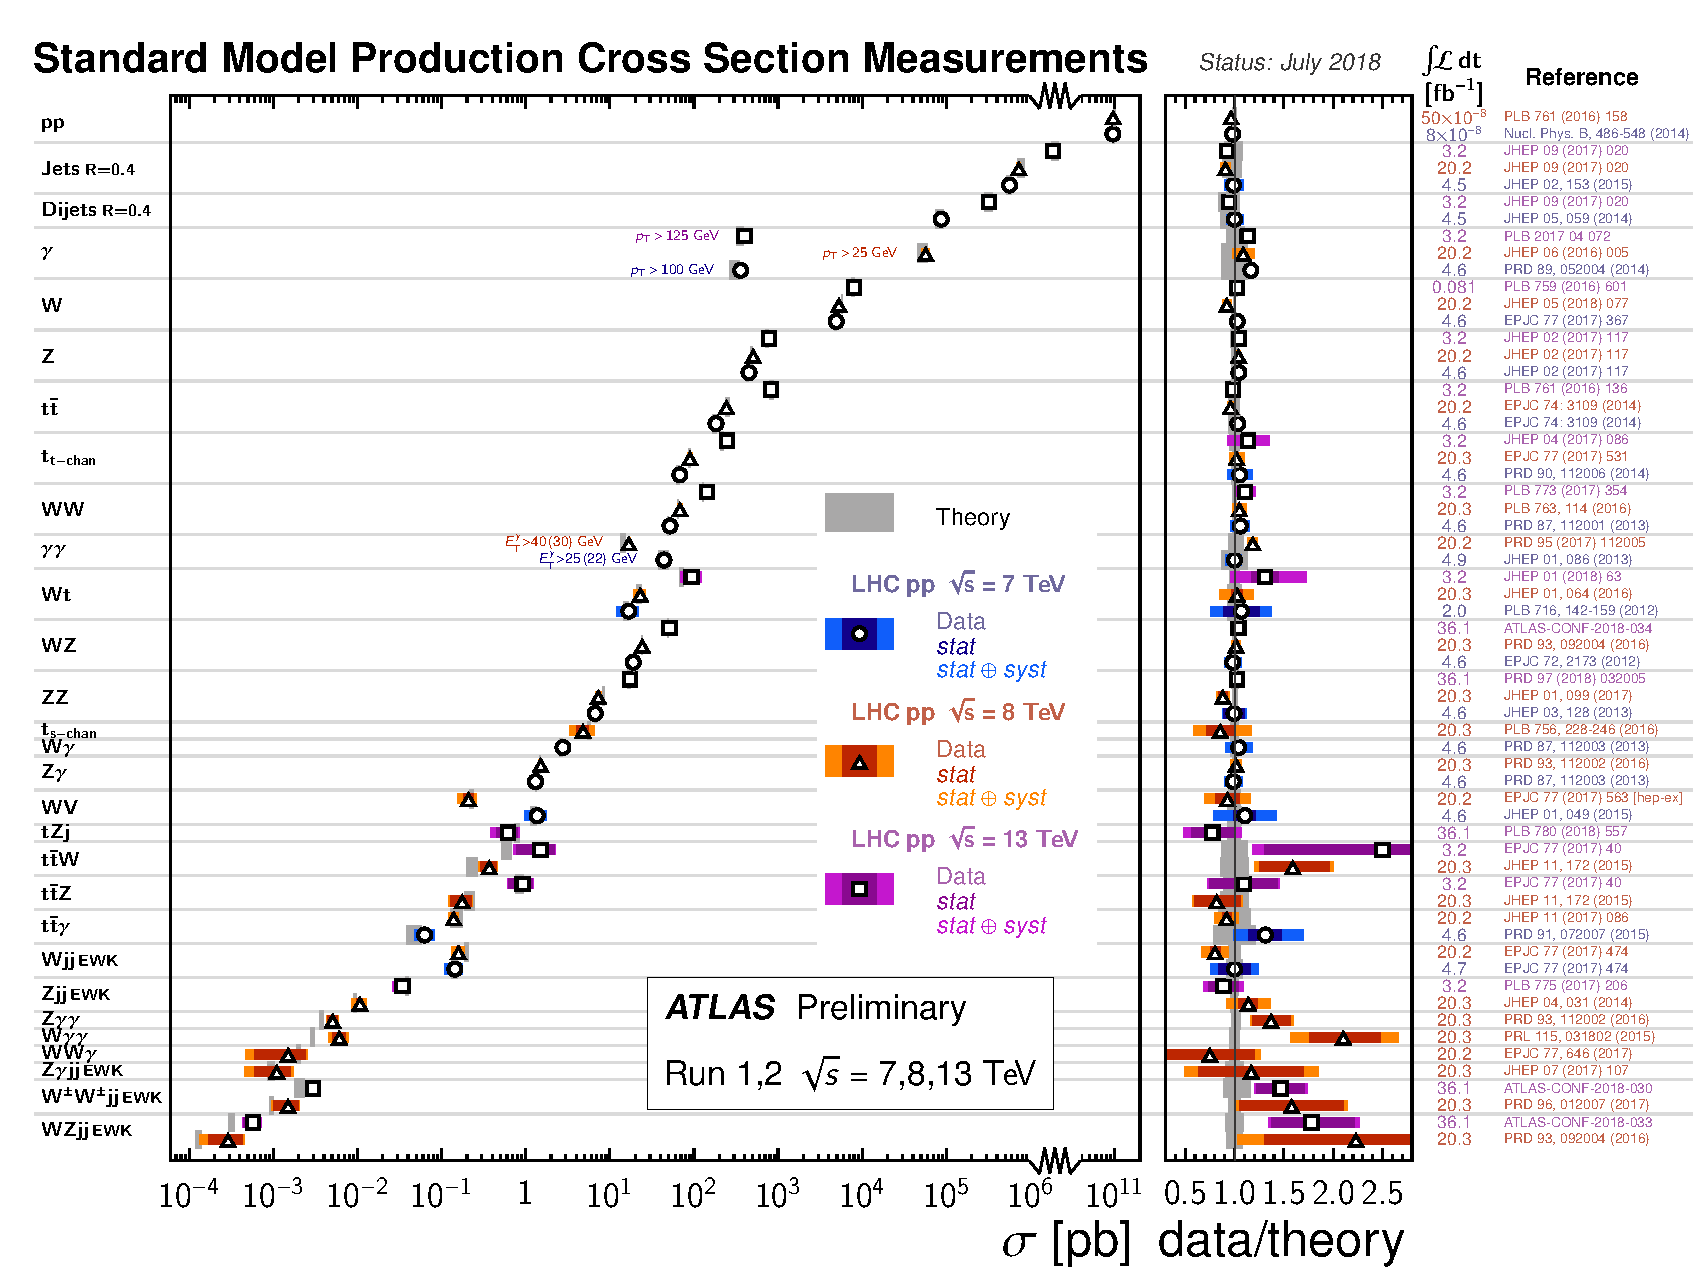
\includegraphics[width=\textwidth]{theory/ATLAS_SMSummary_FiducialXsect_rotated.eps}
 \caption[Summary of several Standard Model total and fiducial production cross section measurements using LHC proton-proton collisions, corrected for leptonic branching fractions, compared to the corresponding theoretical expectations.]{%
  Summary of several Standard Model total and fiducial production cross section measurements using LHC proton-proton collisions, corrected for leptonic branching fractions, compared to the corresponding theoretical expectations.
  All theoretical expectations were calculated at NLO or higher.
  The dark-color uncertainty bar represents the statistical uncertainty.
  The lighter-color uncertainty bar represents the full uncertainty, including systematics and luminosity uncertainties.
  The data/theory ratio, luminosity used and reference for each measurement are also shown.
  Uncertainties for the theoretical predictions are quoted from the original ATLAS papers.
  They were not always evaluated using the same prescriptions for PDFs and scales.
  The $W\gamma$ and $Z\gamma$ theoretical cross-sections have non-perturbative corrections applied to the NNLO fixed order calculations~\cite{STDM-2011-17}.
  Not all measurements are yet statistically significant~\cite{web:ATLAS_SM_summary_plots}.}
 \label{fig:cross_section_experiment_theory}
\end{figure}

The quanta of the quantum fields of the Standard Model are the particles of matter and the mediators of the fundamental forces of Nature, shown in \Cref{fig:Standard_Model}.
The spin-$1/2$ fermion fields result in the three ``generations'' of the six quarks and six leptons, which compose all matter in the Universe.
The leptons are divided into the electrically charged leptons --- the electron $(e)$, muon $(\mu)$, and tau $(\tau)$ --- and their electrically neutral neutrino counterparts --- ``flavor'' eigenstates of $\nu_{e}$, $\nu_{\mu}$, and $\nu_{\tau}$.
The quarks have fractional electric charge, with the up $(u)$, charm $(c)$, and top $(t)$ quarks having $+2/3$ elementary charge, and the down $(d)$, strange $(s)$, and bottom $(b)$ quarks having $-1/3$, as well as all of them carrying a ``color'' charge that allows them to participate in strong nuclear interactions.
They do not exist as free particles by themselves, but always in bound configurations of either two or three quarks, respectively known as ``mesons'' and ``baryons'' (e.g., pions and protons, respectively).
In addition to the matter particles are the five vector gauge bosons that are mediators of fundamental forces of Nature.
The photon $(\gamma)$ is the mediator of the electromagnetic force and interacts with all particles that carry electrical charge (i.e. the quarks, charged leptons, and charged vector bosons).
The weak nuclear force that governs nuclear interactions, such as beta decay, is mediated by the $W^{+}$, $W^{-}$, and $Z$ massive weak vector bosons.
The electrically charged $W$ bosons mediate charged flavor changing interactions between the quarks and the leptons (e.g., $c \to d + W^{+}$ and $e^{-} \to \bar{\nu}_{e} + W^{-}$), and the $Z$ boson mediates electrically neutral flavor changing interactions (e.g., $e^{+}e^{-} \to Z \to \mu^{+}\mu^{-}$ and charged lepton scattering from neutrinos).
The eight%
\footnote{As a result of the $\mathrm{SU}(3)$ symmetry.}
massless gluons mediate the strong nuclear force and so have couplings with all particles that have color charge: the quarks and the gluons themselves.
The coupling strength of the gluons varies with distance between color charged particles --- being extremely strong at close ranges and then sharply dropping of at the distance of confinement (approximately the radius of the proton).
Finally, the Higgs boson imparts mass to particles that it couples to, with stronger coupling strengths manifesting as larger masses.
This process --- which has been come to be known as the ``Higgs mechanism'' --- gives rise to the non-zero mass of the $W^{\pm}$ and $Z$ through a processes called ``electroweak symmetry breaking'' and will be discussed more throughly in \Cref{section:EWSB}.

\begin{figure}
 \centering
 \includegraphics[width=\textwidth]{theory/Standard_Model.pdf}
 \caption[Diagram of the particles of the Standard Model.]{%
  Diagram of the particles of the Standard Model.
  Shown are the three generations of fermions (the quarks and leptons), the gauge vector bosons (gluons, photon, $W^{\pm}$, and $Z$), and the Higgs boson.
  This figure was inspired and adapted from~\cite{web:Carsten_Burgard}.}
 \label{fig:Standard_Model}
\end{figure}

The following discussion of the theories that compose the Standard Model is my summary of many post-lecture conversations with former SMU professor Kent Hornbostel and readings of~\cite{Pich:2005mk}.

\section{Quantum Field Theories}\label{section:QFT}

\acrlong{QFT} is the mathematical framework for modern particle physics calculations.
QFT naturally incorporates quantum theory with special relativity to give a relativistic description of the interaction of quantum fields through their quantized excitations (particles).
All possible physical interactions of these fields are encoded in the terms of the Lagrangian density, $\Lagrangian$, which is a scalar and so (crucially) Lorentz invariant --- physics fundamentally works the same regardless of reference frame.
Given the ubiquity of the use of the Lagrangian density in calculations it will be interchangeably referred to as the ``Lagrangian'' henceforth, with hopefully minimal confusion.
Additionally, the Lagrangian density must be locally gauge invariant; meaning that it is invariant under certain Lie group transformations.
Local gauge invariance is an expression that representations of the Lagrangian density that result in the same physical interactions must be equivalently valid.
A local gauge symmetry is distinct from a global gauge symmetry, as would arise in Noether's theorem, in that a local gauge symmetry results in a gauge invariance for the spacetime point of consideration, but is not guaranteed to be valid in all cases.
That is, a global gauge symmetry is in some sense a special case of a local gauge symmetry, where the symmetry applies for all points.
As an example, consider the Dirac Lagrangian
\begin{equation}
 \Lagrangian_{\textrm{Dirac}} = \bar{\psi} \left(i \gamma^{\mu}\partial_{\mu} - m\right)\psi.
 \label{eq:Dirac_Lagrangian}
\end{equation}
If a global gauge transformation of a phase shift is applied,
\[
 \psi \to e^{-i\theta} \psi, \qquad \bar{\psi} \to \bar{\psi}\,e^{i\theta},
\]
then it is readily seen that the Lagrangian has remained invariant
\[
 \Lagrangian \to \bar{\psi} \left(i \gamma^{\mu}\partial_{\mu} - m\right)\psi.
\]
However, if a local gauge transformation of a phase shift dependent on the field's spacetime is applied
\[
 \psi \to e^{-i\theta(x)} \psi, \qquad \bar{\psi} \to \bar{\psi}\,e^{i\theta(x)},
\]
then for the Lagrangian
\[
 \Lagrangian \to \bar{\psi} \left(i \gamma^{\mu}\partial_{\mu} - m\right)\psi + \bar{\psi}\, \gamma^{\mu} \left(\partial_{\mu} \theta\right)\psi
\]
to preserve the definition of the four-gradient under such a local transformation requires the addition of a gauge field $A_{\mu}(x)$ to form the covariant%
\footnote{``Covariant'' in that it transforms with the gauge fields so that the derivative remains unchanged.}
derivative,
\[
 D_{\mu} \equiv \partial_{\mu} - iq A_{\mu}(x),
\]
with local gauge transformation
\[
 A_{\mu} \to A_{\mu} - \frac{1}{q} \partial_{\mu}\theta,
\]
such that
\[
 \theta(x) = q \Lambda(x),
\]
resulting in the nice covariant form
\[
 \Lagrangian \to \bar{\psi} \left(i \gamma^{\mu}D_{\mu} - m\right)\psi = \bar{\psi} \left(i \slashed{D} - m\right)\psi.
\]
Given the implications of local gauge invariance, the gauge may be arbitrarily chosen to simplify calculations with no less of generality.

Two examples of highly successful \glspl{QFT} are \gls{QED} and \gls{QCD}, which are briefly discussed here.

\subsection{Quantum Electrodynamics (QED)}\label{subsection:QED}

The Glashow-Weinberg-Salam theory of electromagnetic interactions~\cite{Glashow:1961tr,Goldstone:1962es,Weinberg:1967tq} defines electromagnetic interactions of matter in the Standard Model.
The Lagrangian density for QED --- which describes the interactions of a spin-$1/2$ field with the electromagnetic field --- possesses a global $\mathrm{U}(1)$ symmetry, manifest through the conservation of electric charge, and is given by
\begin{equation}
 \Lagrangian_{\textrm{QED}} = -\frac{1}{4}F_{\mu\nu} F^{\mu\nu} + \bar{\psi} \left(i \slashed{D} - m\right)\psi
 \label{eq:QED_Lagrangian}
\end{equation}
where $F_{\mu\nu} = \partial_{\mu}A_{\nu} - \partial_{\nu}A_{\mu}$ is the electromagnetic field strength tensor.
In the QED Lagrangian, the kinetic term $-\frac{1}{4}F_{\mu\nu} F^{\mu\nu}$ describes the behavior of the electromagnetic field --- which along with the Euler-Lagrange equations result in Maxwell's equations --- and the term $\bar{\psi} \left(i \slashed{D} - m\right)\psi$ gives the interactions of the electromagnetic field with charged particles.

\subsection{Quantum Chromodynamics (QCD)}\label{subsection:QCD}

\gls{QCD} is the gauge field theory that describes the interactions of quarks and gluons governed by the strong nuclear force, and characterized by a $\mathrm{SU}(3)$ symmetry.
The QCD Lagrangian density is
\begin{equation}
 \Lagrangian_{\textrm{QCD}} = -\frac{1}{4}G_{\mu \nu}^{a} G_{a}^{\mu \nu} + \sum_{f} i \bar{\psi}_{f} D_{\mu} \gamma^{\mu} \psi_{f},
 \label{eq:QCD_Lagrangian}
\end{equation}
for the $f$ families of quarks, $\psi_{f}$.
The Lagrangian is written without the color index for readability, but, as both the quarks and gluons carry a color charge, then the quark fields $\psi$ are column vectors with color index $\alpha$ and the gluon fields $G_{\mu}^{a}$ are matrices with color indices $\alpha$ and $\beta$.
The kinetic term $-\frac{1}{4}G_{\mu \nu}^{a} G_{a}^{\mu \nu}$ describes the self interactions of the gluon fields $G_{\mu}^{a}$ given the gluon field strength tensor $G_{\mu\nu}^{a} = \partial_{\mu} G_{\nu}^{a} - g_{s} f^{abc} G_{\mu}^{b} G_{\nu}^{c}$
for strong coupling constant $g_{s}$ and $\mathrm{SU}(3)$ structure constants $f^{abc}$.
The term $\sum_{f} i \bar{\psi}_{f} D_{\mu} \gamma^{\mu} \psi_{f}$ with covariant derivative
\[
 D_{\mu} = \partial_{\mu} - i g_{s} G_{\mu}^{a} T^{a},
\]
where $T^{a}$ are the generators of the $\mathrm{SU}(3)$ symmetry group, is the kinetic term for the quarks and describes the interactions between quarks and gluons.
QCD is a deeply rich theory that deserves much attention (c.f.~\cite{Campbell:2017hsr}), but for the purposes of this thesis it will only be introduced here to motivate a more complete picture of the QFTs that build the Standard Model.

\section{Spontaneous Symmetry Breaking}\label{section:symmetry_breaking}

Spontaneous symmetry breaking is the process by which a physical system that has a symmetry does not express that symmetry for perturbations around the ground state of the system.
It is worth noting, given the somewhat confusing nature of the use of ``breaking,'' that the symmetry of the Lagrangian is not destroyed under symmetry breaking, but rather is not manifest given the ground state into which the system has been perturbed.
A classical example of spontaneous symmetry breaking is that of a pen being balanced upright on its tip on a table.
In the unstable equilibrium state of the pen being balanced (the high energy/excited state configuration) the pen possesses a $\mathrm{U}(1)$ symmetry of rotation about its axis.
If the pen is perturbed from this state by a small vibration it will fall into its ground state onto the surface of the table and will lie along some direction ``breaking'' the symmetry that was exhibited by the previous state.
Another example is that of Heisenberg’s model of the ferromagnet, which has Hamiltonian of $\mathcal{H} = -\sum_{i\neq j} J_{ij}\,\vec{s}_{i} \cdot \vec{s}_{j}$ across neighboring atoms.
This Hamiltonian also possesses as rotational symmetry above the Curie temperature --- rotating all the spins by some amount leaves the total spin of the system invariant.
However, below the Curie temperature a non-zero magnetization will arise along a particular direction which will cause all spins to become aligned parallel to it, breaking the symmetry.

A final illustrative toy model, that will prove useful in the context of the Higgs mechanism, is that of a massive complex scalar field
\[
 \phi = \frac{1}{\sqrt{2}} \left(\phi_{1} + i \phi_{2}\right),
\]
with Lagrangian density
\[
 \Lagrangian = \partial_{\mu}\phi^{\dagger}\partial^{\mu}\phi - m^{2}\phi^{\dagger}\phi + \frac{\lambda}{4} \left(\phi^{\dagger}\phi\right)^{2}
\]
composed of the kinetic term, $\partial_{\mu}\phi^{\dagger}\partial^{\mu}\phi$, and the potential $V\left(\phi\right) = -m^{2}\phi^{\dagger}\phi + \frac{\lambda}{4} \left(\phi^{\dagger}\phi\right)^{2}$.
The potential is zero at $\phi=0$, but has its minima occur at
\[
 \phi^{\dagger}\phi = \frac{1}{2}\left(\phi_{1}^{2} - \phi_{2}^{2}\right) = \frac{2m^2}{\lambda} \equiv \frac{1}{2}v^{2}
\]
with magnitude
\[
 \abs{\phi} = \frac{1}{\sqrt{2}}v = \frac{\sqrt{2} v}{\lambda^{1/2}}.
\]
It is seen that this potential possesses a $\mathrm{U}(1)$ symmetry, such that it is invariant under $\phi \to e^{-i\theta}\phi$, resulting in an infinite number of possible minima.
Rewriting the fields using polar coordinates in field space,
\[
 \phi(x) = \frac{1}{\sqrt{2}} \rho\left(x\right) e^{-i \theta(x)/v},
\]
and choosing the arbitrary ground state --- breaking the symmetry --- of $\rho=v$ and $\theta=0$ then allows for the redefinition of the fields as
\[
 \phi(x) = \frac{1}{\sqrt{2}} \left(v + h\left(x\right)\right) e^{-i \theta(x)/v},
\]
where $h$ and $\theta$ become the normal modes.
Perturbations about the minima result in massive radial $h$ modes and massless rotational $\theta$ modes.
These radial modes result in a massive particle, and the rotational modes result in massless particles known as Nambu-Goldstone bosons~\cite{Nambu:1960tm,Goldstone:1961eq}.

\section{Electroweak Symmetry and Interactions}\label{section:EW_interactions}

The electroweak interactions are encoded in the symmetry group $\mathrm{SU}(2)_{L} \otimes \mathrm{U}(1)_{Y}$, where $\mathrm{SU}(2)$ is the symmetry of weak-isospin and $Y$ is weak-hypercharge.
The gauge group requires all left-handed spinors to be doublets, and the right-handed spinors to be singlets.
Considering only the first generation of quarks and leptons, this can be written for the leptons as
\[
 \psi_{e\,1}\left(x\right) = \begin{pmatrix}
  \nu_{e} \\
  e^{-}
 \end{pmatrix}_{L},\quad
 \psi_{e\,2}\left(x\right) = \nu_{e\,R},\quad
 \psi_{e\,3}\left(x\right) = e_{R}^{-}\,,
\]
and for the quarks as
\[
 \psi_{u\,1}\left(x\right) = \begin{pmatrix}
  u \\
  d
 \end{pmatrix}_{L},\quad
 \psi_{u\,2}\left(x\right) = u_{R},\quad
 \psi_{u\,3}\left(x\right) = d_{R}\,.
\]
The ``free'' Lagrangian density (the kinetic term) is then
\[
 \Lagrangian = \sum_{j=1}^{3} i \,\bar{\psi}_{e\,j}\left(x\right) \slashed{\partial} \,\psi_{e\,j}\left(x\right) + i \,\bar{\psi}_{u\,j}\left(x\right) \slashed{\partial} \,\psi_{u\,j}\left(x\right)\,,
\]
which should be invariant under local gauge transformations of the symmetry group,
\[
 \begin{split}
  \psi_{e\,1}&\left(x\right) \to e^{iy_{1} \beta(x)}\, U_{L}\left(x\right)\psi_{e\,1}\left(x\right), \qquad U_{L}\left(x\right) = \exp\left(i\,\frac{\tau^{i}}{2} \alpha^{i}(x)\right)\\
  \psi_{e\,2}&\left(x\right) \to e^{iy_{2} \beta(x)}\, \psi_{e\,2}\left(x\right)\\
  \psi_{e\,3}&\left(x\right) \to e^{iy_{3} \beta(x)}\, \psi_{e\,3}\left(x\right)
 \end{split}
\]
The generators of $\mathrm{SU}(2)$ are the Pauli spin matrices,
\[
 \tau^{0} = \begin{pmatrix}%
  1 & 0 \\%
  0 & 1
 \end{pmatrix},\quad
 \tau^{1} = \begin{pmatrix}%
  0 & 1 \\%
  1 & 0
 \end{pmatrix},\quad
 \tau^{2} = \begin{pmatrix}%
  0 & -i \\%
  i & 0
 \end{pmatrix},\quad
 \tau^{3} = \begin{pmatrix}%
  1 & 0  \\%
  0 & -1 %
 \end{pmatrix}\,,%
\]
and the resulting four degrees of freedom (three from $\mathrm{SU}(2)$ and one from $\mathrm{U}(1)$) manifest as the gauge bosons of the weak vector fields $W_{\mu}^{k}\left(x\right)$:
\[
 B_{\mu}\left(x\right) = W_{\mu}^{0}\left(x\right)\tau^{0}, \qquad \vec{W}_{\mu}\left(x\right) = W_{\mu}^{i}\left(x\right)\frac{\tau^{i}}{2}\,.
\]
As a result, the covariant derivative is
\begin{align}
 D_{\mu}\psi_{1}(x) & = \left(\partial_{\mu} - ig_{1}\, y_{1} B_{\mu}(x) - ig_{2} \vec{W}_{\mu}(x)\right)\psi_{1}(x)\label{eq:EW_derivative} \\
 D_{\mu}\psi_{2}(x) & = \left(\partial_{\mu} - ig_{1}\, y_{2} B_{\mu}(x)\right)\psi_{2}(x)\notag                                             \\
 D_{\mu}\psi_{3}(x) & = \left(\partial_{\mu} - ig_{1}\, y_{3} B_{\mu}(x)\right)\psi_{3}(x)\notag
\end{align}
for weak hypercharge $y_{i}$ coupling $g_{1}$ and weak isospin coupling $g_{2}$, this gives the requirements for the local transformations of the vector gauge fields,
\[
 B_{\mu}(x) \to B_{\mu}(x) + \frac{1}{g_{1}} \partial_{\mu}\beta(x), \qquad%
 \vec{W}_{\mu}(x) \to U_{L}(x)\vec{W}_{\mu}(x)\,U_{L}^{\dagger}(x) - \frac{i}{g_{2}} \left(\partial_{\mu}U_{L}(x)\right)
 U_{L}^{\dagger}(x)
\]
The kinetic term of the electroweak vector gauge field Lagrangian density is then seen to be
\[
 \Lagrangian_{\textrm{kinetic}} = -\frac{1}{4}B_{\mu\nu}B^{\mu\nu} - \frac{1}{2}\mathrm{Tr}\left(\vec{W}_{\mu\nu}\vec{W}^{\mu\nu}\right) = -\frac{1}{4}B_{\mu\nu}B^{\mu\nu} -\frac{1}{4} W_{\mu\nu}^{i} W_{i}^{\mu\nu}.
\]
It is seen that the $\mathrm{SU}(2)_{L} \otimes \mathrm{U}(1)_{Y}$ gauge symmetry forbids a mass term for the vector fields, and fermion masses are also forbidden as the term would mix the left and right handed fields which have different transformation properties --- which would explicitly break the gauge symmetry.

\subsection{Electroweak Interactions}

Given the covariant derivative, \Cref{eq:EW_derivative}, and resulting Lagrangian density for the fermions,
\[
 \Lagrangian = \sum_{j=1}^{3} i \,\bar{\psi}_{e\,j}\left(x\right) \slashed{D} \,\psi_{e\,j}\left(x\right) + i \,\bar{\psi}_{u\,j}\left(x\right) \slashed{D} \,\psi_{u\,j}\left(x\right)\,,
\]
it is seen that there are interactions between the fermions and the vector gauge fields (dropping fermion index for compactness),
\[
 \Lagrangian \subset g_{2} \bar{\psi}_{1} \gamma^{\mu}\vec{W}_{\mu} \psi_{1} + g_{1} B_{\mu} \sum_{j=1}^{3} y_{j}\bar{\psi}_{j} \gamma^{\mu} \,\psi_{j}\,.
\]
The first term, which contains the $\mathrm{SU}(2)_{L}$ matrix
\[
 \vec{W}_{\mu} = W_{\mu}^{i}(x) \frac{\tau^{i}}{2} = \frac{1}{\sqrt{2}} \begin{pmatrix}%
  \sqrt{2} W_{\mu}^{3} & W_{\mu}^{\dagger}     \\
  W_{\mu}              & -\sqrt{2} W_{\mu}^{3}
 \end{pmatrix}\,,
\]
gives rise to the charged current interactions of the charged $W$ boson fields
\[
 W_{\mu} = \frac{1}{\sqrt{2}} \left(W_{\mu}^{1}  + i W_{\mu}^{2}\right), \qquad W_{\mu}^{\dagger} = \frac{1}{\sqrt{2}} \left(W_{\mu}^{1}  - i W_{\mu}^{2}\right)
\]
with the left-handed quarks and charged leptons, seen in \Cref{fig:EW_W_quarks} and \Cref{fig:EW_W_leptons}.
Likewise, through mixing of the neutral $W_{\mu}^{3}$ and $B_{\mu}$ fields,
\[
 \begin{pmatrix}
  A_{\mu} \\
  Z_{\mu}
 \end{pmatrix}
 = \begin{pmatrix}
  \cos\theta_{W}  & \sin\theta_{W} \\
  -\sin\theta_{W} & \cos\theta_{W}
 \end{pmatrix}
 \begin{pmatrix}
  B_{\mu} \\
  W_{\mu}^{3}
 \end{pmatrix}\,,
\]
with Weinberg mixing angle
\[
 \sin\theta_{W} = \frac{g_{1}}{\sqrt{g_{1}^{2} + g_{2}^{2}}}, \qquad \cos\theta_{W} = \frac{g_{2}}{\sqrt{g_{1}^{2} + g_{2}^{2}}},
\]
the mass eigenstates of the $Z$ boson and photon arise
\[
 \begin{split}
  Z_{\mu} &= W_{\mu}^{3} \cos\theta_{W} - B_{\mu} \sin\theta_{W} = \frac{1}{\sqrt{g_{1}^{2} + g_{2}^{2}}} \left(g_{2} W_{\mu}^{3} - g_{1} B_{\mu}\right) \\
  A_{\mu} &= W_{\mu}^3 \sin\theta_{W} + B_{\mu} \cos\theta_{W} = \frac{1}{\sqrt{g_{1}^{2} + g_{2}^{2}}} \left(g_{1} W_{\mu}^{3} + g_{2} B_{\mu}\right)
 \end{split}
\]
which mediate the neutral current interactions with the fermions, seen in \Cref{fig:EW_Z} and \Cref{fig:QED_photon}.

\begin{figure}[htbp]
 \centering
 \begin{subfigure}[t]{0.23\textwidth}
  \centering
  \includegraphics[width=\textwidth]{theory/QED_photon.pdf}
  \caption[The vertex for interactions of an electrically charged particle and a photon.]{%
   The vertex for interactions of an electrically charged particle and a photon.}
  \label{fig:QED_photon}
 \end{subfigure}%
 \quad
 \begin{subfigure}[t]{0.23\textwidth}
  \centering
  \includegraphics[width=\textwidth]{theory/electroweak_Z.pdf}
  \caption[The vertex for neutral current interactions of an fermion and a $Z$ boson.]{%
   The vertex for neutral current interactions of an fermion and a $Z$ boson.}
  \label{fig:EW_Z}
 \end{subfigure}%
 \quad
 \begin{subfigure}[t]{0.23\textwidth}
  \centering
  \includegraphics[width=\textwidth]{theory/electroweak_W_quarks.pdf}
  \caption[The vertex for charged current interactions of quarks with a $W$ boson.]{%
   The vertex for charged current interactions of quarks with a $W$ boson.}
  \label{fig:EW_W_quarks}
 \end{subfigure}%
 \quad
 \begin{subfigure}[t]{0.23\textwidth}
  \centering
  \includegraphics[width=\textwidth]{theory/electroweak_W_leptons.pdf}
  \caption[The vertex for charged current interactions of a charged lepton and neutrino with a $W$ boson.]{%
   The vertex for charged current interactions of a charged lepton and neutrino with a $W$ boson.}
  \label{fig:EW_W_leptons}
 \end{subfigure}%
 \caption[The Feynman diagrams for allowed QED and electroweak interactions.]{%
  The Feynman diagrams for allowed QED and electroweak interactions in the Standard Model.}
 \label{fig:electroweak_vertices}
\end{figure}

\section{Electroweak Symmetry Breaking}\label{section:EWSB}

To break the electroweak symmetry and provide masses to the weak vector bosons, consider the discussion given in \Cref{section:symmetry_breaking} and a complex scalar doublet (introduced by, among others~\cite{Guralnik:1964eu,Kibble:2015mwa}, Brout and Englert~\cite{Englert:1964et}, and Higgs~\cite{Higgs:1964ia,Higgs:1964pj})
\begin{equation}
 \phi = \begin{pmatrix}%
  \phi^{+} \\%
  \phi^{0}
 \end{pmatrix} = \frac{1}{\sqrt{2}} \begin{pmatrix}%
  \phi_{1} + i \phi_{2} \\%
  \phi_{3} + i \phi_{4}%
 \end{pmatrix}%
 \label{eq:Higgs_doublet}
\end{equation}
with Lagrangian density
\begin{equation}
 \Lagrangian_{\textrm{Higgs}} = \left(D_{\mu}\phi\right)^{\dagger}D^{\mu}\phi - \mu^{2}\phi^{\dagger}\phi + \lambda \left(\phi^{\dagger}\phi\right)^{2}
 \label{eq:Higgs_Lagrangian}
\end{equation}
that is invariant under local $\mathrm{SU}(2)_{L} \otimes \mathrm{U}(1)_{Y}$ transformations.
The Higgs potential
\begin{equation}
 V\left(\phi\right) = -\mu^{2}\phi^{\dagger}\phi + \lambda \left(\phi^{\dagger}\phi\right)^{2},
 \label{eq:Higgs_potential}
\end{equation}
shown in \Cref{fig:Higgs_potential}, is chosen such that $\mu^{2} < 0$ and $\lambda > 0$ to provide stable minima.
As before in \Cref{section:symmetry_breaking} with the case of the toy model of the massive complex scalar field, once a ground state has been arbitrarily chosen this spontaneously breaks the $\mathrm{SU}(2)_{L} \otimes \mathrm{U}(1)_{Y}$ symmetry to the subgroup $\mathrm{U}(1)_{\textrm{QED}}$.
This time, the four fields of the complex scalar doublet are reparameterized into
\[
 \phi(x) = \frac{1}{\sqrt{2}} \begin{pmatrix}
  0 \\
  v + h(x)
 \end{pmatrix}
 \exp\left(i \frac{\tau^{i}}{2} \theta^{i}(x)\right)
\]
which gives the real scalar field $h(x)$, corresponding to radial perturbations of the minima, and three%
\footnote{There is much beauty in electroweak symmetry breaking, but the simple, insightful choice of the doublet to give as many Nambu-Goldstone bosons as vector gauge fields is marvelous.}
Nambu-Goldstone fields $\theta^{i}(x)$ with rotational symmetry --- their values have become gauge choices.
Exploiting this gauge freedom, and choosing the unitary gauge $\theta^{i}(x)=0$, results in kinetic term $\left(\textrm{where } g = \sqrt{g_{1}^{2} + g_{2}^{2}}\right)$
\[
 \Lagrangian \subset \frac{1}{2}\partial_{\mu} h \partial^{\mu} h + \left(v + h\right)^{2} \left(\frac{g^{2}}{4} W_{\mu}^{\dagger}W^{\mu} + \frac{g^{2}}{8 \cos^2 \theta_{W}} Z_{\mu}^{\dagger}Z^{\mu}\right)
\]
where the $W^{\pm}$ and $Z$ bosons have absorbed the Nambu-Goldstone bosons as polarizations and respectively acquired masses of
\[
 m_{W} = \frac{1}{2}vg, \qquad m_{Z} = \frac{m_{W}}{\cos\theta_{W}} = \frac{vg}{2\cos\theta_{W}}\,.
\]
The scalar field --- the Higgs field --- also acquires a mass term of
\[
 m_{h} = \sqrt{-2\mu^{2}} = \sqrt{2h}v.
\]
In the Standard Model $v$, $g_{1}$, $g_{2}$ are free parameters to be measured by experiment, and so the masses of the bosons are not directly predicted.
However, the value%
\footnote{Often referred to as the ``weak scale'' or the ``vacuum expectation value.''}
of $v$ has been calculated independently~\cite{Plehn:2005nk} to be approximately $246~\GeV$.
It is also noted that in further interactions the quarks and charged leptons acquire a mass term from Yukawa couplings~\cite{Yukawa:1935xg}, $c_i$, with the Higgs field
\[
 \begin{split}
  \Lagrangian_{\textrm{Yukawa}} &= -\frac{1}{\sqrt{2}} \left(v+h\right) \left(c_{1}\bar{d}d + c_{2}\bar{u}u + c_{3}\bar{e}e\right) \\
  &= - \left(1 + \frac{h}{v}\right)\left(m_{d}\bar{d}d + m_{u}\bar{u}u + m_{e}\bar{e}e\right)\,.
 \end{split}
\]
The neutrinos notably do not participate in this interaction, and their observed non-zero mass~\cite{Ahmad:2001an} is unexplained through electroweak symmetry breaking in the Standard Model and is currently unresolved.

\begin{figure}[htbp]
 \centering
 \includegraphics[width=\linewidth]{theory/higgs_potential.pdf}
 \caption[Sketch of the Higgs potential shape.]{%
 Sketch of the Higgs potential's ``winebottle'' shape.
 The trough (the bottom of the eponymous winebottle) are the infinite choices of minima at the vacuum expectation value, $v$, that can be chosen from upon spontaneously breaking the $\mathrm{SU}(2)_{L} \otimes \mathrm{U}(1)_{Y}$ symmetry to the subgroup $\mathrm{U}(1)_{\textrm{QED}}$.}
 \label{fig:Higgs_potential}
\end{figure}

\section{The Higgs Boson}\label{section:Higgs_boson}

The massive Higgs boson produced though the ``Higgs mechanism'' approach to electroweak symmetry breaking is a particle of great interest, as the interactions of the Higgs field with all other elementary particle fields generates their mass.
As a result, through these couplings the Higgs boson can be produced through a large number of interactions.
As this thesis is focused on experimental efforts at CERN's \gls{LHC}, the production mechanisms of interest will be the leading ones in a hadron collider with center-of-mass energy $\sqrt{s}=13~\TeV$.
In decreasing cross section, those production modes are: gluon-gluon fusion (ggF), vector boson fusion (VBF), vector boson-associated production or ``Higgsstrahlung'' (VH), and associated production with $t\bar{t}$ ($t\bar{t}H$), seen in \Cref{fig:Higgs_production_diagrams}.
The predicted cross section for these production modes are given in \Cref{table:Higgs_production_cross_section} and plotted with theory uncertainties in \Cref{fig:Higgs_production_cross_section_theory}.

\begin{figure}[htbp]
 \centering
 \begin{subfigure}[t]{0.48\textwidth}
  \centering
  \includegraphics[width=\textwidth]{theory/Higgs_ggF.pdf}
  \caption[Feynman diagram for Higgs production through gluon-gluon fusion.]{%
   Feynman diagram for Higgs production through gluon-gluon fusion.}
  \label{fig:Higgs_ggF}
 \end{subfigure}%
 \quad
 \begin{subfigure}[t]{0.48\textwidth}
  \centering
  \includegraphics[width=\textwidth]{theory/Higgs_VBF.pdf}
  \caption[Feynman diagram for Higgs production through vector boson fusion.]{%
   Feynman diagram for Higgs production through vector boson fusion.}
  \label{fig:Higgs_VBF}
 \end{subfigure}%

 \begin{subfigure}[t]{0.48\textwidth}
  \centering
  \includegraphics[width=\textwidth]{theory/Higgs_strahlung.pdf}
  \caption[Feynman diagram for Higgs production through vector boson associated production (Higgsstrahlung).]{%
   Feynman diagram for Higgs production through vector boson associated production (Higgsstrahlung).}
  \label{fig:Higgs_associated_production}
 \end{subfigure}%
 \quad
 \begin{subfigure}[t]{0.48\textwidth}
  \centering
  \includegraphics[width=\textwidth]{theory/Higgs_ttbar_associated.pdf}
  \caption[Feynman diagram for Higgs production through associated production with $t\bar{t}$.]{%
   Feynman diagram for Higgs production through associated production with $t\bar{t}$.}
  \label{fig:Higgs_associated_production_ttbar}
 \end{subfigure}%
 \caption[The leading production modes at the LHC for Higgs bosons.]{%
  The leading production modes at the LHC for Higgs bosons.}
 \label{fig:Higgs_production_diagrams}
\end{figure}

\begin{table}[htpb]
 \centering
 \caption[The Standard Model Higgs boson production cross sections in units of pb for $m_{H}=125~\GeV$ in $pp$ collisions as a function of the center-of-mass energy, $\sqrt{s}$, at the LHC.]{%
  The SM Higgs boson production cross sections in units of pb for $m_{H}=125~\GeV$ in $pp$ collisions as a function of the center-of-mass energy, $\sqrt{s}$, at the LHC.
  The predictions for the ggF channel include the latest N3LO results leading to reduced theoretical uncertainties by a factor around 2 compared to the N2LO results~\cite{PDG2018:Ch11}.}
 \begin{tabular}{@{}rrrrrrr@{}} \toprule
  $\sqrt{s}~(\TeV)$ & ggF                  & VBF                  & $WH$                 & $ZH$                 & $t\bar{t}H$           & Total~(pb) \\ \midrule
  $13$              & $48.6_{-5\%}^{+5\%}$ & $3.78_{-2\%}^{+2\%}$ & $1.37_{-2\%}^{+2\%}$ & $0.88_{-5\%}^{+5\%}$ & $0.50_{-13\%}^{+9\%}$ & $55.1$     \\
  \addlinespace[0.3em]
  $14$              & $54.7_{-5\%}^{+5\%}$ & $4.28_{-2\%}^{+2\%}$ & $1.51_{-2\%}^{+2\%}$ & $0.99_{-5\%}^{+5\%}$ & $0.60_{-13\%}^{+9\%}$ & $62.1$     \\
  \bottomrule
 \end{tabular}\label{table:Higgs_production_cross_section}%
\end{table}

\begin{figure}
 \centering
 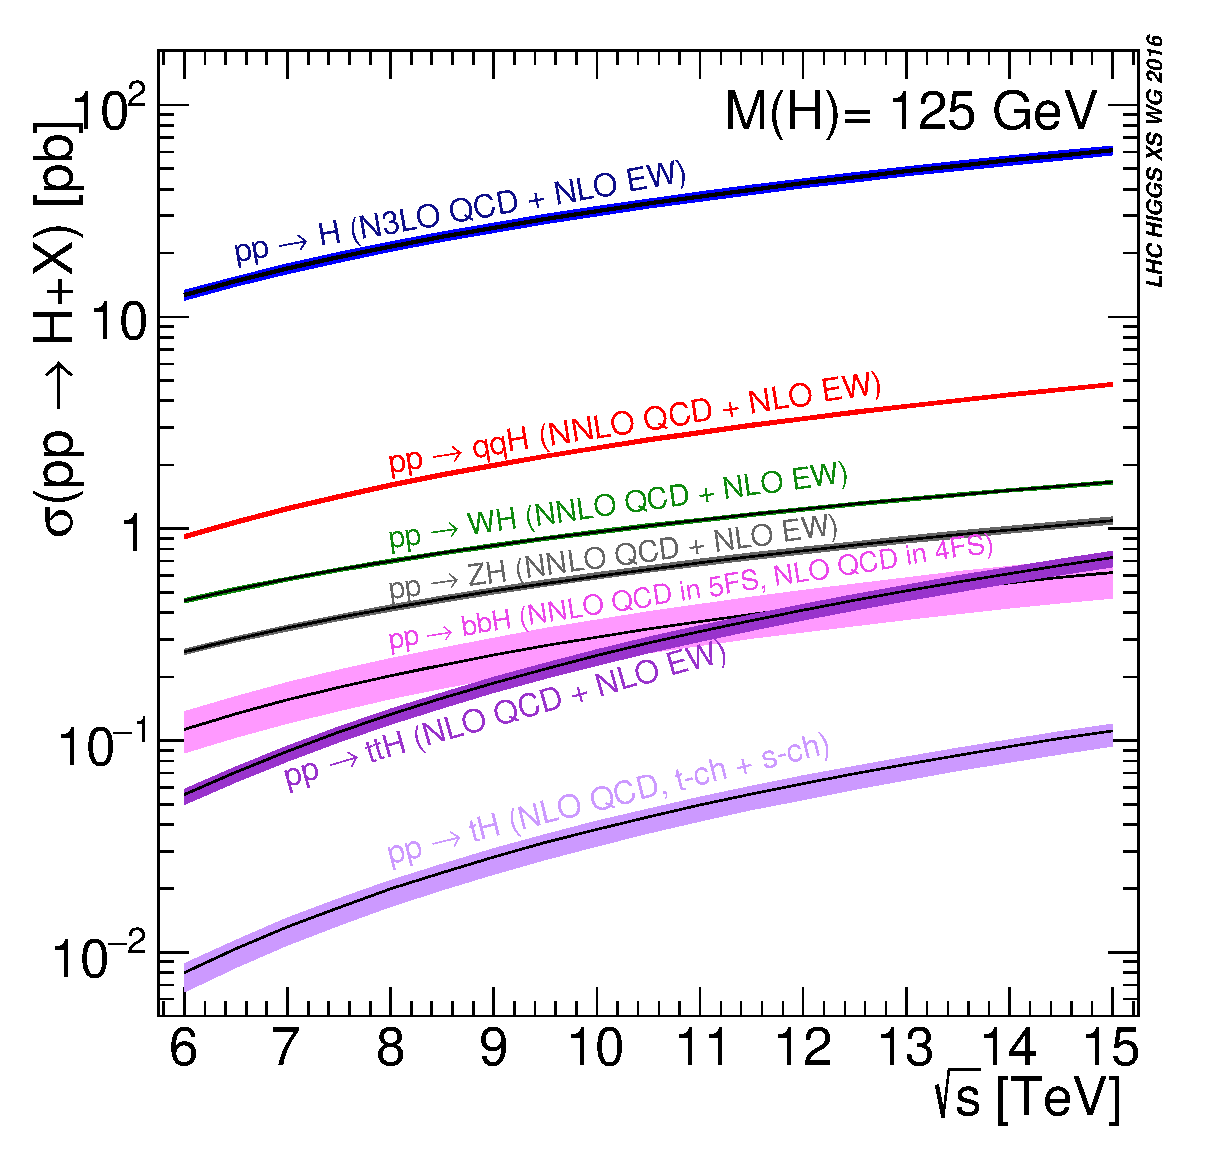
\includegraphics[width=0.5\textwidth]{theory/Higgs_XS_7-14TeV-2016.eps}
 \caption[The Standard Model Higgs boson production cross sections as a function of the center-of-mass energy, $\sqrt{s}$, for $pp$ collisions.]{%
  The Standard Model Higgs boson production cross sections as a function of the center-of-mass energy, $\sqrt{s}$, for $pp$ collisions.
  The VBF process is indicated as $qqH$.
  The theoretical uncertainties are indicated as bands~\cite{PDG2018:Ch11}.}
 \label{fig:Higgs_production_cross_section_theory}
\end{figure}

The SM Higgs has couplings to all the massive vector gauge fields and charged fermions, and so can decay into all of their particles.
At leading order the Higgs will decay primarily to a pair of $b$-quarks $(b\bar{b})$, a pair of weak vector bosons with one of them being off-shell $(VV^{*})$, a pair of gluons $(gg)$, a pair of tau leptons $(\tau^{+}\tau^{-})$, or a pair of photons $(\gamma\gamma)$.
The decays to massless gauge bosons (gluons and photons) are facilitated through loops of massive particles.
The Feynman diagrams for these decays are shown in \Cref{fig:Higgs_decay_channels}, listed in descending (observed) branching ratio in \Cref{table:Higgs_BRs}, and plotted with theory uncertainties in \Cref{fig:Higgs_BRs}.
As the Higgs Yukawa couplings are proportional to the mass of the decay products, it is seen that the Higgs primarily decays to $b\bar{b}$ as $m_{H} < 2 m_{t}$.
However, as hadron colliders mostly produce multijet events%
\footnote{Discovery machines are a messy business.}
from QCD processes, identifying jets coming from resonant $H \to b\bar{b}$ events is quite challenging.

\begin{figure}[htbp]
 \centering
 \begin{subfigure}[t]{0.48\textwidth}
  \centering
  \includegraphics[width=\textwidth]{theory/Hbb.pdf}
  \caption[Feynman diagram for Higgs decay to $b\bar{b}$.]{%
   Feynman diagram for Higgs decay to $b\bar{b}$.}
  \label{fig:H_to_bb}
 \end{subfigure}
 \quad
 \begin{subfigure}[t]{0.48\textwidth}
  \centering
  \includegraphics[width=\textwidth]{theory/H_WW.pdf}
  \caption[Feynman diagram for Higgs decay to $WW^{*}$.]{%
   Feynman diagram for Higgs decay to $WW^{*}$.}
  \label{fig:H_to_WW}
 \end{subfigure}

 \begin{subfigure}[t]{0.48\textwidth}
  \centering
  \includegraphics[width=\textwidth]{theory/Hgg.pdf}
  \caption[Feynman diagram for Higgs decay to $gg$.]{%
   Feynman diagram for Higgs decay to $gg$.}
  \label{fig:H_to_gg}
 \end{subfigure}
 \quad
 \begin{subfigure}[t]{0.48\textwidth}
  \centering
  \includegraphics[width=\textwidth]{theory/Htautau.pdf}
  \caption[Feynman diagram for Higgs decay to $\tau^{+}\tau^{-}$.]{%
   Feynman diagram for Higgs decay to $\tau^{+}\tau^{-}$.}
  \label{fig:H_to_tautau}
 \end{subfigure}

 \begin{subfigure}[t]{0.48\textwidth}
  \centering
  \includegraphics[width=\textwidth]{theory/H_ZZ.pdf}
  \caption[Feynman diagram for Higgs decay to $ZZ^{*}$.]{%
   Feynman diagram for Higgs decay to $ZZ^{*}$.}
  \label{fig:H_to_ZZ}
 \end{subfigure}
 \quad
 \begin{subfigure}[t]{0.48\textwidth}
  \centering
  \includegraphics[width=\textwidth]{theory/H_photons.pdf}
  \caption[Feynman diagram for Higgs decay to $\gamma\gamma$.]{%
   Feynman diagram for Higgs decay to $\gamma\gamma$.}
  \label{fig:H_to_photons}
 \end{subfigure}
 \caption[The leading decay channels of the Higgs boson.]{%
  The leading decay channels of the Higgs boson.}
 \label{fig:Higgs_decay_channels}
\end{figure}

\begin{table}[htpb]
 \centering
 \caption[The branching ratios and the relative uncertainty for a Standard Model Higgs boson with $m_{H}=125~\GeV$.]^{+3.2\%}$ \\
  \addlinespace[0.3em]
  $H\to W^{+}W^{-}$       & $2.14 \times 10^{-1}$ & $_{-4.2\%}^{+4.3\%}$ \\
  \addlinespace[0.3em]
  $H\to \tau^{+}\tau^{-}$ & $6.27 \times 10^{-2}$ & $_{-5.7\%}^{+5.7\%}$ \\
  \addlinespace[0.3em]
  $H\to ZZ$               & $2.62 \times 10^{-2}$ & $_{-4.1\%}^{+4.3\%}$ \\
  \addlinespace[0.3em]
  $H\to \gamma\gamma$     & $2.27 \times 10^{-3}$ & $_{-4.9\%}^{+5.0\%}$ \\
  \addlinespace[0.3em]
  $H\to Z\gamma$          & $1.53 \times 10^{-3}$ & $_{-8.9\%}^{+9.0\%}$ \\
  \addlinespace[0.3em]
  $H\to \mu^{+}\mu^{-}$   & $2.18 \times 10^{-4}$ & $_{-5.9\%}^{+6.0\%}$ \\
  \bottomrule
 \end{tabular}\label{table:Higgs_BRs}%
\end{table}

\begin{figure}
 \centering
 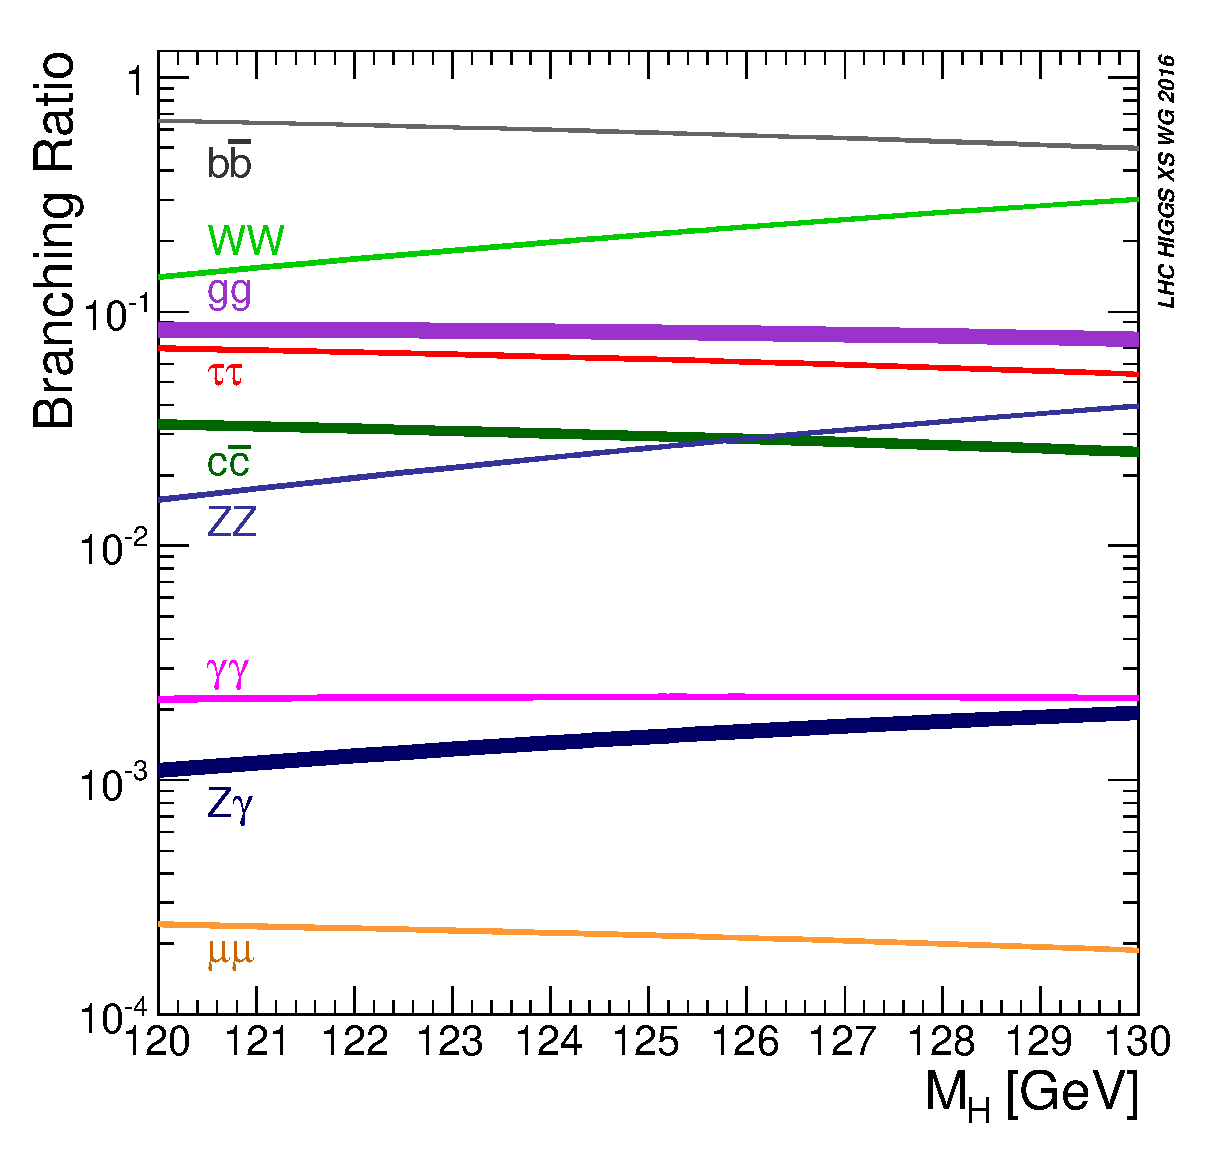
\includegraphics[width=0.5\textwidth]{theory/SMHiggsBR.eps}
 \caption[The branching ratios for the main decays of the Standard Model Higgs boson near $m_{H}=125~\GeV$.]{%
  The branching ratios for the main decays of the Standard Model Higgs boson near $m_{H}=125~\GeV$.
  The theoretical uncertainties are indicated as bands~\cite{PDG2018:Ch11}.}
 \label{fig:Higgs_BRs}
\end{figure}

\section{Extensions to the Standard Model}

To incorporate a model of particle dark matter there are a number of existing extensions of the Standard Model.
Among these are frameworks of simplified dark matter models~\cite{EXOT-2017-32,Jacques:2016dqz,Kahlhoefer:2015bea,Alves:2015pea} where new particles mediate the interactions of dark matter, $\chi$, with the Standard Model particles.
Among these are models for a single neutral vector mediator particle: a $\Zprime$.
One simple extension of the standard model is a vector or axial-vector simplified model through an additional $\mathrm{U}(1)$ gauge symmetry which gives dark matter particles a charge of this symmetry group~\cite{Abercrombie:2015wmb}, and results in either a vector $\left(Z'_{V}\right)$ or axial-vector $\left(Z'_{A}\right)$ boson mediator.
This model introduces five new parameters: the mass of the mediator, $m_{\Zprime}$, the mass of the Dirac fermion dark matter particle, $m_{\chi}$, the flavor-universal coupling of the $\Zprime$ to SM quarks, $g_{q}$, the coupling of the $\Zprime$ to all lepton flavors, $g_{\ell}$, and the coupling of the $\Zprime$ to dark matter, $g_{\chi}$.
The resulting interactions of the $\Zprime$ mediator and the particles are shown in \Cref{fig:Zprime_interactions}.

\begin{figure}[htbp]
 \centering
 \begin{subfigure}[t]{0.48\textwidth}
  \centering
  \includegraphics[width=\textwidth]{theory/Zprime_SM_coupling.pdf}
  \caption[Feynman diagram of the interactions of the $\Zprime$ mediator with Standard Model fermions.]{%
   Feynman diagram of the interactions of the $\Zprime$ mediator with Standard Model fermions.}
  \label{fig:Zprime_SM_coupling}
 \end{subfigure}%
 \quad
 \begin{subfigure}[t]{0.48\textwidth}
  \centering
  \includegraphics[width=\textwidth]{theory/Zprime_DM_coupling.pdf}
  \caption[Feynman diagram of the interactions of the $\Zprime$ mediator with dark matter.]{%
   Feynman diagram of the interactions of the $\Zprime$ mediator with dark matter.}
  \label{fig:Zprime_DM_coupling}
 \end{subfigure}%
 \caption[Feynman diagrams of the interactions of the $\Zprime$ mediator with both Standard Model fermions and dark matter.]{%
  Feynman diagrams of the interactions of the $\Zprime$ mediator with both Standard Model fermions and dark matter.}
 \label{fig:Zprime_interactions}
\end{figure}

For the purposes of the analysis done in this thesis only fully hadronic final states are of interest, and so a leptophobic $\left(g_{\ell}=0\right)$ $\Zprime$ model is considered.
This model then introduces the additional term to the Lagrangian density for a vector model of
\[
 \Lagrangian_{\textrm{vector}} = g_{q} \sum_{q} Z^{\prime}_{\mu} \bar{q} \gamma^{\mu} q + g_{\chi} Z^{\prime}_{\mu} \bar{\chi} \gamma^{\mu} \chi
\]
and for an axial-vector model
\[
 \Lagrangian_{\textrm{axial-vector}} = g_{q} \sum_{q} Z^{\prime}_{\mu} \bar{q} \gamma^{\mu}\gamma^{5} q + g_{\chi} Z^{\prime}_{\mu} \bar{\chi} \gamma^{\mu}\gamma^{5} \chi
\]
where $q$ and $\chi$ are respectively the Dirac spinors for the SM quark and dark matter fields and $g_{q}$ is democratic with respect to all quark flavors.


 \chapter{The Large Hadron Collider (LHC)}\label{chapter:LHC}

The Large Hadron Collider (\Gls{LHC}) at CERN is the world's most powerful superconducting hadron accelerator and collider.
It sits in the $26.7~\mathrm{km}$ tunnel originally housing CERN's Large Electron Position Collider (LEP) passing roughly $100~\mathrm{m}$ beneath the the borders of Switzerland and France.
The LHC tunnels form an octagon with rounded corners consisting of eight arcs and eight straight sections that connect eight \glspl{interaction point} where the beam paths can be brought to cross for collisions.
Four of those collision points are located at caverns that contain the main four experiments of the LHC: ATLAS~\cite{PERF-2007-01} at Point 1, CMS~\cite{CMS:2008} at Point 5, LHCb~\cite{LHCb:2008} at Point 8, and ALICE~\cite{ALICE:2008} at Point 2.
The other four interaction points are left intentionally unused for collisions and beam crossings are forgone to prevent unnecessary disruption of the beams~\cite{Evans:2008}.

\section{Design}

The LHC was designed to collide beams of protons at high energy with very high luminosity, with a design center of mass energy of $14~\TeV{}$ and a design maximum instantaneous luminosity\footnote{In the more familiar units of barns used by particle physicists, $10^{34}~\mathrm{cm}^{-2}\mathrm{s}^{-1}=10~\mathrm{nb}^{-1}\mathrm{s}^{-1}=0.036~\mathrm{fb}^{-1}\mathrm{hr}^{-1}$.} of $10^{34}~\mathrm{cm}^{-2}\mathrm{s}^{-1}$~\cite{Bruning:782076,Evans:2008}.
Given the extreme beam intensity required to reach such luminosities proton-anti-proton collisions (as was used successfully at Fermilab's Tevatron) are not feasible.
Instead, two counter circulating beams of protons are used which imposes the requirement of opposite magnetic dipole fields in the rings.\\

The proton beams are guided along the LHC by a complex system of superconducting magnets.
The system consists of 1,232 $8.3~\mathrm{T}$ dipole magnets responsible for bending the beam and 392 $7.5~\mathrm{T}$ main quadrupole magnets dedicated to focusing the beam and are complemented by many insertion quadrupole magnets to help suppress beam dispersion~\cite{Rossi:2003,Rossi:2004}.
The high magnetic fields require huge currents, with the main dipole magnets designed for a nominal current of $11,600~\mathrm{A}$.
To deliver this high of current while also staying superconducting the magnets are submerged in a liquid helium bath at $1.9~\mathrm{K}$ in a vacuum sealed inner vessel, as seen in \Cref{fig:LHC_dipole_cross_section}.
The magnetic coils that carry this current are assembled at CERN from copper stabilized NbTi Rutherford cables, as shown for similar cables in~\cite{CERN-FOOTAGE-2016-014-001}.

\begin{figure}[htbp]
 \centering
 \includegraphics[width=0.6\textwidth]{LHC/LHC_dipole_cross_section.jpg}
 \caption{The cross-section of an LHC dipole magnet with cold mass and vacuum chamber~\cite{LHC:dipole}.}\label{fig:LHC_dipole_cross_section}
\end{figure}

\section{Accelerator}

The LHC is the last step for protons in a sequence of accelerators, as shown in \Cref{fig:LHC_accelerator_complex}, that increase the energy of the beams.
The protons start from a single bottle of Hydrogen gas\footnote{This is the same bottle that has been used since the very start of LHC operations, and given that the LHC can be refilled hundreds of thousands of times from one $\textrm{ml}$ of Hydrogen, a typical industrial bottle of Hydrogen will last for over a billion years of LHC operations.} at the site for the Linac2 linear accelerator.
The Hydrogen gas passes through an area of very high electrical field which ionizes the gas allowing for the electrons to be diverted away and for the protons to continue on.
The protons then enter Linac2, the first accelerator of the LHC injector chain, where they are accelerated to an energy of $50~\MeV$.
The proton beam is then split and injected into the four Proton Synchrotron Booster rings where the beams are accelerated to $1.4~\GeV$ before recombination and injection into the \Gls{Proton Synchrotron} (PS) where the beam is further accelerated to $25~\GeV$ and forms a bunch train with $25~\textrm{ns}$ spacing --- radio frequency (RF) harmonics with bunches of protons surfing the RF wave troughs.
In the penultimate stage of the injector chain, the beam is injected into the Super Proton Synchrotron where it reaches an energy of $450~\GeV$.
Finally, the protons are injected into the LHC and split into two countercirculating beams.
Once the beams are circulating in the LHC they are further accelerated while keeping the $25~\textrm{ns}$ spacing to their final energy of $6.5~\TeV$ by RF accelerator systems at Point 4~\cite{Evans:2008,Boussard:410377}.
The beams can circulate stably in the LHC for many hours and so only need to be refilled if the beam is dumped.

\begin{figure}[htbp]
 \centering
 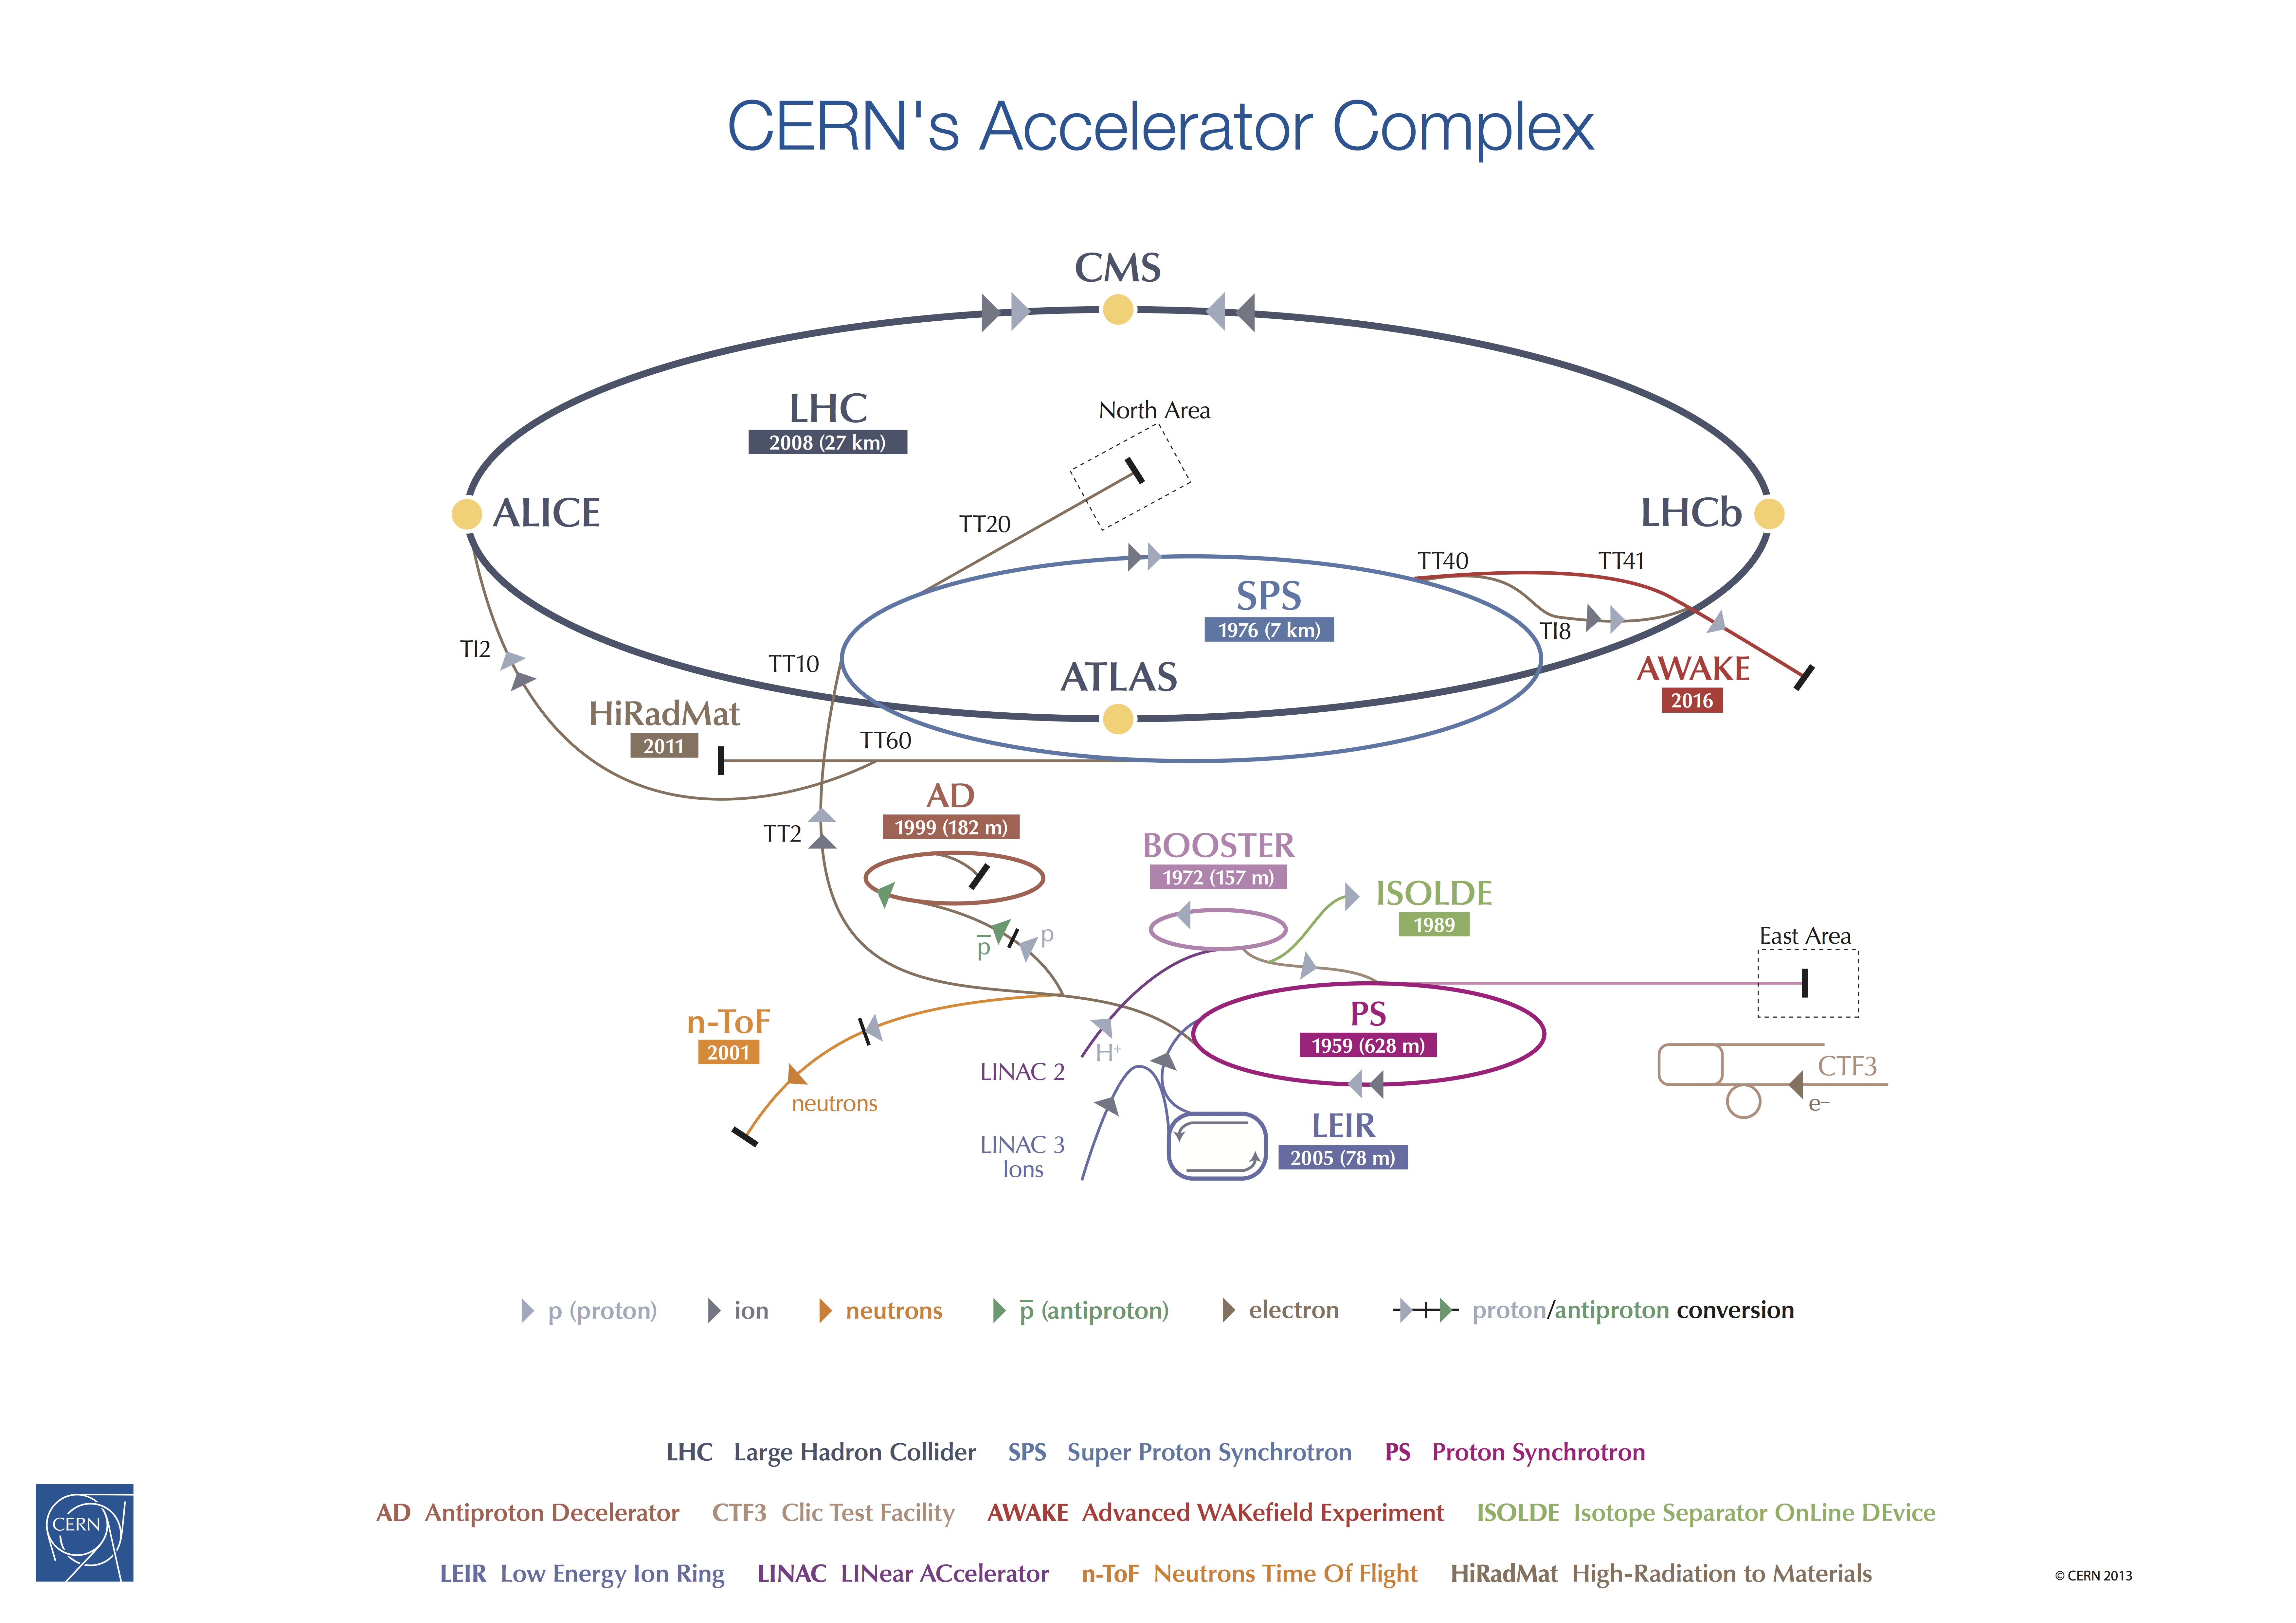
\includegraphics[width=\textwidth]{LHC/LHC_accelerator_complex.jpg}
 \caption{Sketch of the CERN accelerator complex.
  The LHC (dark grey ring) is the last ring in a complex chain of particle accelerators, where smaller machines are used in a chain to help boost particles to their final energies and provide beams to a whole set of smaller experiments~\cite{Haffner:1621894}.
  The LHC proton injector chain is the indicated by the paths marked with light grey arrows.}\label{fig:LHC_accelerator_complex}
\end{figure}

\section{Collider}

The circulating proton beams in the LHC cross paths at the four interaction points where the main LHC experiments are located.
The collisions of the proton beams in the experiments have a resulting center of mass energy of $\sqrt{s} = 13~\TeV$ and, as shown by \Cref{eq:events_from_luminosity}, the number of events generated per second for a particular process is governed by the machine (instantaneous) luminosity, $\luminosity$, which for a beam shape that is Gaussianly distributed is
\begin{equation}
 \luminosity = \frac{N_{b}^{2} n_{b} f_{\mathrm{rev}} \,\gamma_{r}}{4 \pi \epsilon_{n} \beta^{*}} F
 \label{eq:machine_luminosity}
\end{equation}
where $N_{b}$ is the number of particles per bunch, $n_{b}$ is the number of bunches per beam, $f_{\mathrm{rev}}$ is the revolution frequency, $\gamma_{r}$ is the relativistic gamma factor, $\epsilon_{n}$ is the normalized transverse beam emittance, $\beta^{*}$ is the beta function at the collision point, and $F$ is the geometric luminosity reduction factor due to the crossing angle at the interaction point:
\[
 F = \left(1 + \left(\frac{\theta_{c} \,\sigma_{z}}{2 \sigma^{*}}\right)\right)^{-1/2},
\]
where $\theta_{c}$ is the full crossing angle at the interaction point, $\sigma_{z}$ is the RMS bunch length, and $\sigma^{*}$ is the transverse RMS beam size at the interaction point~\cite{Evans:2008}.
Nominal design values for these quantities are given in \Cref{table:LHC_collider_parameters}, which additionally shows the incredibly successfully results of the LHC operations and accelerator teams' operation of the LHC in Run II.
From \Cref{eq:events_from_luminosity} and \Cref{eq:machine_luminosity} it is seen that to obtain the high number of hard collisions to have sensitivity to new physics both high beam energies and high luminosities are required.
As can be seen from \Cref{eq:machine_luminosity}, one approach to increasing the luminosity in the future for the High-Luminosity LHC (HL-LHC) is to decrease $\beta^{*}$ through the use of more powerful quadrupole focusing magnets.
However, this requires a larger crossing angle, decreasing the geometric factor, but this can be compensated for by the use of crab cavities~\cite{PhysRevAccelBeams.19.101003}.

\begin{table}[htpb]
 \centering
 \caption{Nominal design values of LHC operations parameters at ATLAS for $25~\textrm{ns}$ bunch crossing spacing~\cite{Evans:2008,PhysRevAccelBeams.19.101003}.
  Design and ATLAS recorded values of the machine luminosity are also given for LHC Run II operations~\cite{TWiki:2018ATLASPeakLumi}.
 }
 \begin{tabular}{@{}llr@{}} \toprule
  Parameter                                   & Symbol             & LHC Run II Value                     \\ \midrule
  LHC circumference                           &                    & $26,659~\mathrm{m}$                  \\
  LHC beam energy                             &                    & $7~\TeV$                             \\
  LHC beam energy in Run II                   &                    & $6.5~\TeV$                           \\
  Number of protons per bunch                 & $N_{b}$            & $1.15 \times 10^{11}$                \\
  Number of proton bunches per beam           & $n_{b}$            & $2,808$                              \\
  Revolution frequency                        & $f_{\textrm{rev}}$ & $11.245~\mathrm{kHz}$                \\
  Lorentz factor                              & $\gamma_{r}$       & $7462.69$                            \\
  Lorentz factor at $\sqrt{s} = 13~\TeV$      &                    & $6929.64$                            \\
  Normalized transverse beam emittance        & $\epsilon_{n}$     & $3.75~\mu\mathrm{m}$                 \\
  Collision point beta function               & $\beta^{*}$        & $0.55~\mathrm{m}$                    \\
  Full crossing angle                         & $\theta_{c}$       & $285~\mu\mathrm{rad}$                \\
  RMS bunch length                            & $\sigma_{z}$       & $7.55\times 10^{-2}~\mathrm{m}$      \\
  Transverse RMS beam size                    & $\sigma^{*}$       & $16.6~\mu\mathrm{m}$                 \\ \midrule
  Peak design machine luminosity at $14~\TeV$ & $\luminosity$      & $10~\mathrm{nb}^{-1}\mathrm{s}^{-1}$ \\
  Peak design machine luminosity at $13~\TeV$ &                    & $9~\mathrm{nb}^{-1}\mathrm{s}^{-1}$  \\
  Peak ATLAS recorded machine luminosity      &                    & $21~\mathrm{nb}^{-1}\mathrm{s}^{-1}$ \\
  \bottomrule
 \end{tabular}\label{table:LHC_collider_parameters}%
\end{table}


 \chapter{The ATLAS Experiment}\label{chapter:ATLAS}

\section{Overview}\label{sec:ATLAS_overview}

The ATLAS Experiment~\cite{PERF-2007-01} is one of the four main LHC experiments with the ATLAS detector, seen in \Cref{fig:ATLAS_detector}, located in the experiment cavern at Point 1 of the LHC roughly $100~\textrm{m}$ underground.
The ATLAS detector, henceforth also referred to as just ``ATLAS,'' is a general purpose, high luminosity particle physics detector designed to be able to search for as many types of interesting physics events as possible.
ATLAS is the largest of the LHC experiments with dimensions of $44~\mathrm{m}$ in length and $25~\mathrm{m}$ in height.

\begin{figure}[htbp]
 \centering
 \includegraphics[width=0.9\textwidth]{ATLAS/ATLAS_detector.eps}
 \caption[Cut-away view of the ATLAS detector.]{%
  Model of human particle physicists with ATLAS detector shown for scale~\cite{Pequenao:1095924}.}\label{fig:ATLAS_detector}
\end{figure}

\section{Geometry}\label{sec:ATLAS_geometry}

The ATLAS detector is cylindrical in design and forward-backward symmetrical with respect to the center of the detector.
The inner detector is surrounded by a $2~\mathrm{T}$ superconducting solenoid magnet and provides excellent tracking coverage in $\abs{\eta} < 2.5$.
The inner detector is further bracketed at each end by end-cap toroid magnets and the entire barrel of the detector out through the calorimeters is enclosed in a toroid magnet system.
These two toroid systems are both constructed such that they exhibit an eight-fold azimuthal symmetry.
As a result, almost all of ATLAS also exhibits this eight-fold axial symmetry, with the noted exception of the support structures on the bottom that support the detector off the ground.
The detectors subsytems, described in the following sections, are radially concentric and cover different pseudorapidity ranges, with the liquid-argon (LAr) forward calorimeters extending the coverage out to $\abs{\eta} = 4.9$.

\section{Tracking in the Inner Detector}\label{sec:ATLAS_ID}

Located at the heart of ATLAS and inside of the $2~\mathrm{T}$ solenoidal magnetic field, the \gls{inner detector} subsystem, seen in \Cref{fig:ATLAS_inner_detector}, provides precision tracking through the combined performance of successive layers of pixel detectors, silicon \gls{SCT}, and the straw tube \gls{TRT} and provides excellent coverage up to $\abs{\eta} < 2.5$.
To maximize the effective detector area, the pixels and SCT in the barrel region are arranged in concentric cylinders, as seen in \Cref{fig:ATLAS_pixel}.
The pixel layers are closest to the beamline and consist of roughly $80.4$ million identical pixel sensors forming three cylindrical layers in the barrel and three consecutive disks at each end-cap.
Each of the pixels is of area\footnote{$50~\mu\mathrm{m}$ in the $R\textrm{-}\phi$ direction by $400~\mu\mathrm{m}$ in the $z$ direction.} $20,000~\mu\mathrm{m}^{2}$ with resolution of $10~\mu\mathrm{m}~(R\textrm{-}\phi) \times 115~\mu\mathrm{m}~(z)$.
The excellent resolution in $R\textrm{-}\phi$ is a result of the strong magnetic field bending particles along $\hat{\vec{\phi}}$ causing them to spiral through the pixel detector~\cite{PERF-2007-01}.
Charged particle hits in the pixel detector are paramount for robust tracking and identifying and reconstructing the primary and secondary vertices necessary for physics object reconstruction (i.e., jets) and flavour tagging.

\begin{figure}[htbp]
 \centering
 \includegraphics[width=0.65\textwidth]{ATLAS/ATLAS_inner_detector.eps}
 \caption[Cut-away view of the ATLAS inner detector showing the pixel detector, Semiconductor Tracker, and Transition Radiation Tracker.]{%
  Cut-away view of the ATLAS inner detector showing the pixel detector, Semiconductor Tracker, and Transition Radiation Tracker~\cite{Pequenao:1095926}.}\label{fig:ATLAS_inner_detector}
\end{figure}

\begin{figure}[htbp]
 \centering
 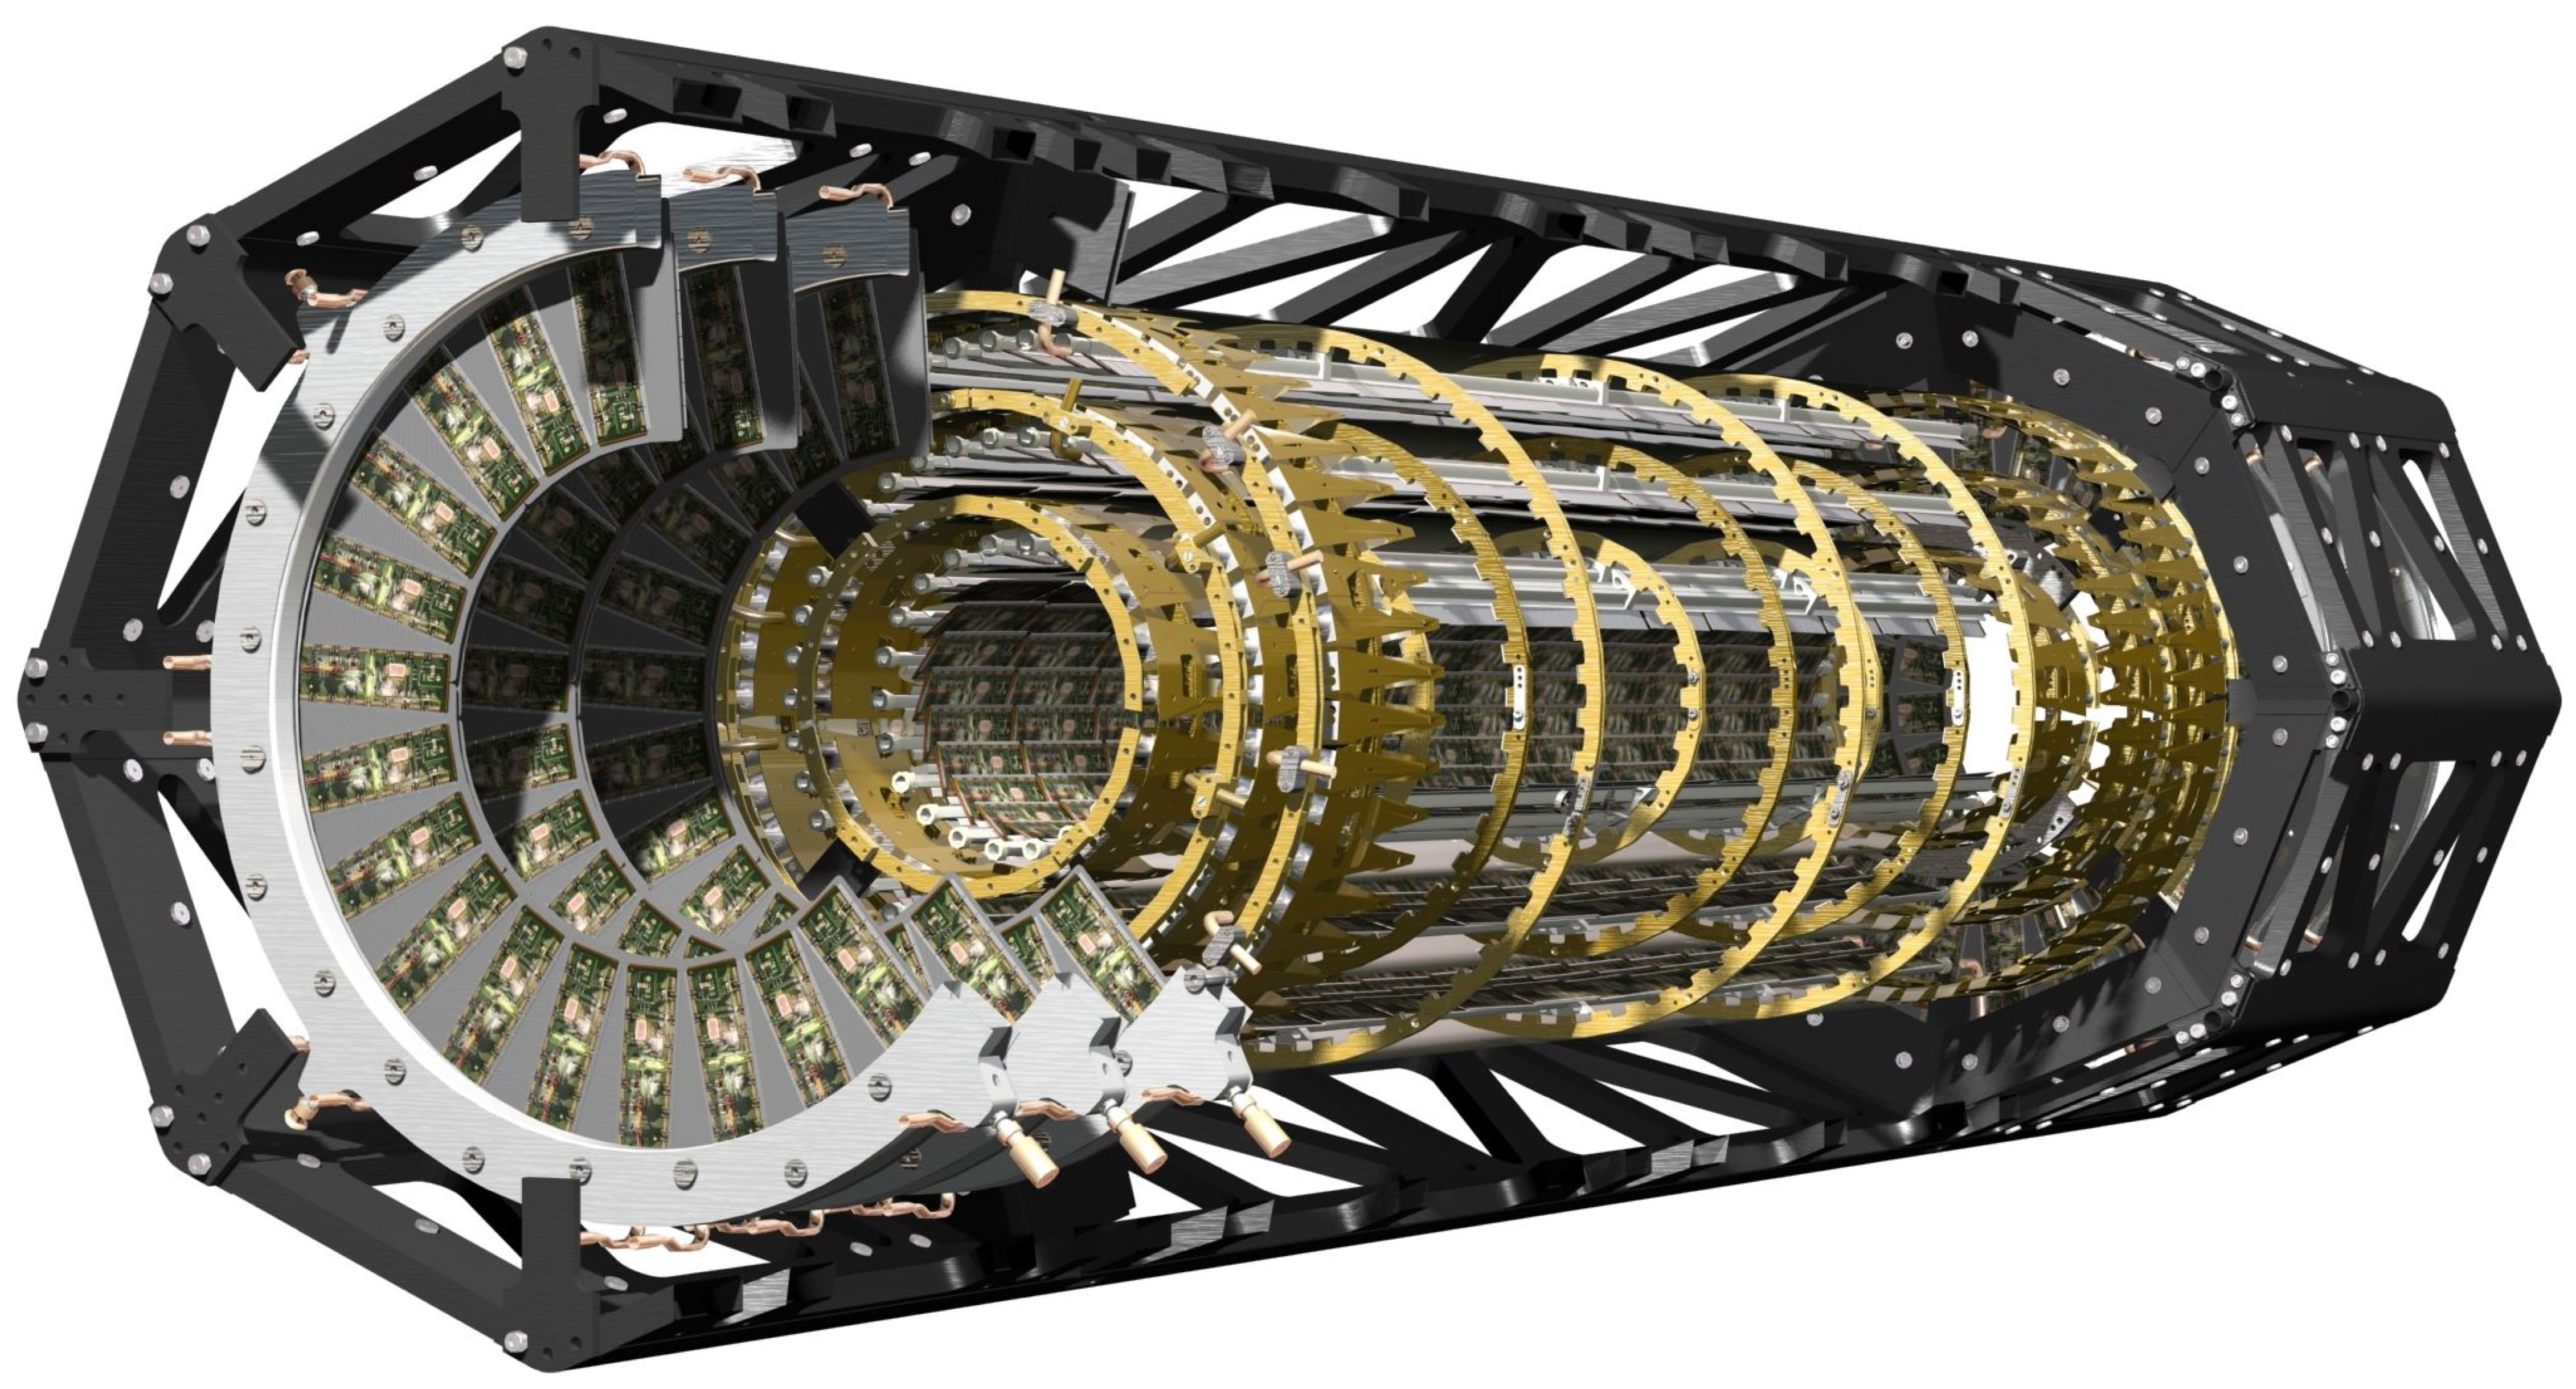
\includegraphics[width=0.6\textwidth]{ATLAS/ATLAS_pixel.eps}
 \caption[Cut-away view of the ATLAS pixel detector in the inner detector.]{%
  Cut-away view of the ATLAS pixel detector in the inner detector~\cite{Pequenao:1095925}.
  The pixel sensors form three cylindrical layers in the barrel and three consecutive disks at each end-cap.}\label{fig:ATLAS_pixel}
\end{figure}

The \Gls{SCT} surrounds the pixel detector in the barrel with four layers of stereo strips with small angle coverage $(40~\mathrm{mrad})$, shown in \Cref{fig:ATLAS_inner_detector_radial_view}, to measure hits in the silicon in both $R\textrm{-}\phi$ and $z$.
In the end-cap region, the SCT strips run radially in nine disks in each end-cap (for 18 disk in total).
In total, the SCT has roughly 6.3 million readout channels and results in track resolutions of $17~\mu\mathrm{m}~(R\textrm{-}\phi) \times 580~\mu\mathrm{m}~(z)$ in the barrel region and $17~\mu\mathrm{m}~(R\textrm{-}\phi) \times 580~\mu\mathrm{m}~(R)$ in the end-cap region.

The \Gls{TRT} further extends the ID $R\textrm{-}\phi$ information up to $\abs{\eta} = 2.0$ by providing a large number of track interactions with its approximately $351,000$ $4~\textrm{mm}$ straw tubes.
In the barrel region, the TRT straw tubes are parallel to the beam axis, shown in \Cref{fig:ATLAS_inner_detector_radial_view}, and extend for $144~\mathrm{cm}$ on either side of $\eta = 0$.
In the end-cap region, $37~\mathrm{cm}$ TRT straws are radially arranged with respect to the beamline in wheels, shown in \Cref{fig:ATLAS_inner_detector}.
Combined with the precision tracking from the pixel detectors and SCT, the tracking information that the TRT gives at larger radii contributes to high precision tracking of charged particles in both $R\textrm{-}\phi$ and $z$, and the large number of hits in the TRT significantly improve momentum measurements.

\begin{figure}[htbp]
 \centering
 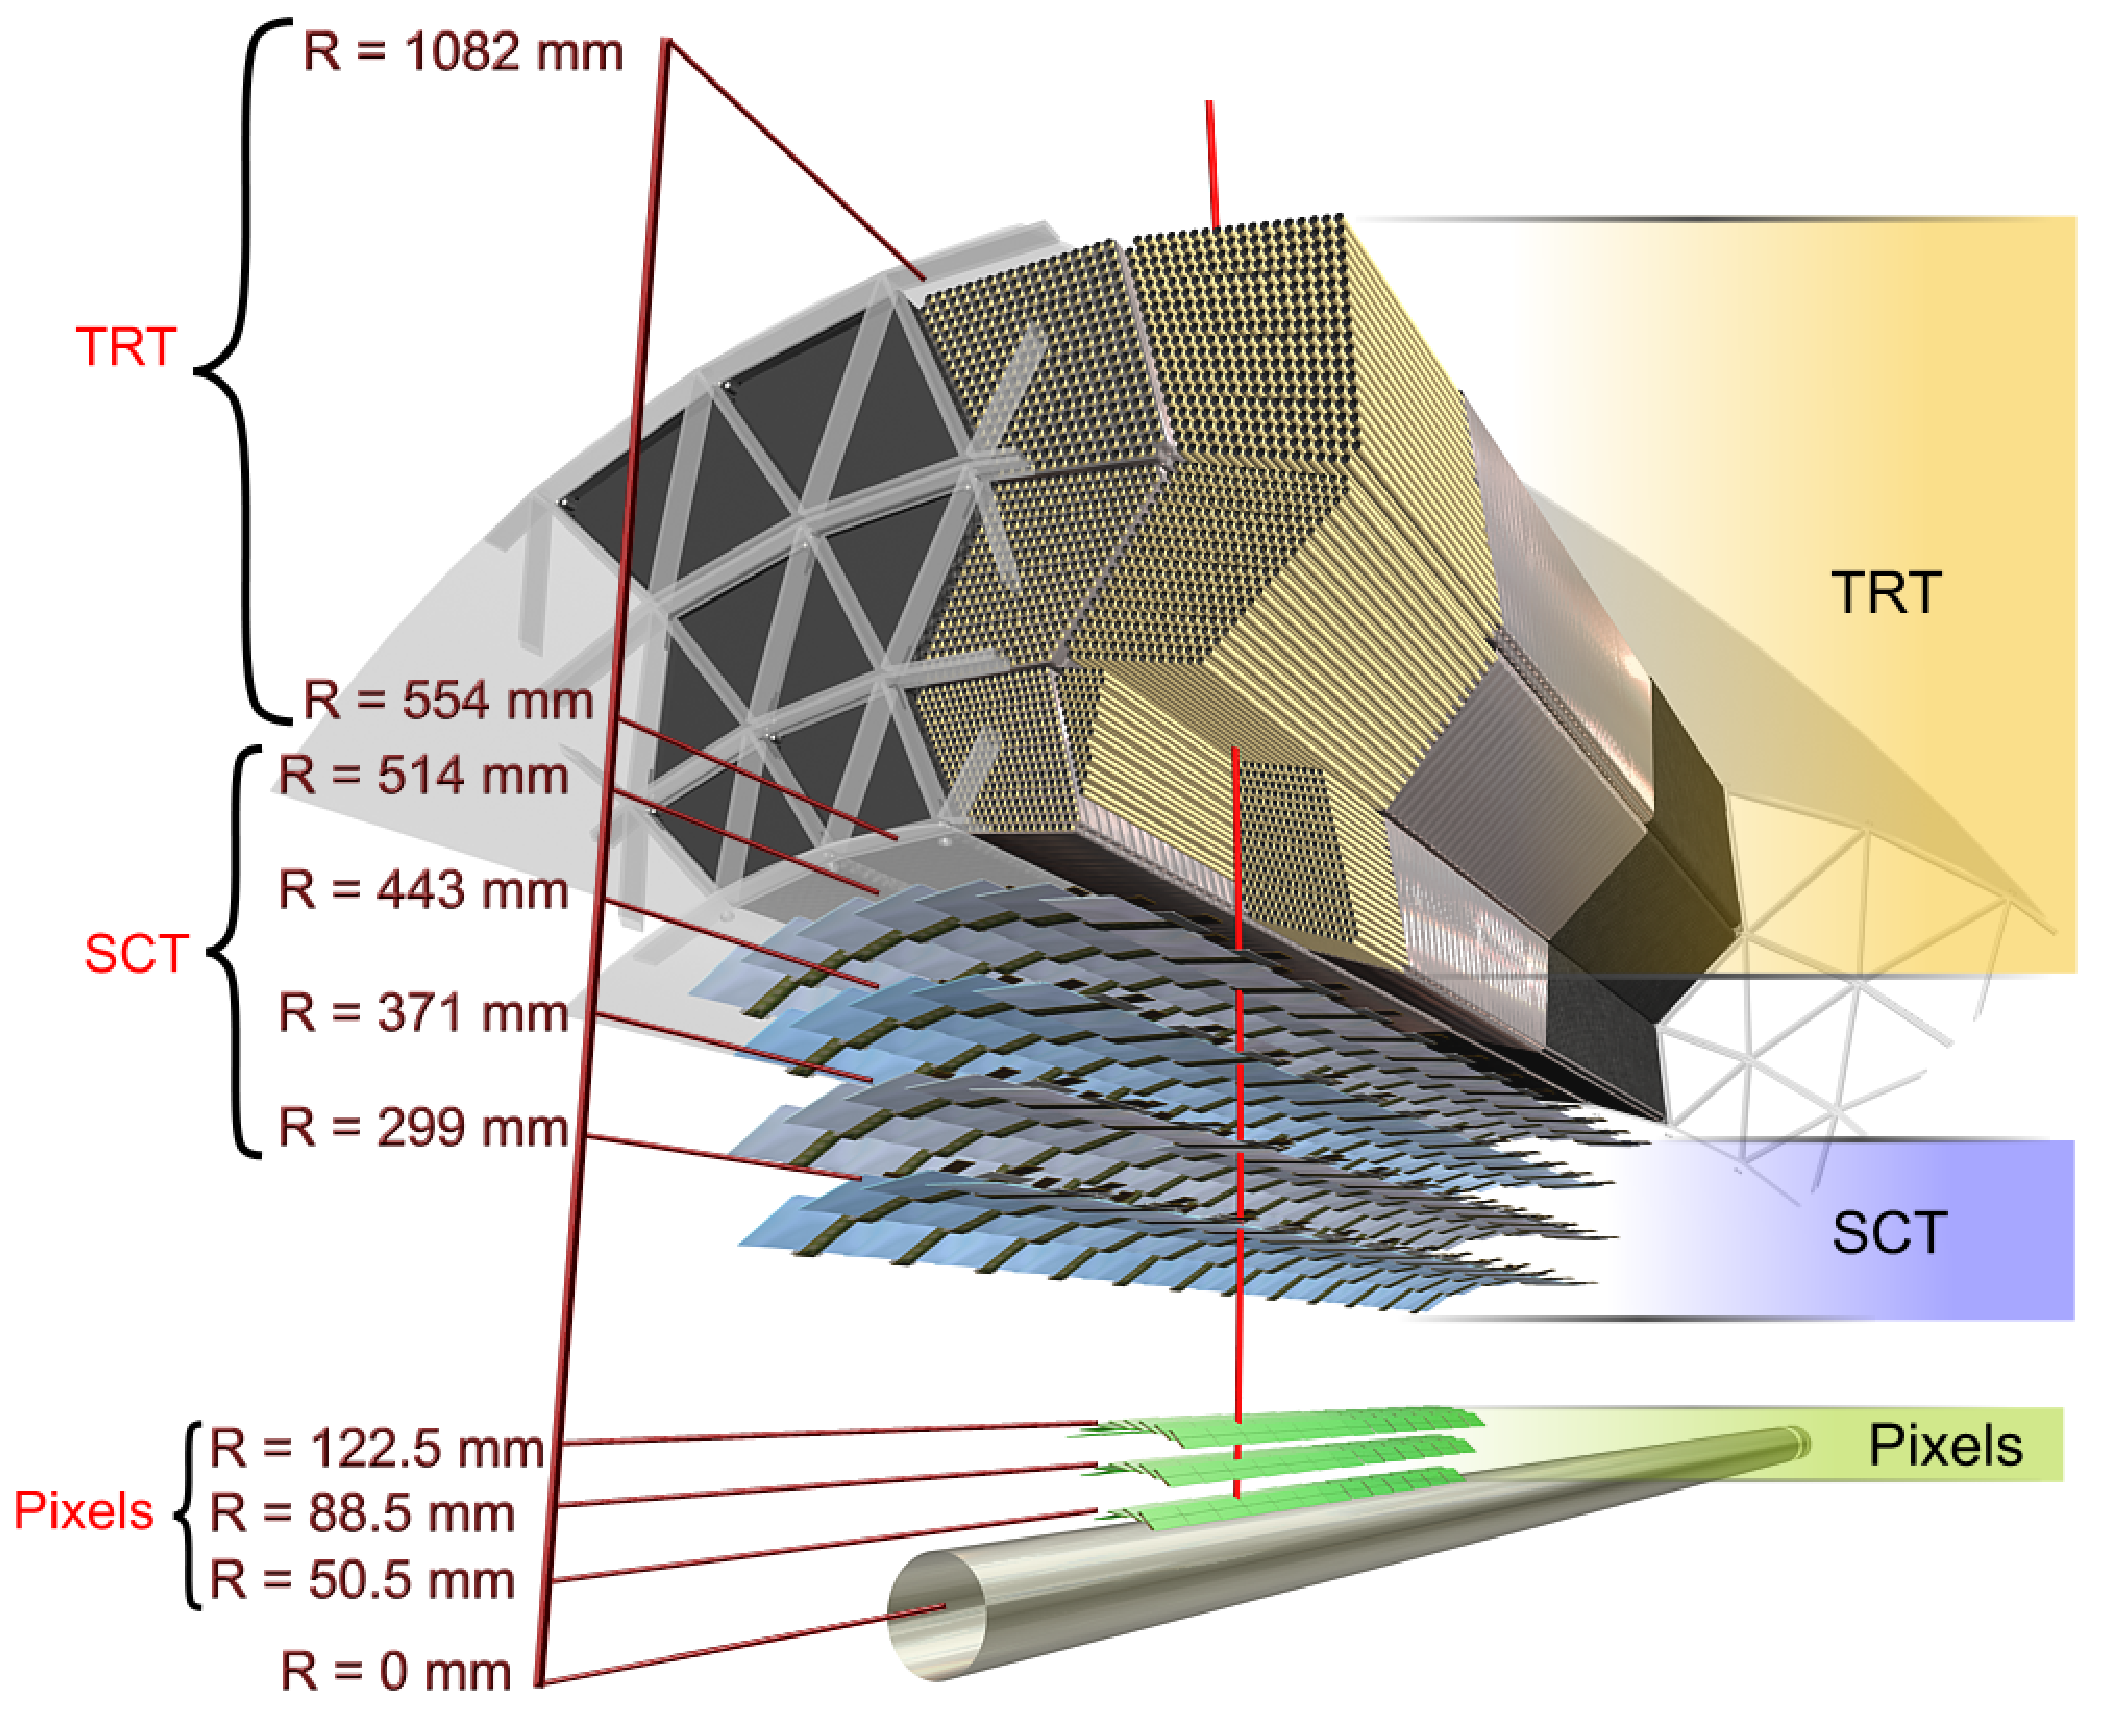
\includegraphics[width=0.6\textwidth]{ATLAS/ATLAS_inner_detector_radial_view.eps}
 \caption[Scale cut-away view of the pixel detector, Semiconductor Tracker, and Transition Radiation Tracker in the barrel-region.]{%
  The sensors and structural elements traversed by a charged track of $10~\GeV$ $p_{T}$ in the barrel inner detector $(\abs{\eta} = 0.3)$.
  The track traverses successively the beryllium beam-pipe, the three cylindrical silicon-pixel layers with individual sensor elements of $50 \times 400~\mu\mathrm{m}^{2}$, the four cylindrical double layers (one axial and one with a stereo angle of $40~\mathrm{mrad}$) of barrel SCT sensors of pitch $80~\mu\mathrm{m}$, and approximately 36 axial straws of $4~\mathrm{mm}$ diameter contained in the barrel TRT modules within their support structure~\cite{PERF-2007-01}.}\label{fig:ATLAS_inner_detector_radial_view}
\end{figure}

\section{Calorimeter System}\label{sec:ATLAS_calo}

The ATLAS calorimeter system, shown in \Cref{fig:ATLAS_calorimeter}, provides excellent energy deposition measurements for particles with coverage up to $\abs{\eta} < 4.9$ with different calorimetry subsystems for various physics processes.
In the pseudorapidity range of the inner detector ($\abs{\eta} < 2.5$) the high granularity electromagnetic (EM) liquid argon calorimeter system provides measurement of electrons and photons.
The more coarse resolution of the hadronic calorimeter systems provides measurements for jet reconstruction and missing transverse momentum, $\MET$, in conjunction with the large pseudorapidity coverage.
These calorimeter designs are both ``sampling calorimeters'', where the ``active'' materials that provide the signals are different from the ``absorber'' materials that reduce the particle energy and cause showering.
The calorimeter subsystems are also designed to be sufficiently thick as to contain the electromagnetic and hadronic showers that originate inside them, and to limit punch-through to the muon systems.

\begin{figure}[htbp]
 \centering
 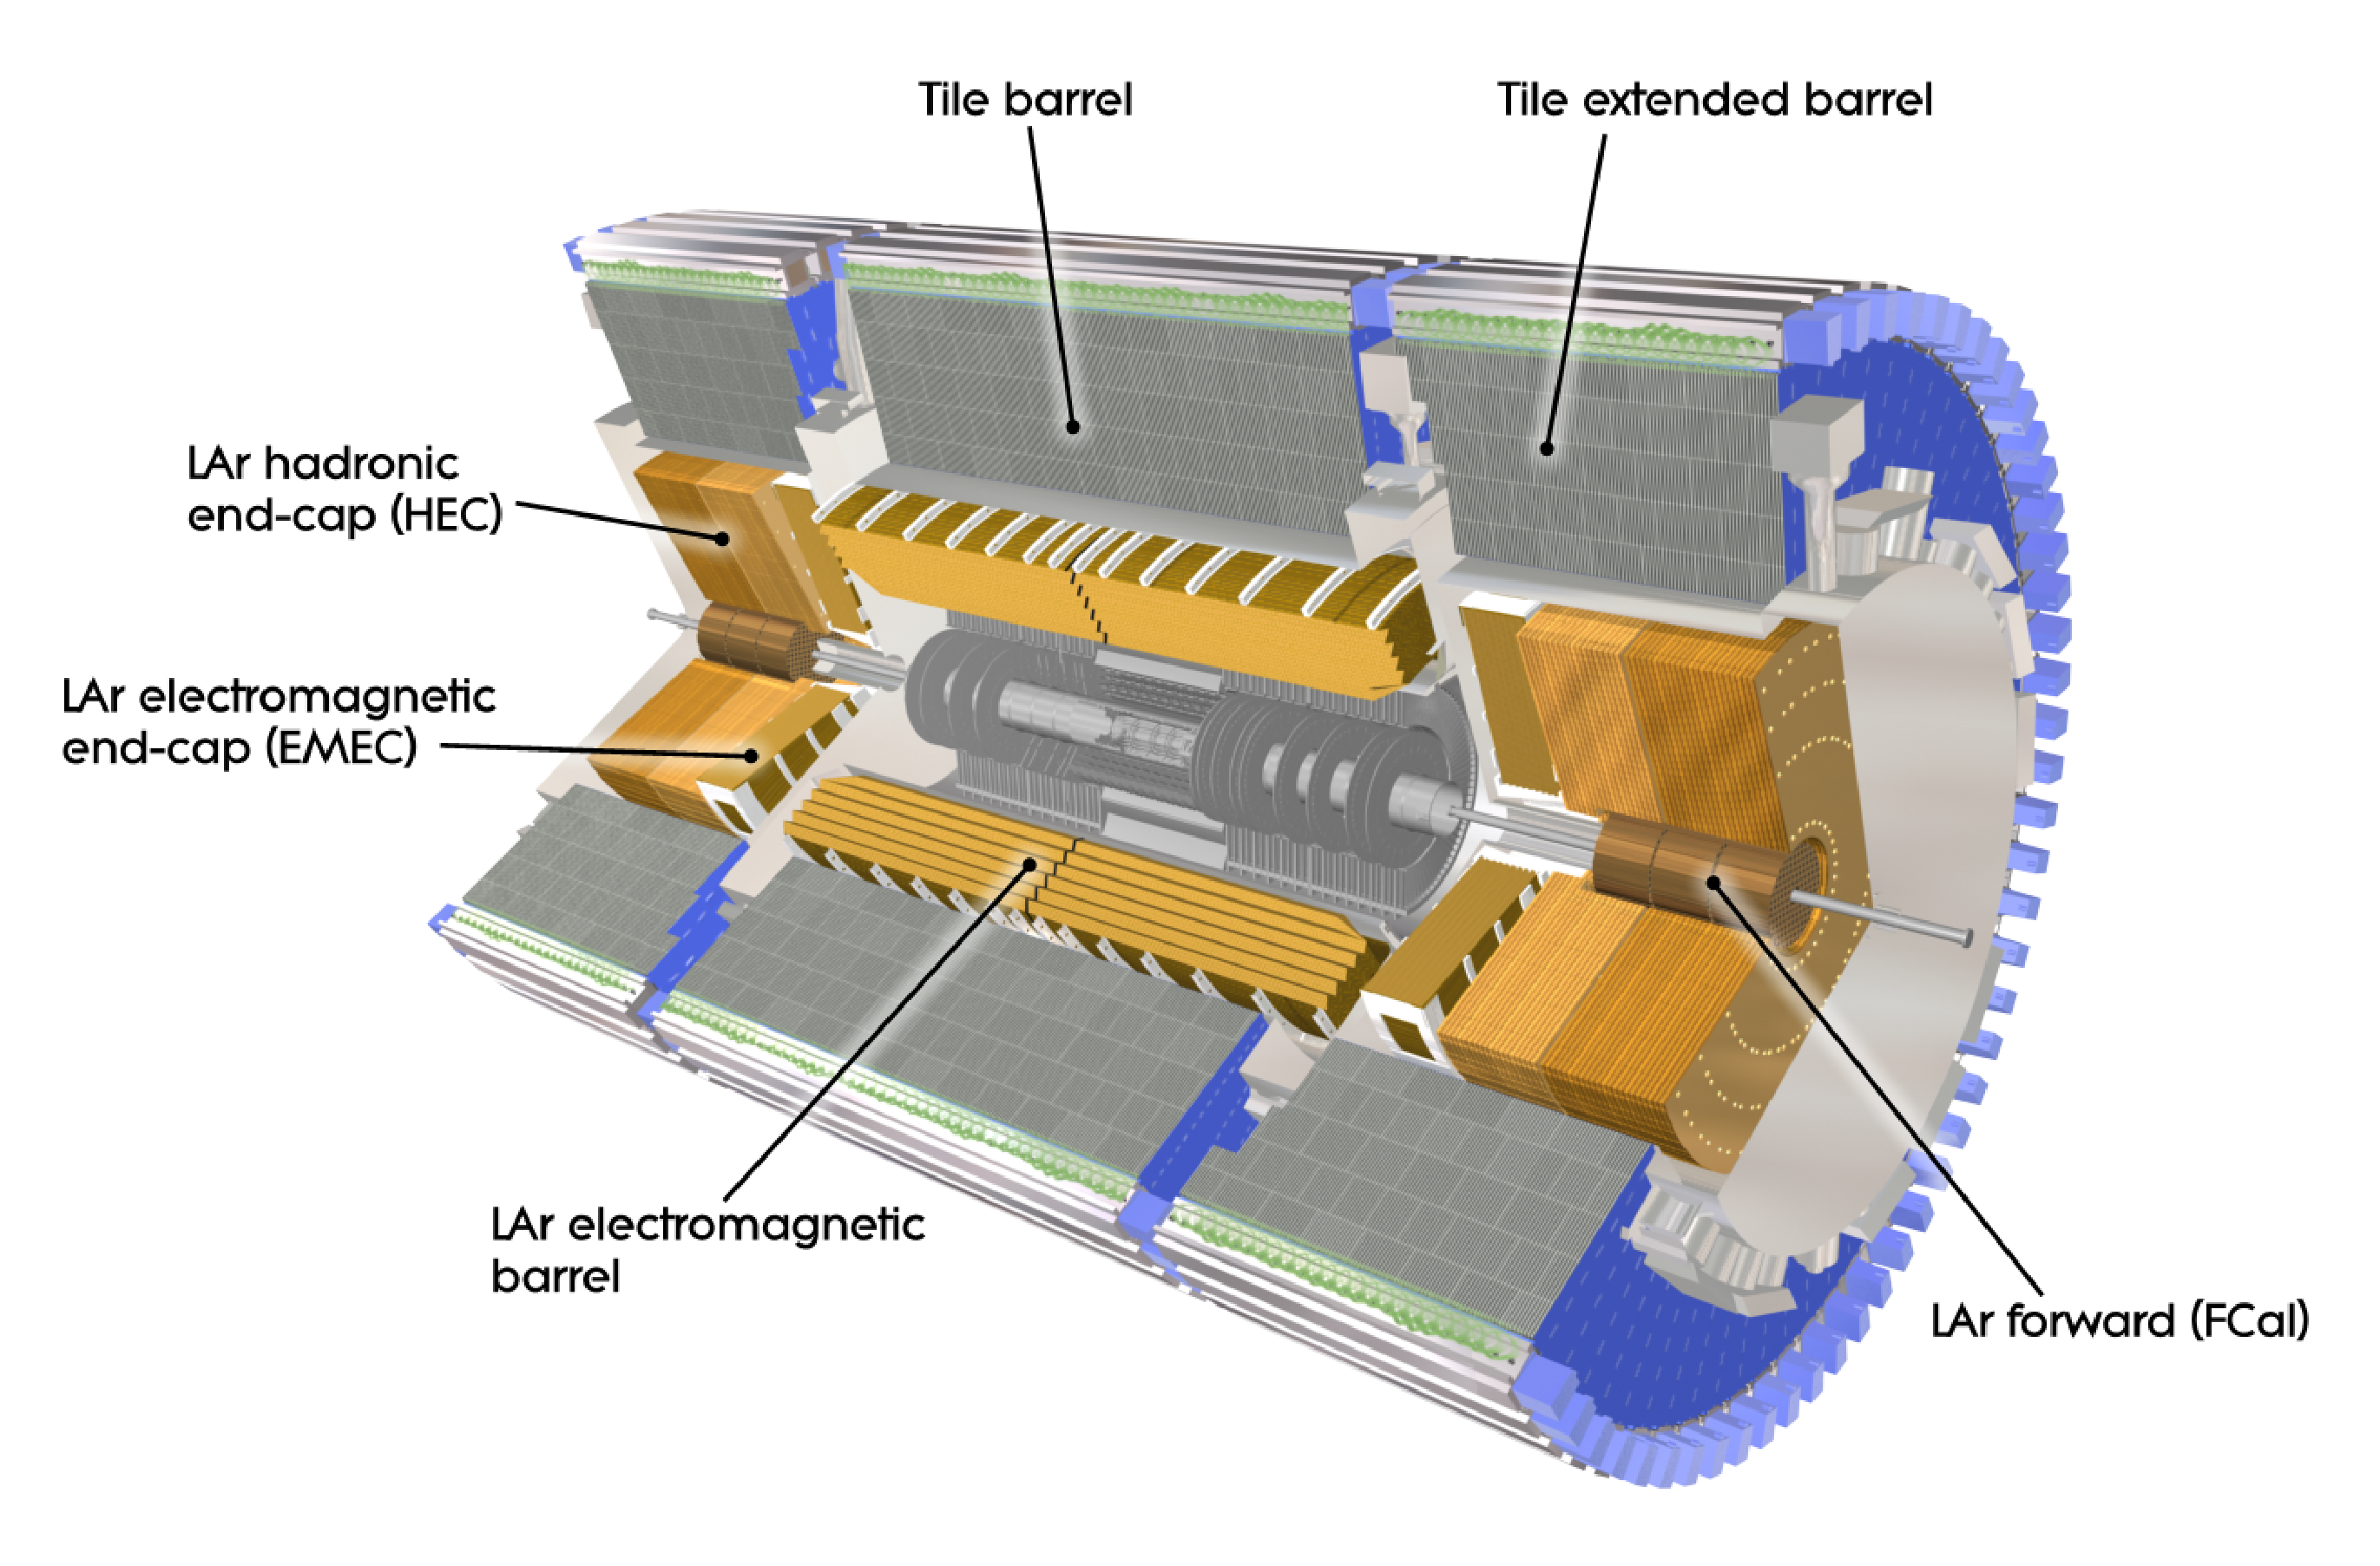
\includegraphics[width=0.7\textwidth]{ATLAS/ATLAS_calorimeter.eps}
 \caption[Cut-away view of the ATLAS calorimeter system.]{%
  Cut-away view of the ATLAS calorimeter system~\cite{Pequenao:1095927}.}\label{fig:ATLAS_calorimeter}
\end{figure}

\subsection{Electromagnetic Calorimeter}\label{sec:ATLAS_electromagnetic_calorimeter}

The electromagnetic calorimeter system, shown in \Cref{fig:ATLAS_LAr}, consists of lead-liquid argon detectors with a characteristically unique ``accordion'' lead absorber plate design that allows for continuous coverage in $\phi$ with folding angles of the accordion ``waves'' that vary with the radius to keep the LAr gap constant, as shown in \Cref{fig:ATLAS_LAr_module}.
Liquid argon (LAr) is the active detector material for the EM calorimeters as it has a linear behavior, very stable response over time, and is intrinsically radiation-hard.
In the barrel region the LAr EM calorimeter is split into symmetric half-barrels, and in the end-caps the LAr EM calorimeter exists as two coaxial wheels, respectively covering the regions of $1.375 < \abs{\eta} < 2.5$ and $2.5 < \abs{\eta} < 3.2$.

\begin{figure}[htbp]
 \centering
 \includegraphics[width=0.7\textwidth]{ATLAS/ATLAS_LAr.jpg}
 \caption[Cut-away view of the ATLAS electromagnetic liquid argon calorimeter system.]{%
  Cut-away view of the ATLAS electromagnetic liquid argon calorimeter system~\cite{Pequenao:1095927}.}\label{fig:ATLAS_LAr}
\end{figure}

\begin{figure}[htbp]
 \centering
 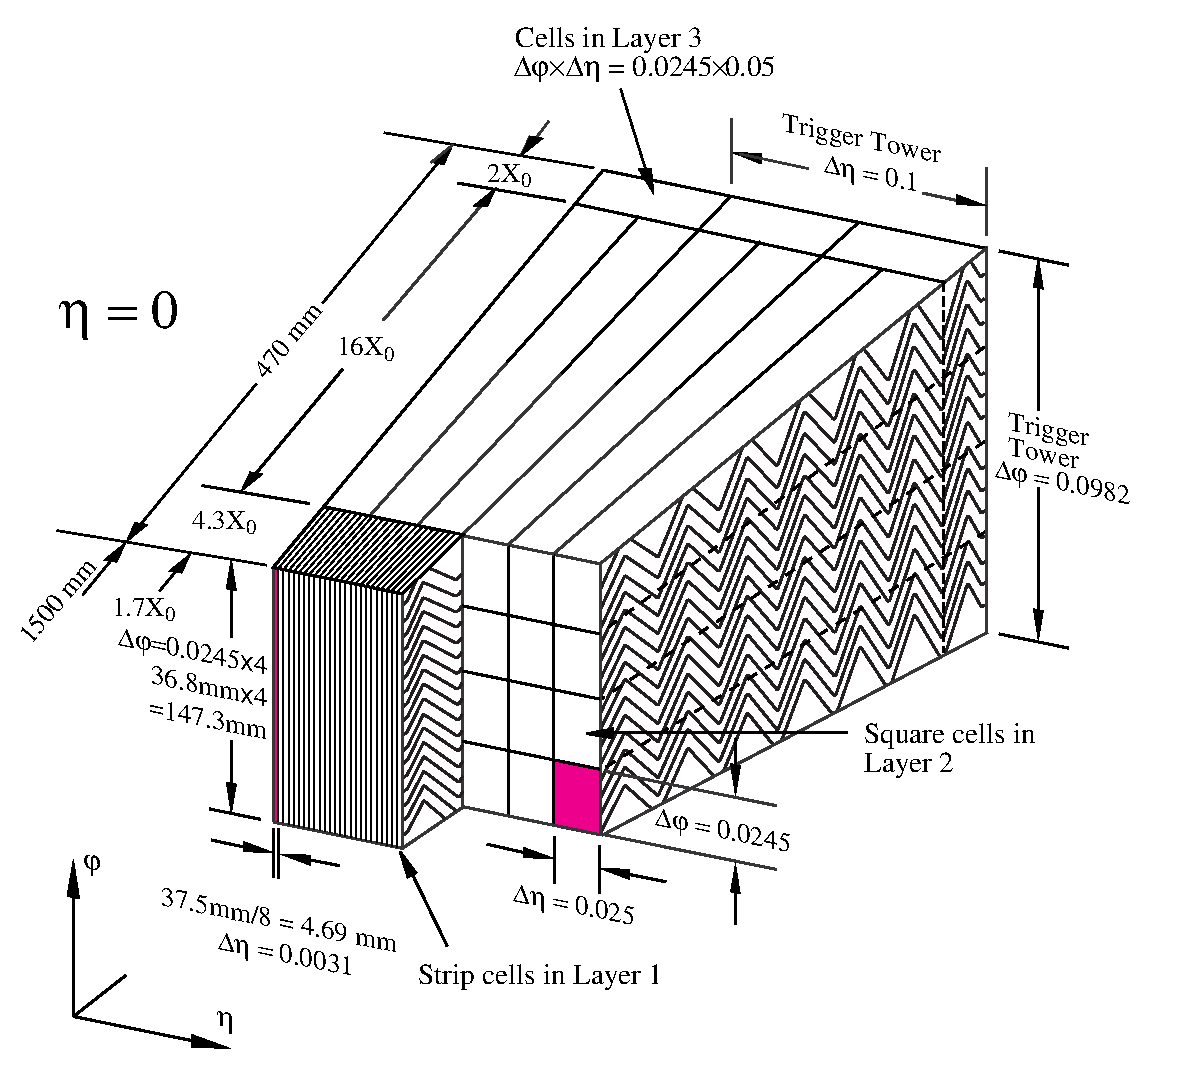
\includegraphics[width=0.6\textwidth]{ATLAS/ATLAS_LAr_module.eps}
 \caption[Sketch of a liquid argon calorimeter system barrel module detailing granularity in $\eta$ and $\phi$.]{%
  Sketch of a barrel module where the different layers are clearly visible with the ganging of electrodes in $\phi$.
  The granularity in $\eta$ and $\phi$ of the cells of each of the three layers and of the trigger towers is also shown~\cite{PERF-2007-01}.}\label{fig:ATLAS_LAr_module}
\end{figure}

\subsection{Hadronic Calorimeter}\label{sec:ATLAS_hadronic_calorimeter}

The hadronic calorimeter system is composed of the tile calorimeters in the barrel region, and the LAr Hadronic End-cap Calorimeter (HEC) and LAr Forward Calorimeter (FCal) in the end-cap region.
The tile sampling calorimeter resides outside the EM calorimeter system and provides coverage out to $\abs{\eta} < 1.7$ and radial coverage from $2.28~\mathrm{m}$ out to $4.25~\mathrm{m}$.
The tile calorimeter absorber material is steel and uses scintillating tiles as the active material, which are read out using wavelength shifting fibers into photomultiplier tubes.
The HEC exists as two wheels in each end-cap behind the end-cap EM calorimeter, extending the coverage in the end-caps out to $\abs{\eta} < 3.2$.
The copper absorber plates of the HEC are interleaved with $8.5~\mathrm{mm}$ spacers of LAr providing active material.
The FCal extends coverage from $3.1 < \abs{\eta} < 4.9$ and is composed of three modules in each end-cap: a copper module optimized for electromagnetic measurements, and then two made of tungsten for hadronic interaction measurements.
The modules are a metal matrix with regularly spaced longitudinal channels consisting of tubes with a concentric rod and LAr filling the gap between them.

For calorimetry systems the energy resolution improves as the energy of the particle, $E$ increases, generally as $1/\sqrt{E}$.
More specifically, the energy resolution, $\sigma\left(E\right)$, of a calorimeter is given as the quadratic sum\footnote{That is, $a \oplus b = \sqrt{a^{2} + b^{2}}$.}
\begin{equation}
 \frac{\sigma\left(E\right)}{E} = \frac{a}{\sqrt{E}} \oplus \frac{b}{E} \oplus c\,,
 \label{eq:calorimeter_energy_resolution}
\end{equation}
where $a$ is the ``stochastic term'' for intrinsic shower fluctuations, $b$ is the ``noise term'', and $c$ is the ``constant'' term~\cite{Fabjan:692252}.
It is seen from \Cref{eq:calorimeter_energy_resolution} that at lower energies the stochastic term is more important and at higher energies the constant term affects the energy resolution more.
The ATLAS calorimeters are designed to have excellent energy resolution, which is clearly seen from the observed energy resolution for the ATLAS LAr EM calorimeter barrel region in testbeam experiments~\cite{Ilic:2014,Aleksa:1547314}
\[
 \frac{\sigma\left(E\right)}{E} = \frac{10\%}{\sqrt{E}} \oplus \frac{200~\MeV}{E} \oplus 0.2\%\,.
\]
For the hadronic calorimeters the stochastic term is required to be under $50\%$ and the constant term under $3\%$~\cite{Ilic:2014}.

\section{Muon Spectrometer}\label{sec:ATLAS_muon_spectrometer}

The ATLAS muon spectrometer, shown in \Cref{fig:ATLAS_muon_spectrometer}, is arranged as the exterior detector subsystem to provide coverage for muons deflected from the air-core toroid magnets.
As muons are minimum ionizing particles%
\footnote{The mass stopping power for muons in the typical energy ranges at the LHC is less than $4~\MeV\,\mathrm{cm}^{2}/\mathrm{g}$.
 To put this in context, a $1~\GeV$ muon can punch through roughly $1~\mathrm{m}$ of iron before stopping~\cite{Garutti:lecture}.}
, as seen in \Cref{fig:Bethe-Bloch_stopping_power}, they pass through the inner detector and calorimeter systems while being radially deflected by the solenoid magnetic field before entering the toroidal magnetic field and getting deflected along $\hat{\vec{z}}$.
Given the resulting trajectories, in the barrel region muon tracks are measured by three cylindrical layers of \glspl{MDT}, shown in \Cref{fig:ATLAS_MDT_chamber} and \Cref{fig:ATLAS_muon_barrel_track}, and in the end-caps region three planes of MDT wheels before escaping the detector altogether --- hence the name \emph{spectrometer}.
For most of the $\eta$ range the MDTs perform most of the precision measurements of the tracks, though from $2 < \abs{\eta} < 2.7$ higher granularity \glspl{CSC} provide tracking to withstand the intense rate and radiation~\cite{PERF-2007-01}.

\begin{figure}[htbp]
 \centering
 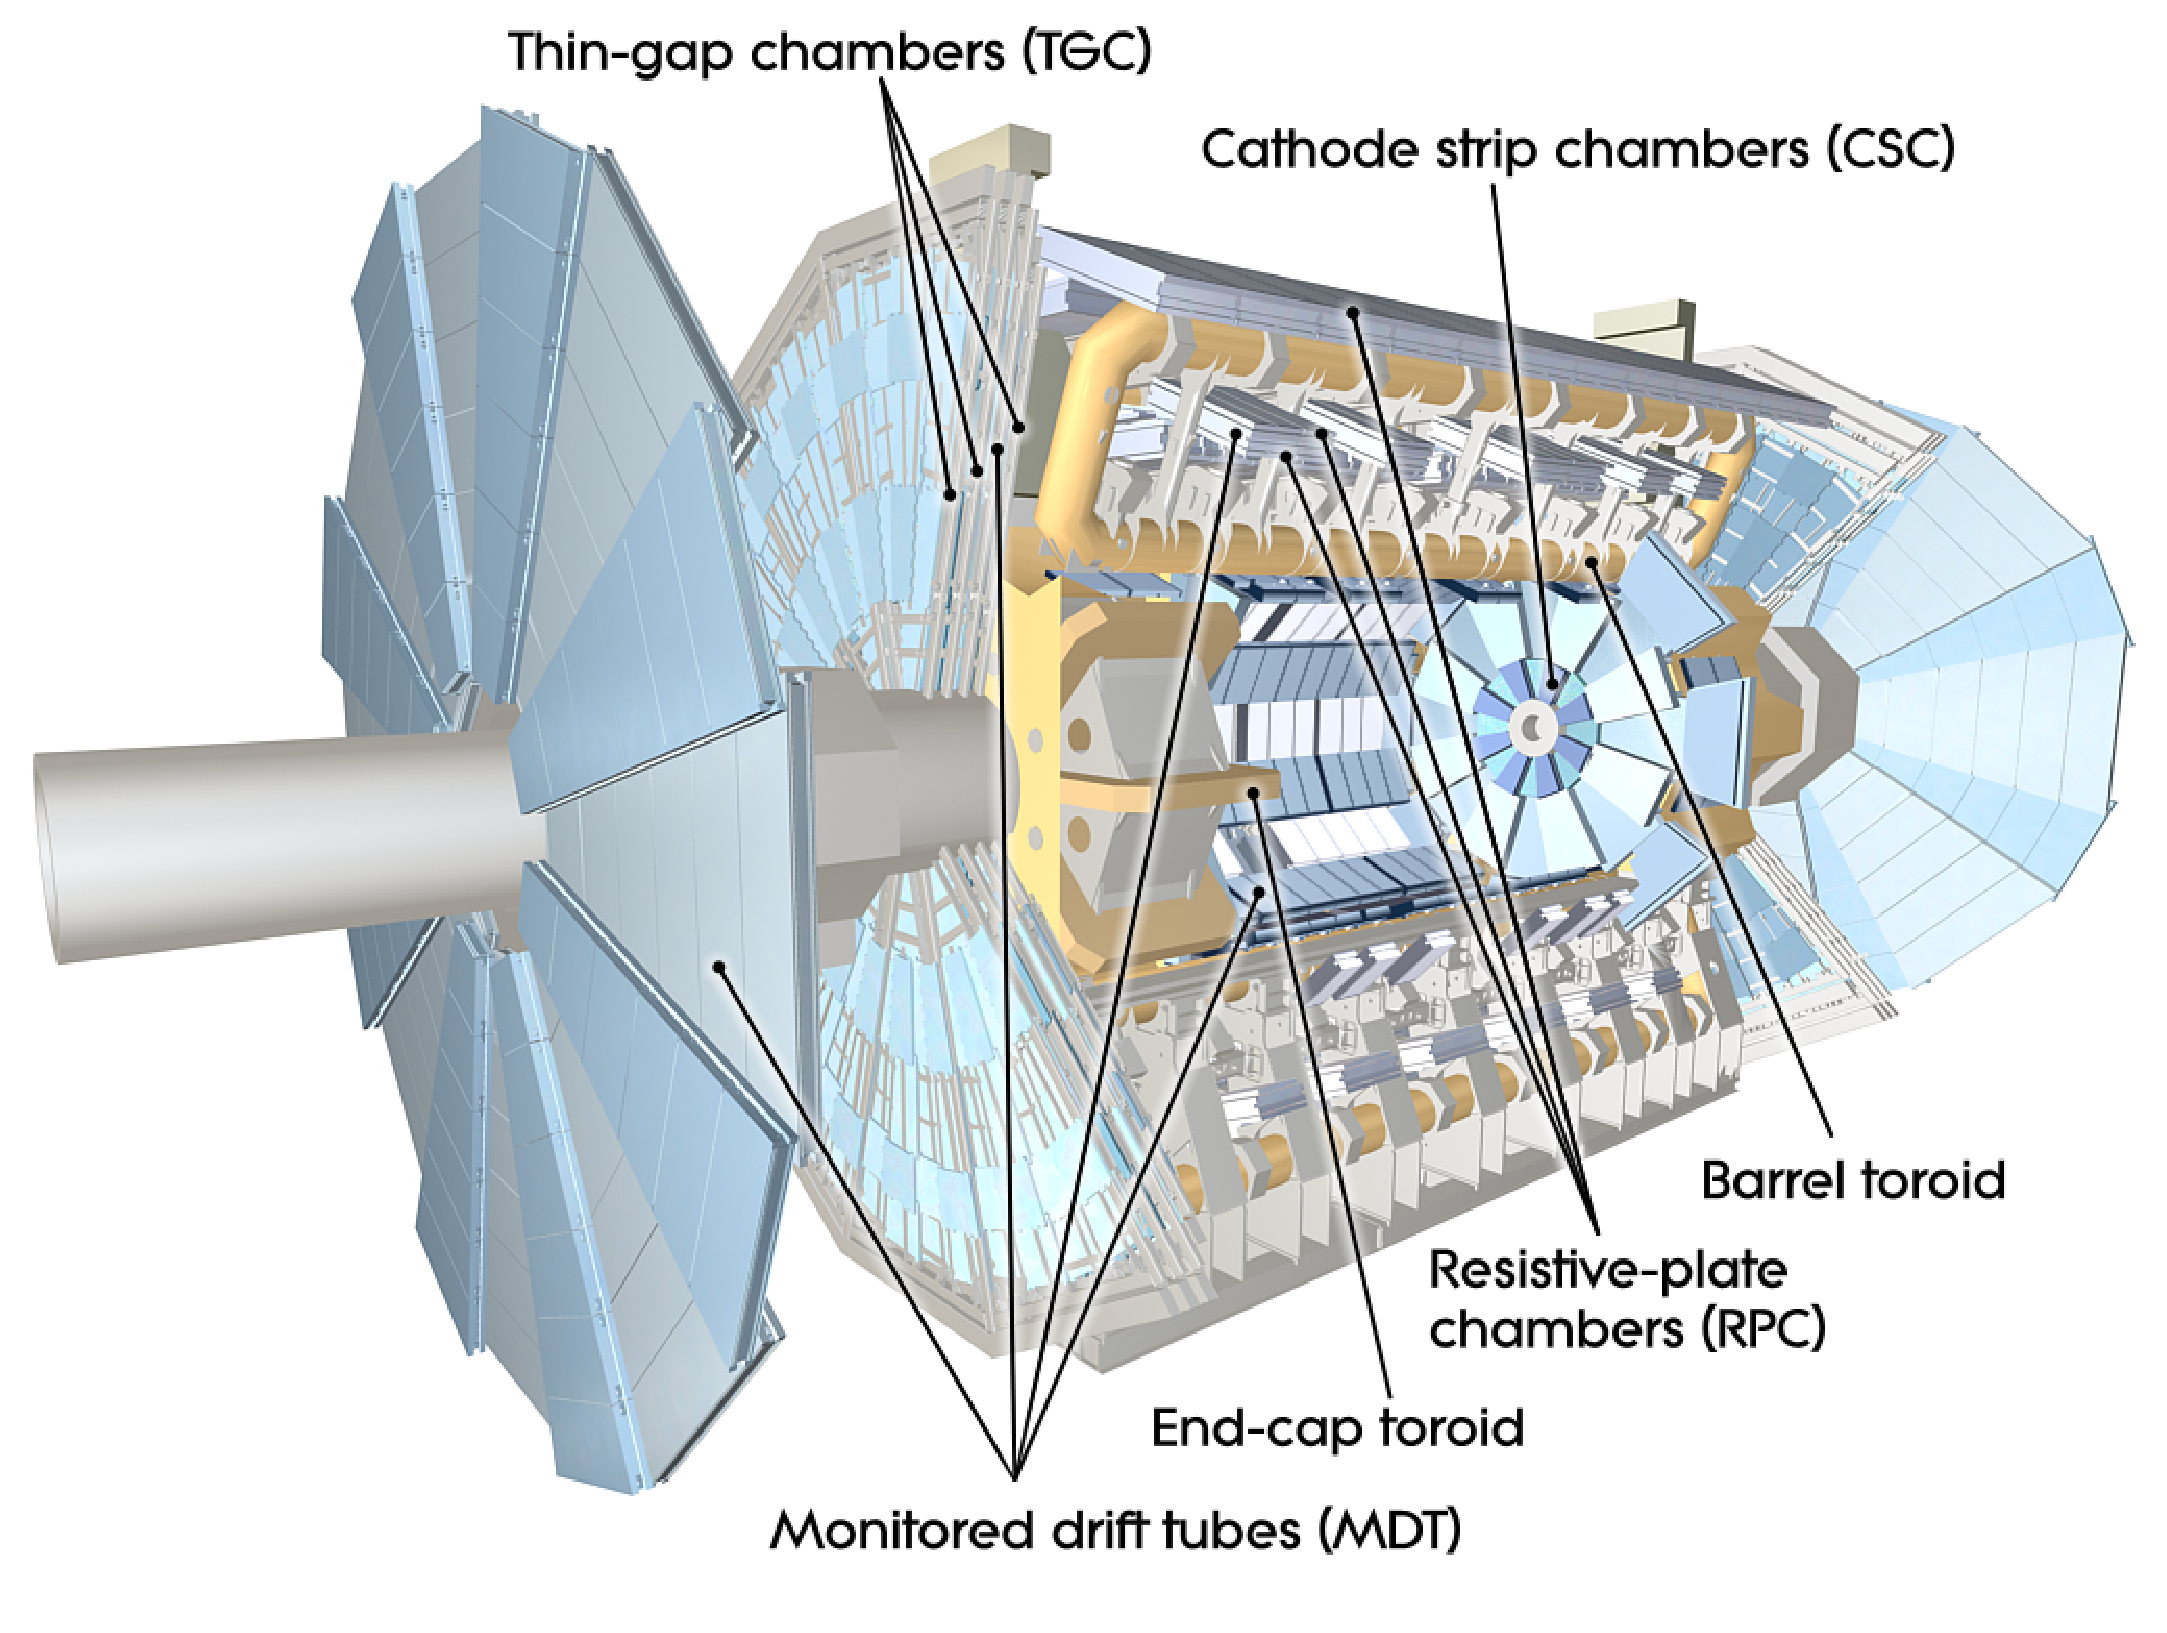
\includegraphics[width=0.6\textwidth]{ATLAS/ATLAS_muon_spectrometer.eps}
 \caption[Cut-away view of the ATLAS muon system.]{%
  Cut-away view of the ATLAS muon system~\cite{PERF-2007-01}.}\label{fig:ATLAS_muon_spectrometer}
\end{figure}

\begin{figure}[htbp]
 \centering
 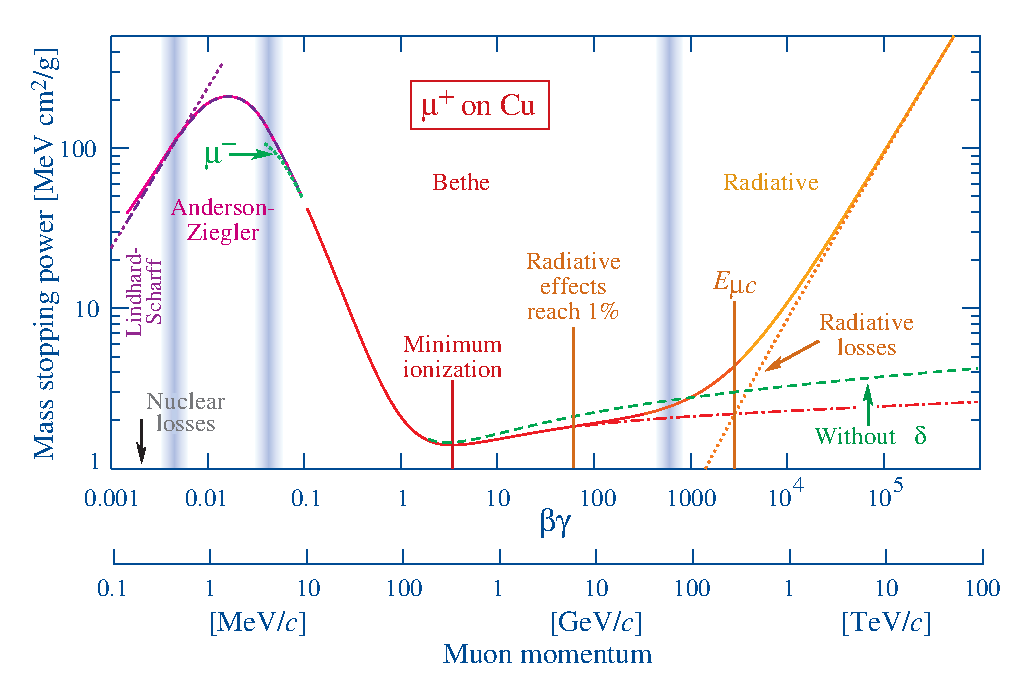
\includegraphics[width=\textwidth]{ATLAS/Bethe-Bloch_stopping_power.eps}
 \caption[Mass stopping power for positive muons in copper as a function of $\beta \gamma = p/Mc$.]{%
  Mass stopping power $\left(= \left<-dE/dx\right>\right)$ for positive muons in copper as a function of $\beta \gamma = p/Mc$ over nine orders of magnitude in momentum (12 orders of magnitude in kinetic energy).
  Solid curves indicate the total stopping power.
  Data below the break at $\beta \gamma \approx 0.1$ are taken from ICRU 49~\cite{ICRU49}, and data at higher energies are from~\cite{Groom:2001kq}.
  Vertical bands indicate boundaries between different approximations discussed in~\cite{PDG2018:Ch33}.
  The short dotted lines labeled ``$\mu^{-}$'' illustrate the ``Barkas effect'', the dependence of stopping power on projectile charge at very low energies~\cite{PhysRev.101.778}.
  $dE/dx$ in the radiative region is not simply a function of $\beta$~\cite{PDG2018:Ch33}.}\label{fig:Bethe-Bloch_stopping_power}
\end{figure}

\begin{figure}[htbp]
 \centering
 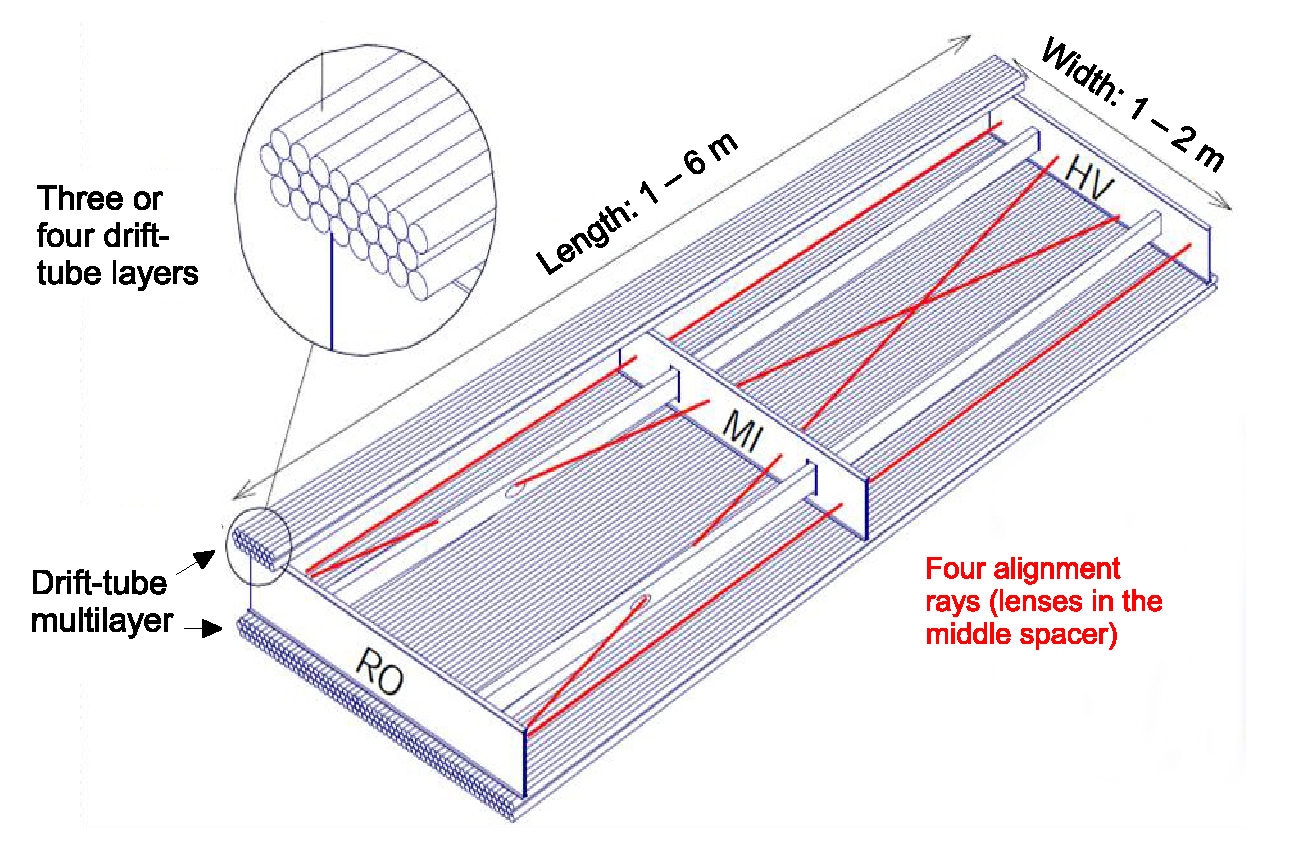
\includegraphics[width=0.6\textwidth]{ATLAS/ATLAS_MDT_chamber.eps}
 \caption[Mechanical structure of a \acrlong{MDT} chamber.]{%
  Mechanical structure of a \gls{MDT} chamber.
  Three spacer bars connected by longitudinal beams form an aluminium space frame, carrying two multi-layers of three or four drift tube layers.
  Four optical alignment rays, two parallel and two diagonal, allow for monitoring of the internal geometry of the chamber.
  RO and HV designate the location of the readout electronics and high voltage supplies, respectively~\cite{PERF-2007-01}.}\label{fig:ATLAS_MDT_chamber}
\end{figure}

\begin{figure}[htbp]
 \centering
 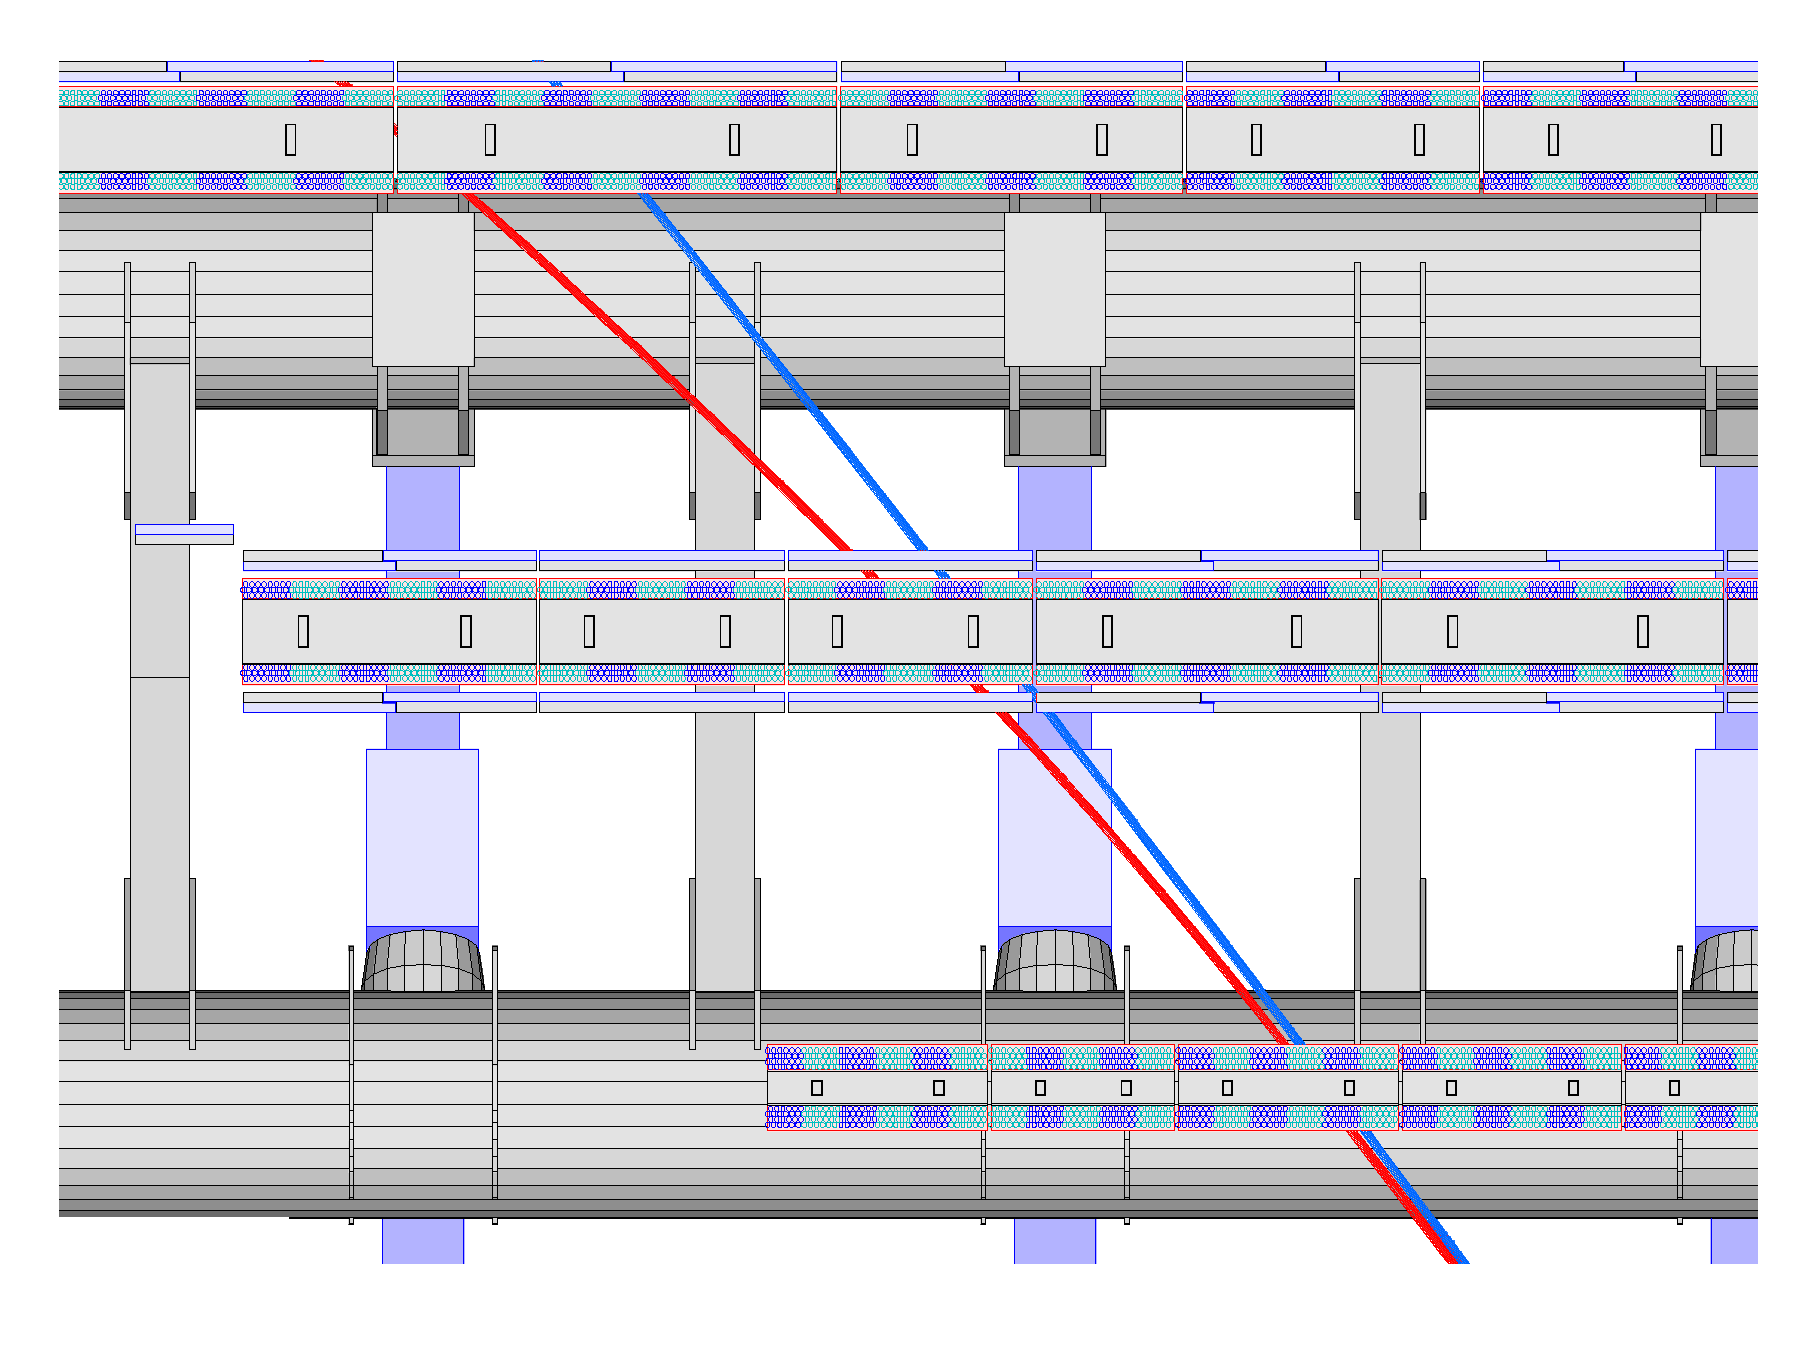
\includegraphics[width=0.6\textwidth]{ATLAS/ATLAS_muon_barrel_track.eps}
 \caption[Trajectories of muons through the three layers of \acrlong{MDT} of the barrel muon spectrometer.]{%
  Trajectories of muons with momenta of $4~\GeV$ and $20~\GeV$ in the bending plane of the barrel muon spectrometer.
  In general, the tracks cross $2 \times 4$ inner, $2 \times 3$ middle, and $2 \times 3$ outer layers of \gls{MDT} tubes.
  The cyan and dark blue areas in each MDT layer illustrate the granularity of the mezzanine cards~\cite{PERF-2007-01}.}\label{fig:ATLAS_muon_barrel_track}
\end{figure}

The trigger system for the muon system provides coverage out to $\abs{\eta} < 2.4$ and the \gls{RPC} and \gls{TGC} trigger chambers uniquely provide bunch-crossing identification, well-defined $p_{T}$ thresholds, and measurements of the muon track coordinate in the orthogonal direction of the precision-tracking chambers~\cite{PERF-2007-01}.

\section{Trigger and Data Acquisition}\label{sec:ATLAS_TDAQ}

The ATLAS \gls{TDAQ} systems, shown in \Cref{fig:ATLAS_TDAQ_system}, function collectively at two different levels: the L1 trigger and the \gls{HLT}.
Collectively, the trigger system is responsible for reducing the $40~\mathrm{MHz}$ event rate from the $25~\mathrm{ns}$ bunch crossings --- which is not possible to write out and save in real time --- to a much more manageable $1~\mathrm{kHz}$ that can be written to storage~\cite{TRIG-2016-01}.
With raw event sizes of approximately $1.6~\mathrm{Mbytes}$ this still results in data generation of over a Gigabyte per second.

\begin{figure}[htbp]
 \centering
 \includegraphics[width=\textwidth]{ATLAS/ATLAS_TDAQ_system.pdf}
 \caption[The ATLAS \acrlong{TDAQ} system in Run 2 with emphasis on the components relevant for triggering.]{%
  The ATLAS \gls{TDAQ} system in Run 2 with emphasis on the components relevant for triggering.
  L1Topo was installed in 2016 and commissioned during Run 2 and FTK is an upgrade for Run 3~\cite{TRIG-2016-01}.}\label{fig:ATLAS_TDAQ_system}
\end{figure}

\subsection{Level-1 Trigger (L1)}\label{sec:ATLAS_L1_trigger}

The Level-1 trigger (L1) is a hardware trigger system responsible for taking data coming from the ATLAS calorimeter and muon systems and identifying \gls{RoI}, shown in \Cref{fig:ATLAS_L1Calo_trigger_tower}, for cluster trigger candidates and further decision making within $2.5~\mu\mathrm{s}$ after the bunch-crossing associated with the event~\cite{PERF-2007-01}.
The L1Calo trigger algorithms search for high transverse momentum electrons, photons, jets, hadronically decaying $\tau$-leptons, and large $\MET$ signatures.
It does this by identifying RoIs in a sliding $4 \times 4$ window of trigger tower clusters in the calorimeters and using information from six elements formed from the sum of transverse energy in trigger tower groups~\cite{Eisenhandler:792528}:
\begin{enumerate}
 \item Four trigger tower regions (the sums shown in \Cref{fig:ATLAS_L1Calo_trigger_tower}) that measure the $\ET$ of EM showers.
 \item A hadronic core (the red box in \Cref{fig:ATLAS_L1Calo_trigger_tower}) from the four hadronic towers centered behind the EM clusters whose sum is used for isolation in the hadronic calorimeter.
 \item Four hadronic clusters summed over the EM and hadronic calorimeters that measure the $\ET$ of hadronic showers.
 \item An EM isolation ring formed from the twelve EM towers surrounding the EM core whose sum is used for isolation checks in the EM calorimeter.
 \item A hadronic isolation ring formed from the twelve hadronic towers behind the EM isolation ring whose sum is used for isolation checks in the hadronic calorimeter.
 \item A $2 \times 2 $ tower cluster RoI centered in the algorithm window and summed over the EM cluster region and hadronic core used to identify candidate RoIs.
\end{enumerate}

From these six elements algorithms then make decisions on the order of nanoseconds to classify the window as containing an EM cluster trigger candidate or a hadronic cluster trigger candidate\footnote{It is worth reflecting here that given the stringent requirements that the L1 trigger must meet that the fantastically complex objects that are hadronic jets start off as a L1 trigger tower square.} to be given to the Central Trigger for L1 trigger decision making.

\begin{figure}[htbp]
 \centering
 \includegraphics[width=0.4\textwidth]{ATLAS/ATLAS_L1Calo_trigger_tower.pdf}
 \caption[Schematic view of the trigger towers in a region of interest window used as input to the L1Calo trigger algorithms.]{%
  Schematic view of the trigger towers in a RoI window used as input to the L1Calo trigger algorithms~\cite{TRIG-2016-01}.}\label{fig:ATLAS_L1Calo_trigger_tower}
\end{figure}

Simultaneously in L1, the L1Muon trigger uses trigger chambers in the barrel and end-cap regions of the muon spectrometer.
Information from events with large transverse energy are then sent to the L1 topological processor (L1Topo) in the Central Trigger for a trigger decision.
The Central Trigger Processor (CTP) applies a trigger ``menu'' of collections of trigger selections and events that pass these selections are sent to subdetector-specific electronics for processing and data acquisition for possible readout.
Additionally, the L1 trigger defines and sends information on RoIs to the HLTrigger for more detailed decision making.

\subsection{High Level Trigger (HLT)}\label{sec:ATLAS_HLT}

After the L1 trigger acceptance, events sent to the HLT are processed using higher granularity calorimeter information, tracking information from the ID, and precision measurements from the muon spectrometer --- all of which are not available at L1.
The reconstruction and processing in the HLT can utilize both information from the RoIs passed from L1 as well as information received from the full detector subsystems.
Aspects of these processes will be elaborated on in \Cref{chapter:bjet_trigger}.


 \chapter{Event Reconstruction}\label{chapter:event_reconstruction}

After physics interactions are detected inside of \gls{ATLAS}, are accepted by the trigger system, and are read out to disk they exist as raw detector level information and need to be reconstructed into detector-based representations of physical particles (physics objects) for analysis.
Low latency versions of reconstruction are done at the trigger level to make acceptance decisions.
However, the full event reconstruction is done ``offline'' later with more current detector models and with computationally expensive algorithms with the luxury of time to trade for great accuracy.
This also allows for reprocessing of data in the future with improved algorithms and models.
This chapter gives a high level overview of the physics objects that ATLAS defines and the methods used to make them.

\section{Tracks}\label{section:tracks}

One of the most common physics objects is charged tracks, as seen in \Cref{fig:track_cartoon}, representing charged particles passing through the subsystems of the \gls{inner detector}, as discussed in \Cref{sec:ATLAS_ID}, and \gls{muon spectrometer}.
These tracks are reconstructed from hits in these subsystems by using the hit coordinates as inputs to fitting algorithms that generally apply $\chi^{2}$ fitting techniques and Kalman filters to find the track that has the highest likelihood for the observed hits~\cite{Fruhwirth:1987fm,Fruhwirth:2003702,Strandlie:1999,Bugge:1981,Salzburger:2008cea}.

\begin{figure}[htbp]
 \centering
 \includegraphics[width=0.8\linewidth]{event_reconstruction/track_cartoon.png}
 \caption[Cartoon of comparison of the ideal charged track to a possible reconstructed charged track.]{%
  Cartoon of comparison of the ideal charged track (\textcolor{black}{black}) in ATLAS from four hits in the pixel layers and four hits in the strip detectors to a possible reconstructed charged track (\textcolor{red}{red}) that accounts for all of the hits except for one hit in the pixel detector~\cite{Salzburger:HammersAndNails}.}
 \label{fig:track_cartoon}
\end{figure}

\section{Electrons and Photons}\label{section:e_gamma}

Reconstruction of electrons begins with the signals arriving from the ECAL cells after they have been reshaped and sampled~\cite{PERF-2013-05}.
These cells are then converted to energy deposit clusters using hardware calibrations, where the ECAL is divided into a grid of towers of size $\Delta \eta \times \Delta \phi = 0.075 \times 0.175$ in the barrel and $\Delta \eta \times \Delta \phi = 0.125 \times 0.125$ in the end-caps to perform sliding-window scans~\cite{Lampl:1099735} to find local maxima to use as seeds for these clusters~\cite{PERF-2013-05}.
Well-reconstructed tracks from the \gls{inner detector} are then matched to the calorimeter clusters.
The matching of tracks is used to infer if the cluster deposits are from prompt%
\footnote{Prompt decays are where a particle originates from the primary interaction.
Prompt decays are distinguished from non-prompt by their decay time.
An example of a prompt electron would be those originating from $Z\to e^{+}e^{-}$, while a non-prompt electron would be an electron that originated from photon conversion from a radiated photon.}
electrons, electrons from photon conversion, or an unconverted photon~\cite{PERF-2013-05,PERF-2016-01}.
If there is no ID track matched to the cluster, the cluster is selected as an unconverted photon.
The fine granularity in $\eta$ of the silicon strip detectors is sufficient to provide event-by-event discrimination between single-photon showers and two overlapping showers originating from the decays of neutral hadrons (mostly $\pi^{0}$ and $\eta$ mesons) in the fiducial region $\abs{\eta} < 1.37$ and $1.52 < \abs{\eta} < 2.37$~\cite{PERF-2017-02}.
If the cluster is matched to a pair of oppositely charged ID tracks that are collinear from the primary vertex and additionally have signatures in the TRT that are consistent with electrons then the clusters are identified as a converted photon.
In all other cases where there are matched ID tracks to calorimeter clusters, the clusters are identified as electrons.

In addition, electrons candidates have additional quality and isolation identification performed.
There are three levels of electron quality ``working points'': \texttt{Loose}, \texttt{Medium}, and \texttt{Tight}.
These working points are effectively minimum values of a multivariate likelihood ratio based discriminate which an analyst can then ``cut'' on to make acceptance decisions.
Isolation criteria are determined using a track-based isolation variable, $p_{T}^{\mathrm{varcone30}}$, and a calorimeter-based isolation variable, $E_{T}^{\mathrm{topcone20}}$.
The isolation criteria compare the scalar sum of the transverse momentum in a cone around the electron candidate track of size $\Delta R < 0.2$ for $E_{T}^{\mathrm{topcone20}}$ and $\Delta R < 0.3$ for $p_{T}^{\mathrm{varcone30}}$ and the transverse momentum of the electron candidate.
This provides an effective discriminant between prompt electron candidates and other electron candidates.

Electrons are also calibrated to data using the well known and characterized resonant decays of $J/\Psi \to e^{+}e^{-}$, $Z \to e^{+}e^{-}$, and $Z \to \ell^{+}\ell^{-}\gamma$.
This calibration is done to derive data-driven \glspl{scale factor} that can be applied to ensure uniformity in the detector response across different subsystems and regions and to establish systematic uncertainties that can cover discrepancies between simulation and data.

\section{Muons}\label{section:muons}

Reconstruction of muons uses tracks from both the \gls{inner detector} and the \gls{muon spectrometer}~\cite{PERF-2015-10}.
The tracks from the ID are reconstructed in the same manner as other charged particles, and the reconstruction algorithms in the MS look for hit patterns in each muon chamber to create unique chamber track segments.
Four muon candidate types are defined based on the combination of subdetectors used in the reconstruction.
Combined (CB) muons are constructed from combined, global refits of the ID and MS tracks by adding or removing tracks from the MS to improve the quality of the fit.
Segment-tagged (ST) muons are constructed by identifying tracks in the ID as muon tracks if there is an associated track to it in the \gls{MDT} or \gls{CSC}.
ST muon candidates are primarily low $p_{T}$ muons that do not traverse the entire MS.
Calorimeter-tagged (CT) muons are constructed from ID tracks and an ECAL deposit consistent with a minimum ionizing particle.
Extrapolated (ME) muons are constructed from MS tracks in at least two layers that point back to the primary vertex.
ME muon candidates are used to extend the acceptance of muon reconstruction outside the ID in the region of $2.5 < \abs{\eta} < 2.7$ where there is no ID coverage.
With regards to priority when there is overlap of muons of various categories, more information is preferred and so the (decreasing) priority ordering is CB, ST, CT.
If there is overlap with ME muons additional track quality information is required to resolve priority.

Like electrons, muon quality working points are established, and four are used in ATLAS.
For the \texttt{loose} working point all muon types are used.
This is useful for analyses where it is beneficial to maximize reconstruction efficiency above other concerns, such as $H \to 4\ell$.
The \texttt{medium} working point CB and ME tracks are used where there are at least three CB track hits and three ME layers.
The \texttt{tight} working point is designed to maximize muon purity and only used CB muons which have hits in at least two layers of the MS and also satisfy the \texttt{medium} working point requirements.
Finally, the high-$p_{T}$ working point requires CB muons passing the \texttt{medium} selection with at least three hits in the MS.
This working point is designed to maximize the momentum resolution for muon tracks with $p_{T} > 100~\GeV$.
Additionally, there are muon isolation requirements.
These isolation requirements use the track-based isolation variable, $p_{T}^{\mathrm{varcone30}}$, and a calorimeter-based isolation variable, $E_{T}^{\mathrm{topcone20}}$, described in \Cref{section:e_gamma}.
Muons are also further calibrated to data using $J/\Psi \to \mu^{+}\mu^{-}$ to cover the low $p_{T}$ spectrum and $Z \to \mu^{+}\mu^{-}$ for the high $p_{T}$ spectrum, as shown in \Cref{fig:dimuon_efficiency_scale_factor_uncert}.

\begin{figure}[htbp]
 \centering
 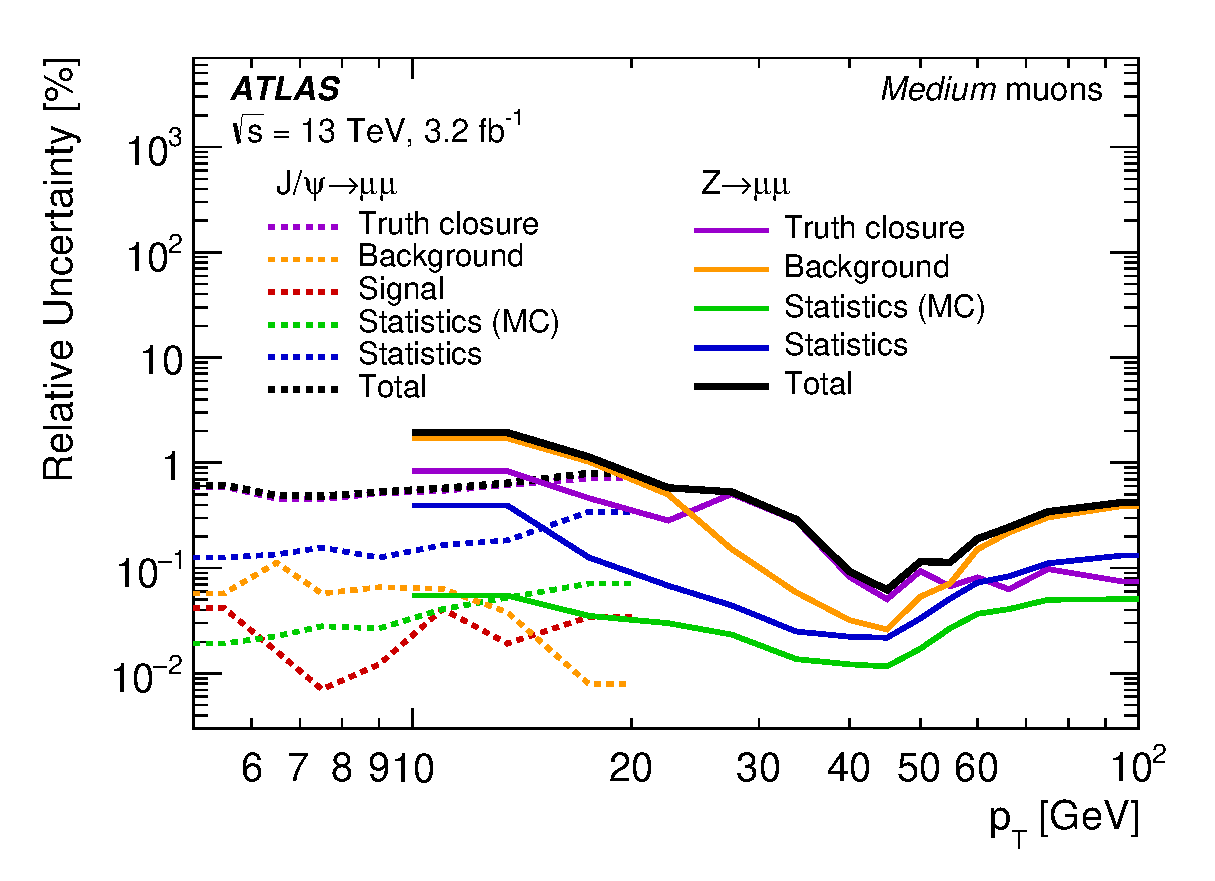
\includegraphics[width=0.8\linewidth]{event_reconstruction/dimuon_efficiency_scale_factor_uncert.eps}
 \caption[Total uncertainty in the efficiency scale factor for Medium muons as a function of $p_{T}$ as obtained from $Z\to\mu\mu$ and $J/\Psi \to \mu\mu$ decays.]{%
  Total uncertainty in the efficiency scale factor for Medium muons as a function of $p_{T}$ as obtained from $Z\to\mu\mu$ (solid lines) and $J/\Psi \to \mu\mu$ (dashed lines) decays.
  The combined uncertainty is the sum in quadrature of the individual contributions~\cite{PERF-2015-10}.}
 \label{fig:dimuon_efficiency_scale_factor_uncert}
\end{figure}

\section{Jets}\label{section:jets}

As particles that carry \gls{QCD} color charge do not exist by themselves in isolation, but form with other colored particles to form colorless composite particles known as ``hadrons,'' it is not possible to directly observe quarks or gluons in ATLAS.
Instead, this process of hadronization, and subsequent decays and rehadronization, creates a shower of both charged and neutral particles that hit the detector, creating charged tracks and energy deposits.
These hadronic showers are stochastic, and there is no way to give a full descriptive definition of them, though there is very impressive recent work on operational definitions~\cite{Metodiev:2018ftz,Komiske:2018vkc,Larkoski:2019nwj}.
Instead, clustering algorithms are used to create collections of tracks and energy deposits, known as ``jets'', based off of the criteria of interest in the algorithm.
In a similar manner to how QCD's depth and richness as a theory requires proper treatment outside the scope of this thesis, jet physics is complex and deep enough to rightly be its own intense physics program at the LHC.
This section will only attempt to give an executive summary of the jet physics and techniques that is pertinent to my thesis analysis --- however for an exceedingly thorough overview see~\cite{Nachman:2016qyc}.

Of the jet clustering algorithms that are common in high energy physics~\cite{Salam:2009jx,Salam:2007xv} the most widely used are the $k_{t}$, Cambridge/Aachen, and anti-$k_{t}$ algorithms~\cite{Cacciari:2008gp,Soyez:2008pq}.
These algorithms are all similar in their approaches with variations on the features they emphasize.
The approach is to iteratively apply the following for all objects in the considered RoI:
\begin{enumerate}
 \item Compute the pairwise distance $d_{ij}$ between objects $i$ and $j$ where
       \[
        d_{ij} = \textrm{min}\left(k_{ti}^{2p}, k_{tj}^{2p}\right) \frac{\Delta_{ij}^{2}}{R^{2}}
       \]
       and $\Delta_{ij}^{2} = \left(y_{i} - y_{j}\right)^{2} + \left(\phi_{i} - \phi_{j}\right)^{2}$ for transverse momentum $k_{t}$, rapidity $y$, and azimuthal angle $\phi$, and parameters of choice $R$, which governs the size of the jet (though it is not a hard cutoff limit), and $p$, which governs the relative power of the energy versus geometrical $\left(\Delta_{ij}\right)$ scales~\cite{Cacciari:2008gp}.
 \item Compute the distance $d_{iB}$ between the object $i$ and the beamline $B$ where $d_{iB} = k_{ti}^{2p}$.
 \item Determine the smallest distance out of the set of distances $d_{ij}$ and $d_{iB}$, $d_{\mathrm{min}} \in \left\{\left\{d_{ij}\right\},\left\{d_{iB}\right\}\right\}$.
 \item If the minimum distance is between the object $i$ and the beamline, $d_{\mathrm{min}} \in \left\{d_{iB}\right\}$, label this object a jet and remove it.
 \item If the minimum distance is between object $i$ and $j$, $d_{\mathrm{min}} \in \left\{d_{ij}\right\}$, group these two objects into a new object $k$ which is added to the object collection, and remove objects $i$ and $j$.
\end{enumerate}
The above is repeated until there are no more remaining objects, at which point all objects have been assigned to a jet.
It is seen that the choice of free parameter $p$ then defines which algorithm is used, and what information the jet clustering algorithm prioritizes.
The choice of $p=1$ corresponds to the $k_{t}$ algorithm~\cite{Catani:1993hr}, which is seen to cluster softer --- less energetic --- objects together into progressively harder --- more energetic --- objects, as seen in \Cref{fig:jet_algorithms_kt}.
Working under the assumption that generally the hardest objects will be towards the center of the shower of particles, this can be seen as an ``outside-in'' clustering which will result in irregularly shaped (probably not very cone-like) jets.
Choosing $p=0$ corresponds to the Cambridge/Aachen jet algorithm~\cite{Dokshitzer:1997in}, which reduces the distance $d_{ij}$ to only include the angular information, $\Delta_{ij}$.
This means that softer splittings of the shower will be clustered into harder branches, which will again produce irregular shaped jets, as seen in \Cref{fig:jet_algorithms_Cambridge_Aachen}.
Choosing $p=-1$ corresponds to the anti-$k_{t}$ algorithm~\cite{Cacciari:2008gp}, where the hardest objects are clustered together first and then subsequently softer objects are added.
The anti-$k_{t}$ algorithm produces relatively regular cone shaped jets that are focused around a hard core, as seen in \Cref{fig:jet_algorithms_anti_kt}.
A typical choice of jet algorithm in ATLAS is the anti-$k_{t}$ algorithm with size parameter of $R=0.4$.

\begin{figure}[htbp]
 \centering
 \begin{subfigure}[t]{0.315\textwidth}
  \centering
  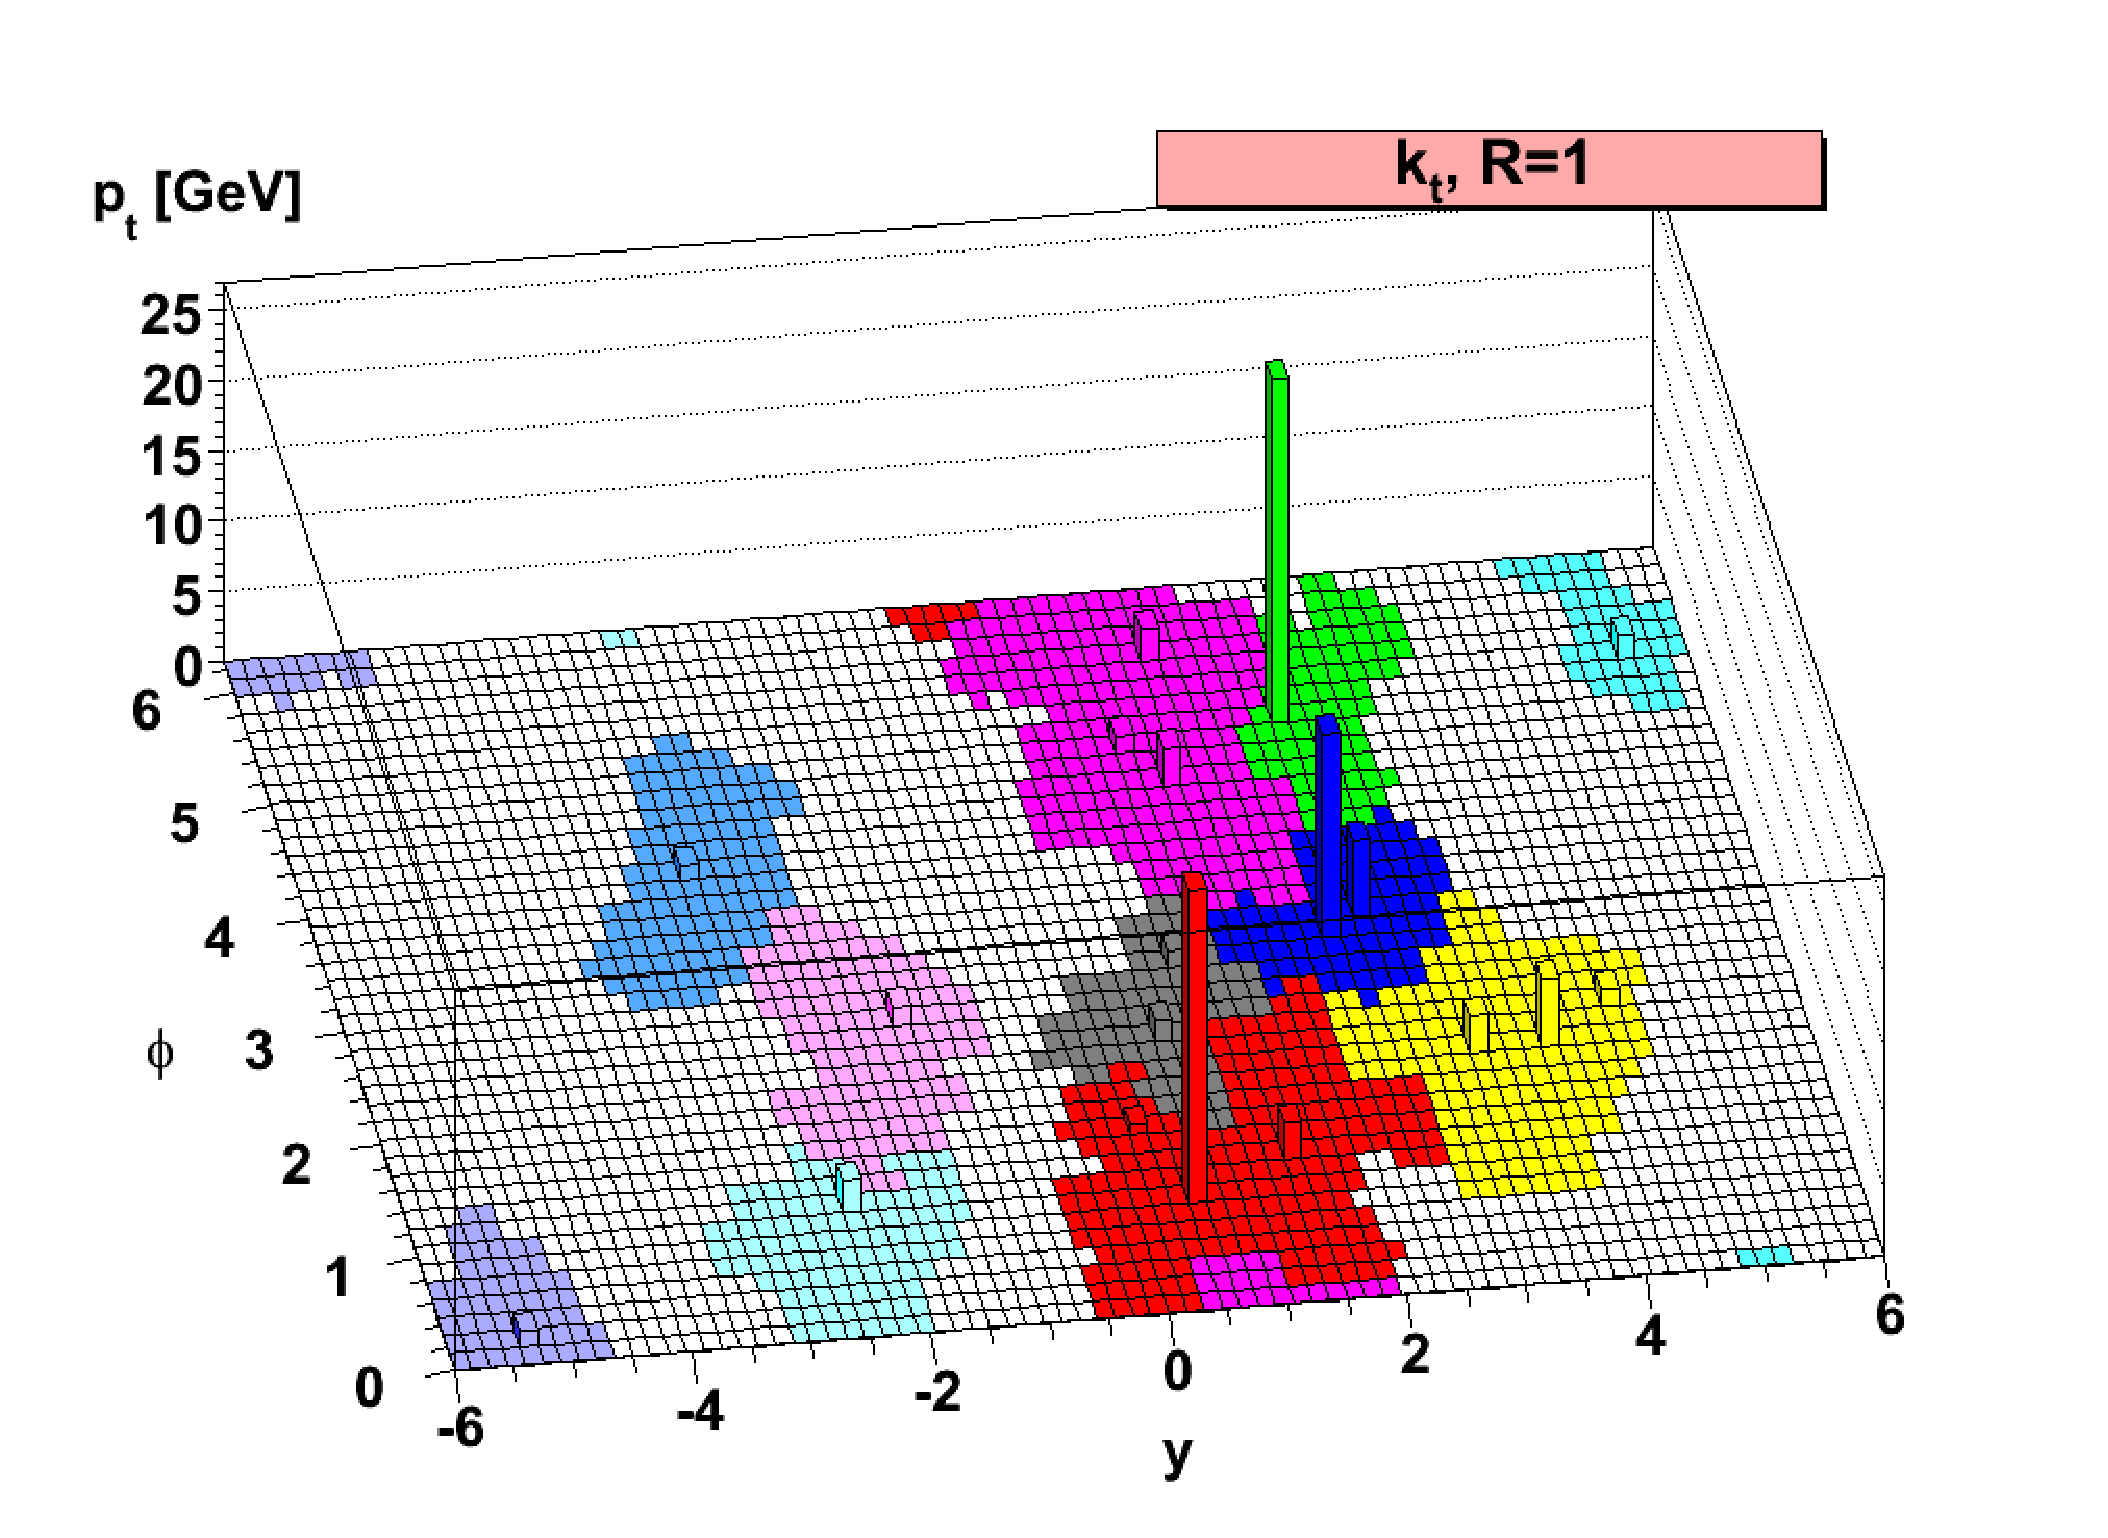
\includegraphics[width=\textwidth]{event_reconstruction/kt.eps}
  \caption[The sample parton-level event clustered with the $k_{t}$ jet algorithm.]{%
   The sample parton-level event clustered with the $k_{t}$ jet algorithm.}
  \label{fig:jet_algorithms_kt}
 \end{subfigure}%
 \quad
 \begin{subfigure}[t]{0.315\textwidth}
  \centering
  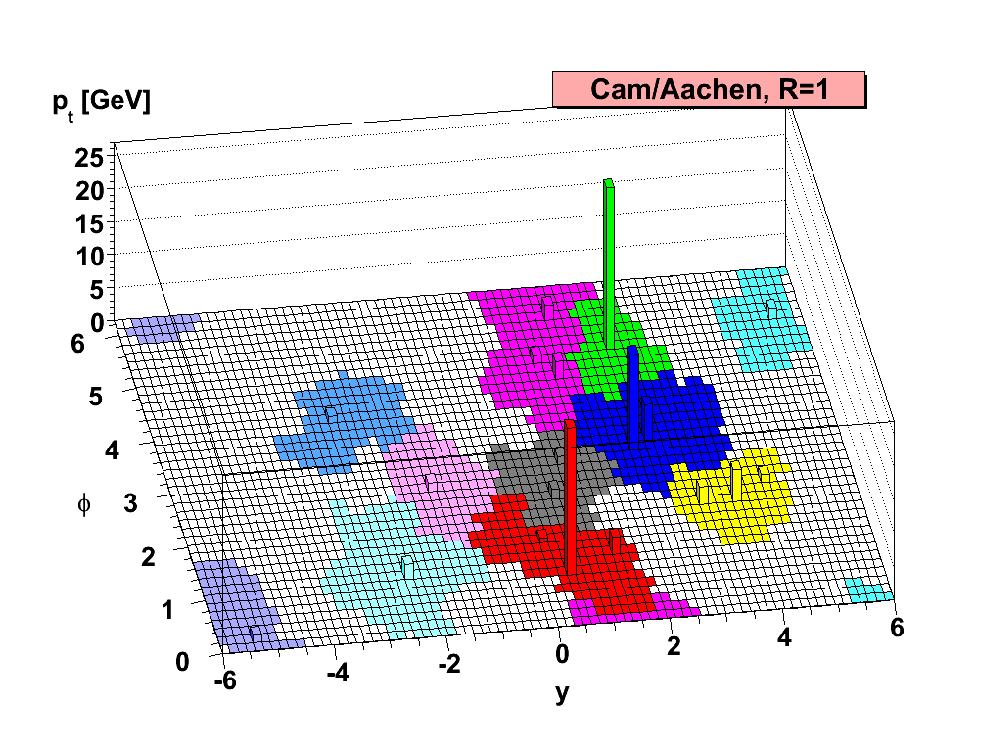
\includegraphics[width=\textwidth]{event_reconstruction/Cambridge_Aachen.eps}
  \caption[The sample parton-level event clustered with the Cambridge/Aachen jet algorithm.]{%
   The sample parton-level event clustered with the Cambridge/Aachen jet algorithm.}
  \label{fig:jet_algorithms_Cambridge_Aachen}
 \end{subfigure}%
 \quad
 \begin{subfigure}[t]{0.315\textwidth}
  \centering
  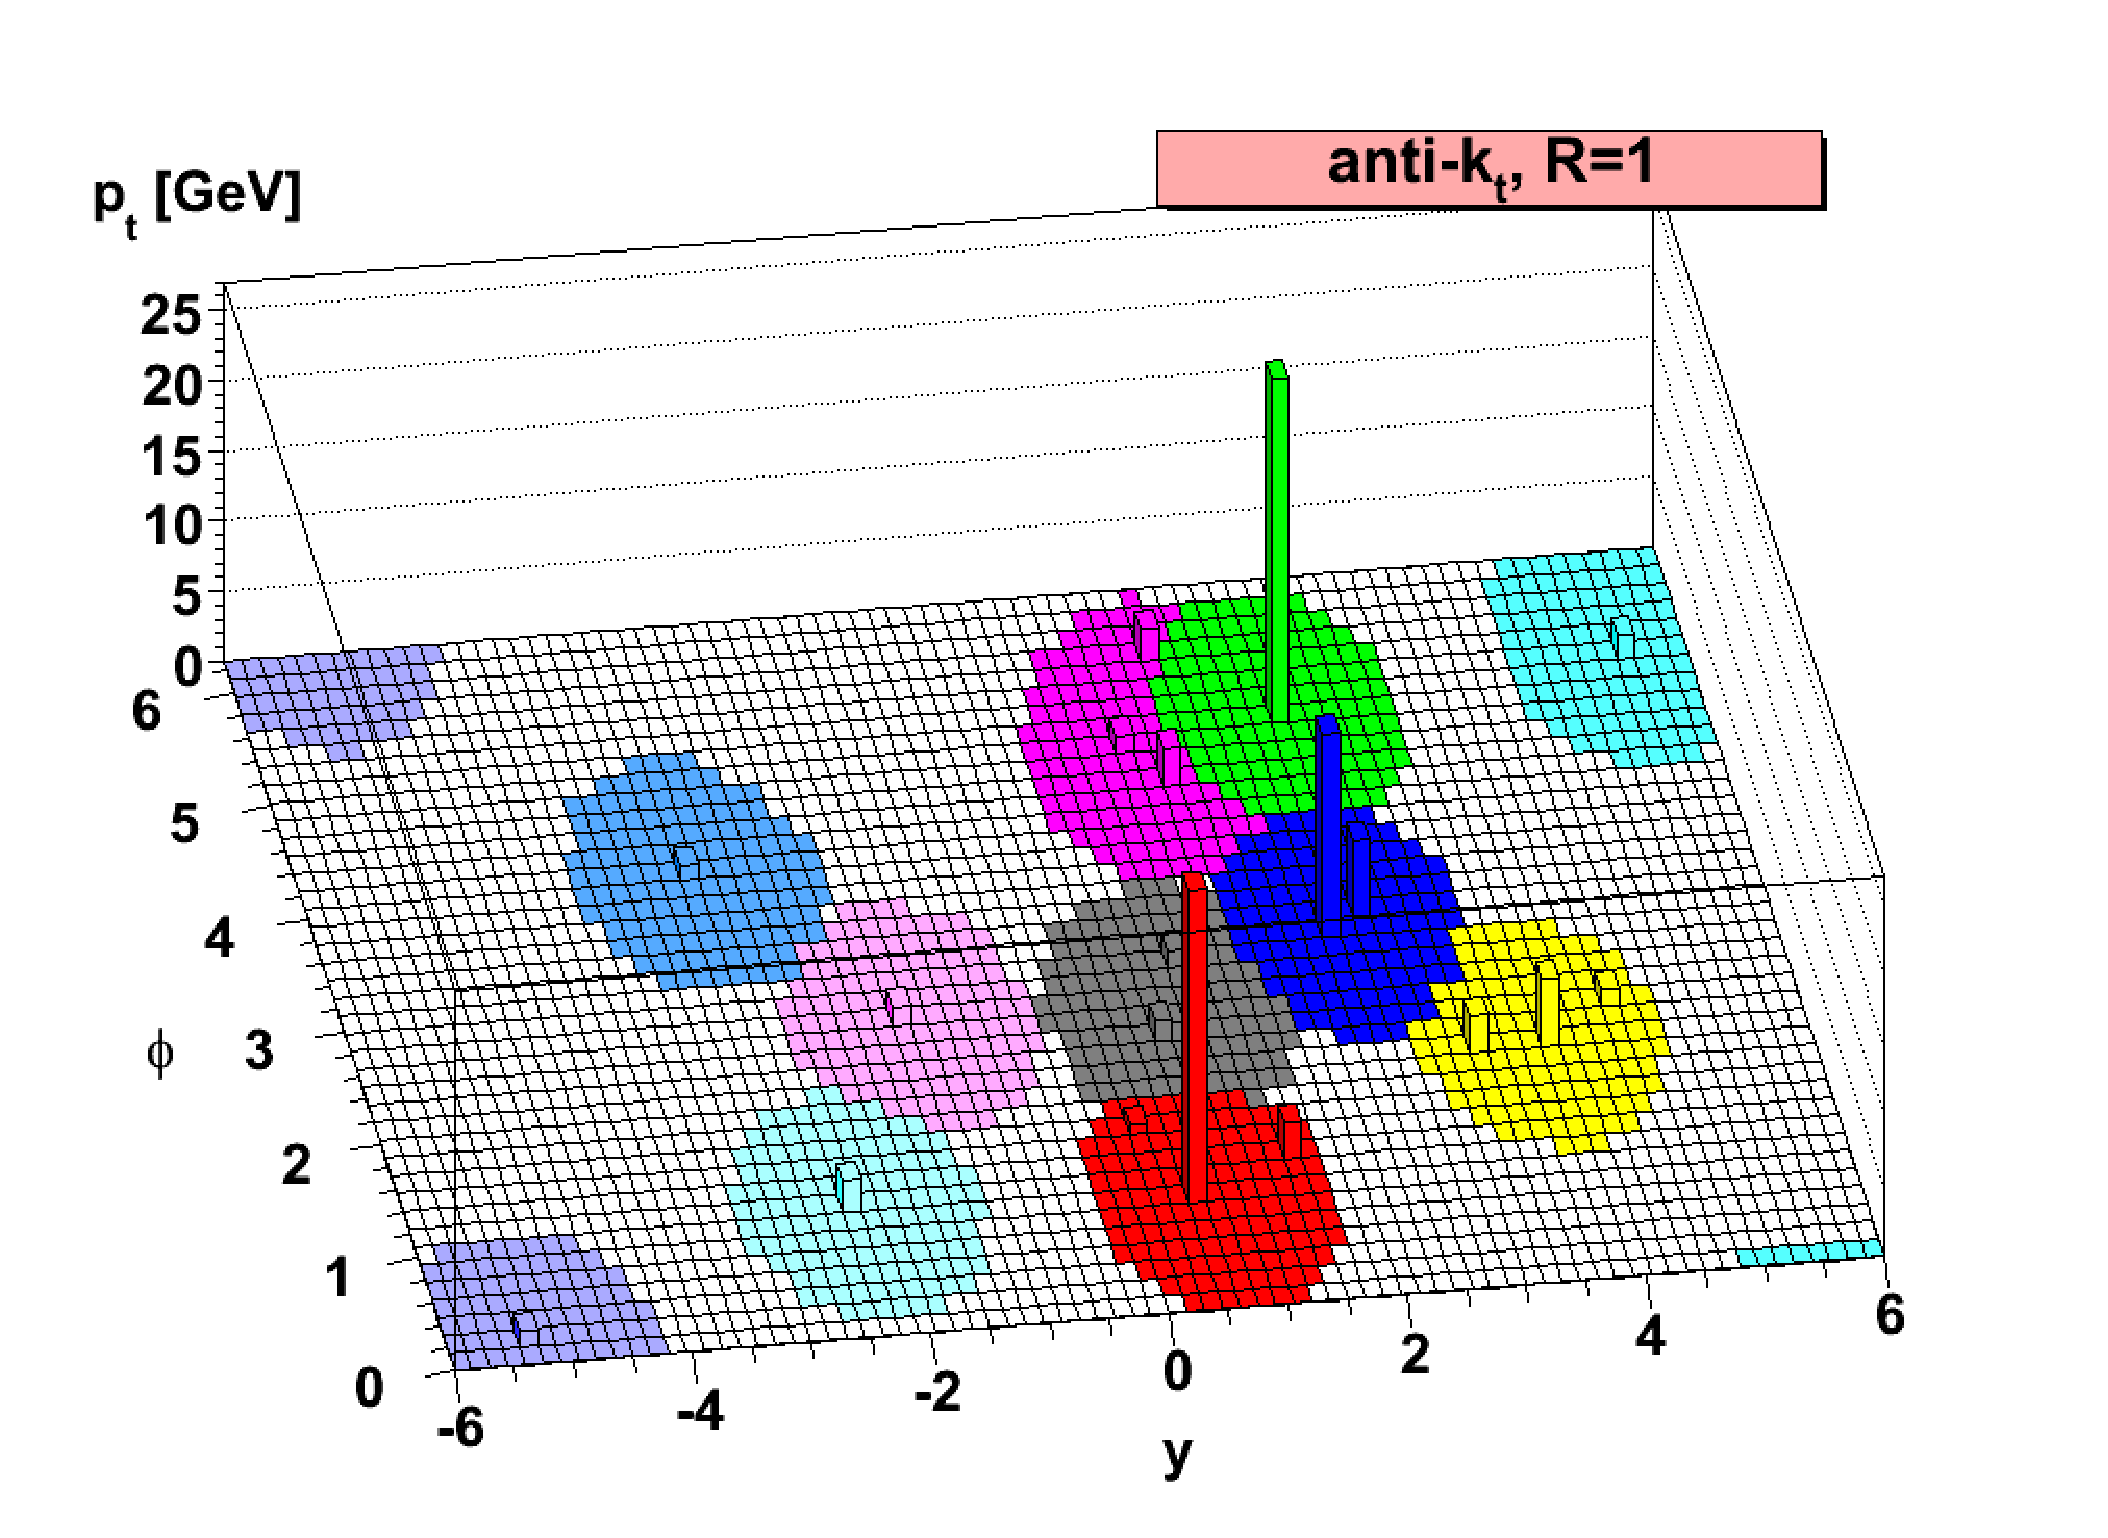
\includegraphics[width=\textwidth]{event_reconstruction/anti_kt.eps}
  \caption[The sample parton-level event clustered with the anti-$k_{t}$ jet algorithm.]{%
   The sample parton-level event clustered with the anti-$k_{t}$ jet algorithm.}
  \label{fig:jet_algorithms_anti_kt}
 \end{subfigure}%
 \caption[A sample parton-level event, together with many random soft ``ghosts'', clustered with three different jet algorithms, illustrating the ``active'' catchment areas of the resulting hard jets.]{%
  A sample parton-level event (generated with Herwig), together with many random soft ``ghosts'', clustered with the $k_{t}$, Cambridge/Aachen, and anti-$k_{t}$ jet algorithms, illustrating the ``active'' catchment areas of the resulting hard jets.
  For $k_{t}$ and Cambridge/Aachen the detailed shapes are in part determined by the specific set of ghosts used, and change when the ghosts are modified~\cite{Cacciari:2008gp}.}
 \label{fig:jet_algorithms}
\end{figure}


\subsection{Large Radius Jets}\label{subsection:largeR_jets}

For analyses that are dealing with very high momentum resonances, the resulting decay products can become highly collimated and be reconstructed as a single jet with a large radius parameter, $R$, (a ``\largeR{}'' jet) typically set to $R=1.0$~\cite{JETM-2018-02,SUSY-2016-13}.
For my thesis analysis \largeR{} jets were used, where the \largeR{} jets were reconstructed from topological clusters in the calorimeters using the anti-$k_{t}$ algorithm with radius parameter of $R=1.0$ and were trimmed~\cite{Krohn:2009th} to improve mass resolution and reduce dependence on pile-up.
The trimming is done by reclustering the \largeR{} jet constituents using the $k_{t}$ algorithm with a radius parameter of $R=0.2$ into subjets, and then removing any subjet that has $p_{T}$ less than $5\%$ of the \largeR{} parent jet's energy.

\subsection{Variable Radius Track Jets}\label{subsection:VR_jets}

In recent years there have been dedicated efforts to improve jet algorithm techniques, especially in the high momentum regime.
As part of these efforts, variable radius (VR) jets~\cite{Krohn:2009zg,ATL-PHYS-PUB-2017-010} were introduced where the radius parameter, $R$, decreases as a function of the jet $p_{T}$,
\[
 R_{\mathrm{eff}} \left(p_{T}\right)= \frac{\rho}{p_{T}},
\]
where the dimensionful constant $\rho$ determines how fast the effective jet size decreases with the transverse momentum of the jet.
The choice of $\rho$ should be proportional to the mass of the resonance, and so should correctly reproduce the size of jets as long as $\rho \lesssim 2 p_{T}$.
Additional parameters $R_{\mathrm{min}}$ and $R_{\mathrm{max}}$ are used to to impose
lower and upper cut-offs on the jet size,
\[
 R_{\mathrm{eff}} \left(p_{T}\right)= \mathrm{max}\left[\mathrm{min}\left(\frac{\rho}{p_{T}},R_{\mathrm{max}}\right),R_{\mathrm{min}}\right]\,.
\]
For my thesis analysis variable radius track jets~\cite{Zenz:2010hfa} were used with $\rho=30~\GeV$, $R_{\mathrm{min}}=0.02$, and $R_{\mathrm{max}}=0.4$, which in simulation gives the highest truth sujbet double $b$-labelling efficiency for high $p_{T}$ Higgs bosons~\cite{ATL-PHYS-PUB-2017-010}, as seen in \Cref{fig:VR_jets_parameters}.
It is seen from \Cref{fig:VR_jets_lead_subjet}, \Cref{fig:VR_jets_sublead_subjet}, and \Cref{fig:Higgs_VR_DeltaR} that VR track jets are able to describe the topology of $\Hbb$ events across high $p_{T}$ spectrum much more accurately than fixed radius $R=0.2$ track jets, making their use an excellent choice for the analysis.

\begin{figure}[htbp]
 \centering
 \begin{subfigure}[t]{0.48\textwidth}
  \centering
  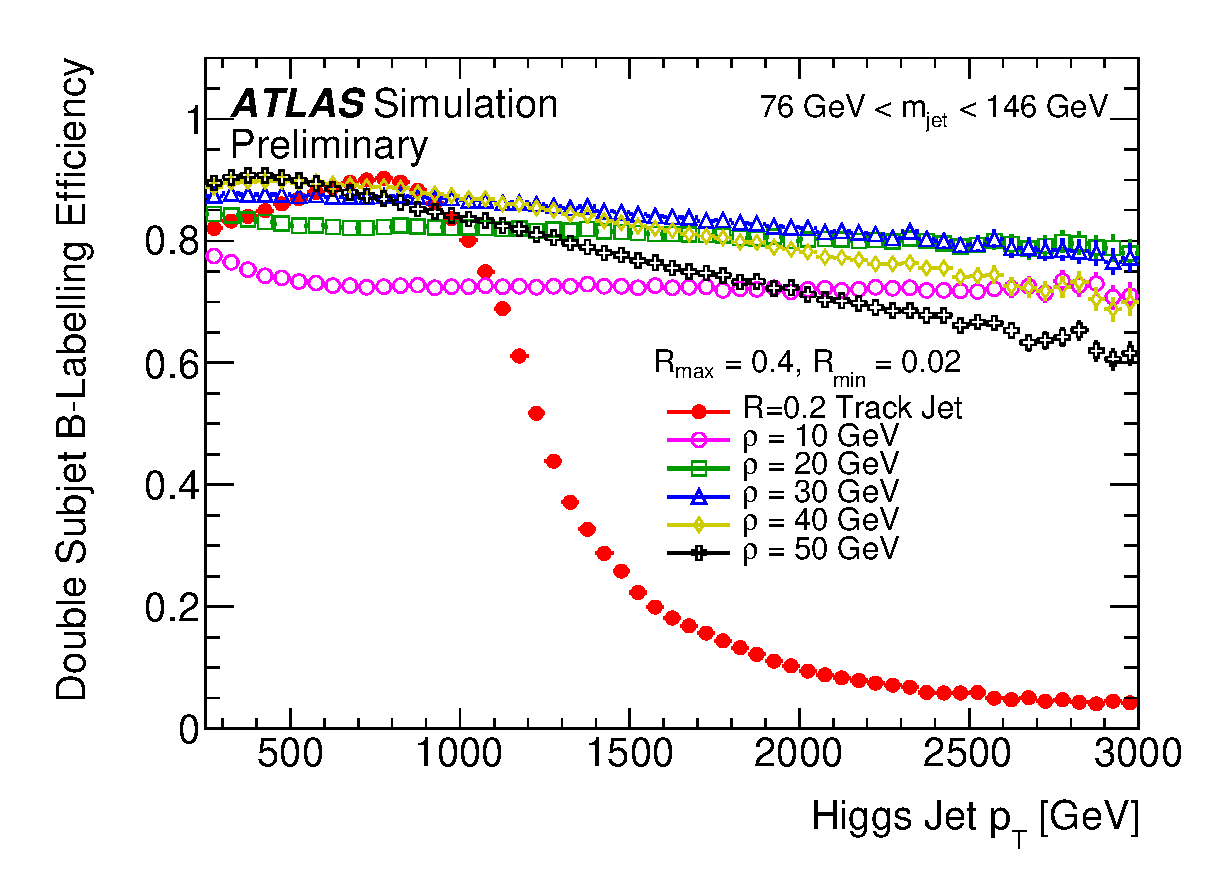
\includegraphics[width=\textwidth]{event_reconstruction/VR_jets_rho_values.eps}
  \caption[The efficiency for VR track jets with ${R_{\mathrm{min}}=0.02}$ and ${R_{\mathrm{max}} = 0.4}$ for several $\rho$ values.]{%
   The efficiency for VR track jets with ${R_{\mathrm{min}}=0.02}$ and ${R_{\mathrm{max}} = 0.4}$ for several $\rho$ values.}
  \label{fig:VR_jets_rho_values}
 \end{subfigure}%
 \quad
 \begin{subfigure}[t]{0.48\textwidth}
  \centering
  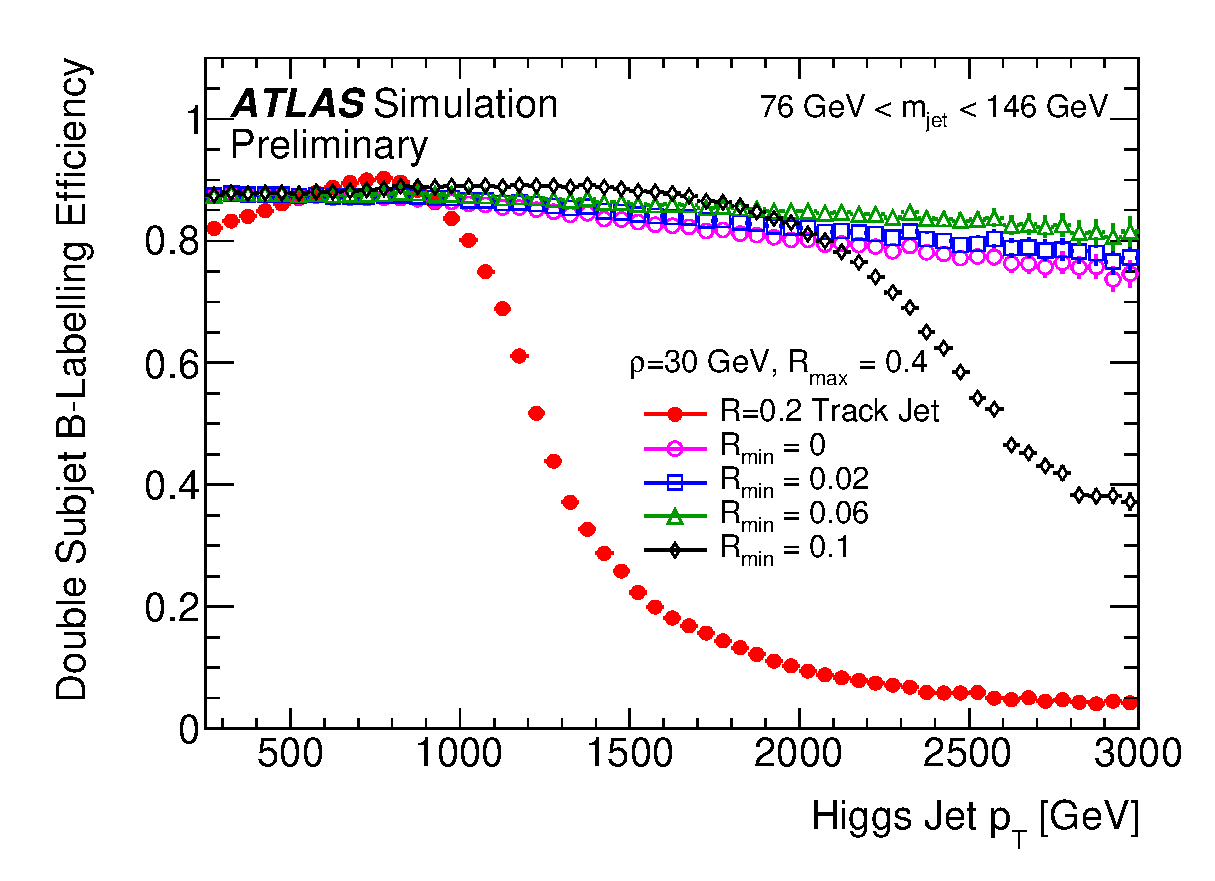
\includegraphics[width=\textwidth]{event_reconstruction/VR_jets_Rmin.eps}
  \caption[The efficiency for VR track jets with ${\rho=30~\GeV}$ and ${R_{\mathrm{max}} = 0.4}$ for different values of $R_{\mathrm{min}}$.]{%
   The efficiency for VR track jets with ${\rho=30~\GeV}$ and ${R_{\mathrm{max}} = 0.4}$ for different values of $R_{\mathrm{min}}$.}
  \label{fig:VR_jets_Rmin}
 \end{subfigure}%

 \begin{subfigure}[t]{0.48\textwidth}
  \centering
  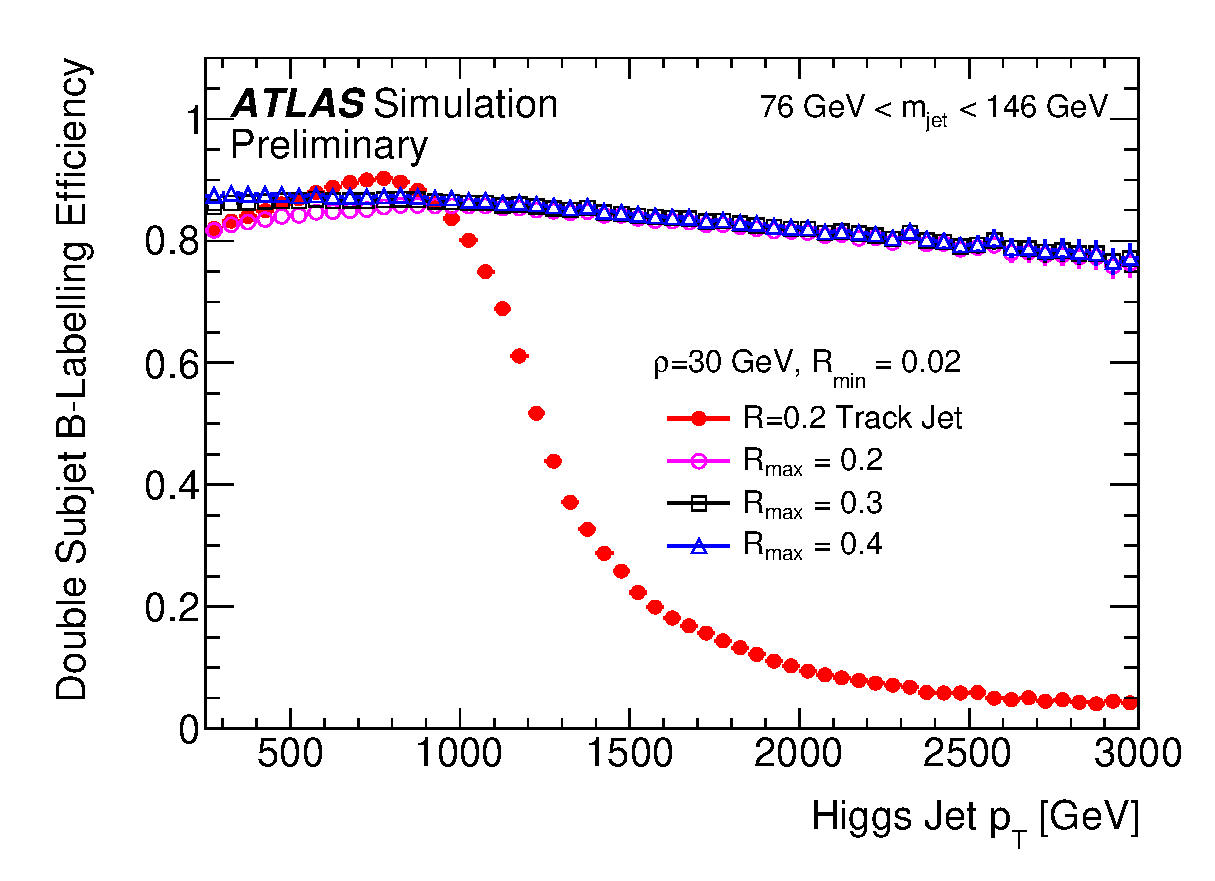
\includegraphics[width=\textwidth]{event_reconstruction/VR_jets_Rmax.eps}
  \caption[The efficiency for VR track jets with ${\rho=30~\GeV}$ and ${R_{\mathrm{min}} = 0.02}$ for varying values of $R_{\mathrm{max}}$.]{%
   The efficiency for VR track jets with ${\rho=30~\GeV}$ and ${R_{\mathrm{min}} = 0.02}$ for varying values of $R_{\mathrm{max}}$.}
  \label{fig:VR_jets_Rmax}
 \end{subfigure}%
 \caption[Efficiency of subjet double $b$-labelling at the truth level of a Higgs jet as a function of the Higgs jet $p_{T}$.]{%
  Efficiency of subjet double $b$-labelling at the truth level of a Higgs jet as a function of the Higgs jet $p_{T}$.
  The efficiency for $R=0.2$ track jets is also included in all of the plots.
  The uncertainty bars include statistical uncertainties only~\cite{ATL-PHYS-PUB-2017-010}.}
 \label{fig:VR_jets_parameters}
\end{figure}

\begin{figure}[htbp]
 \centering
 \begin{subfigure}[t]{0.48\textwidth}
  \centering
  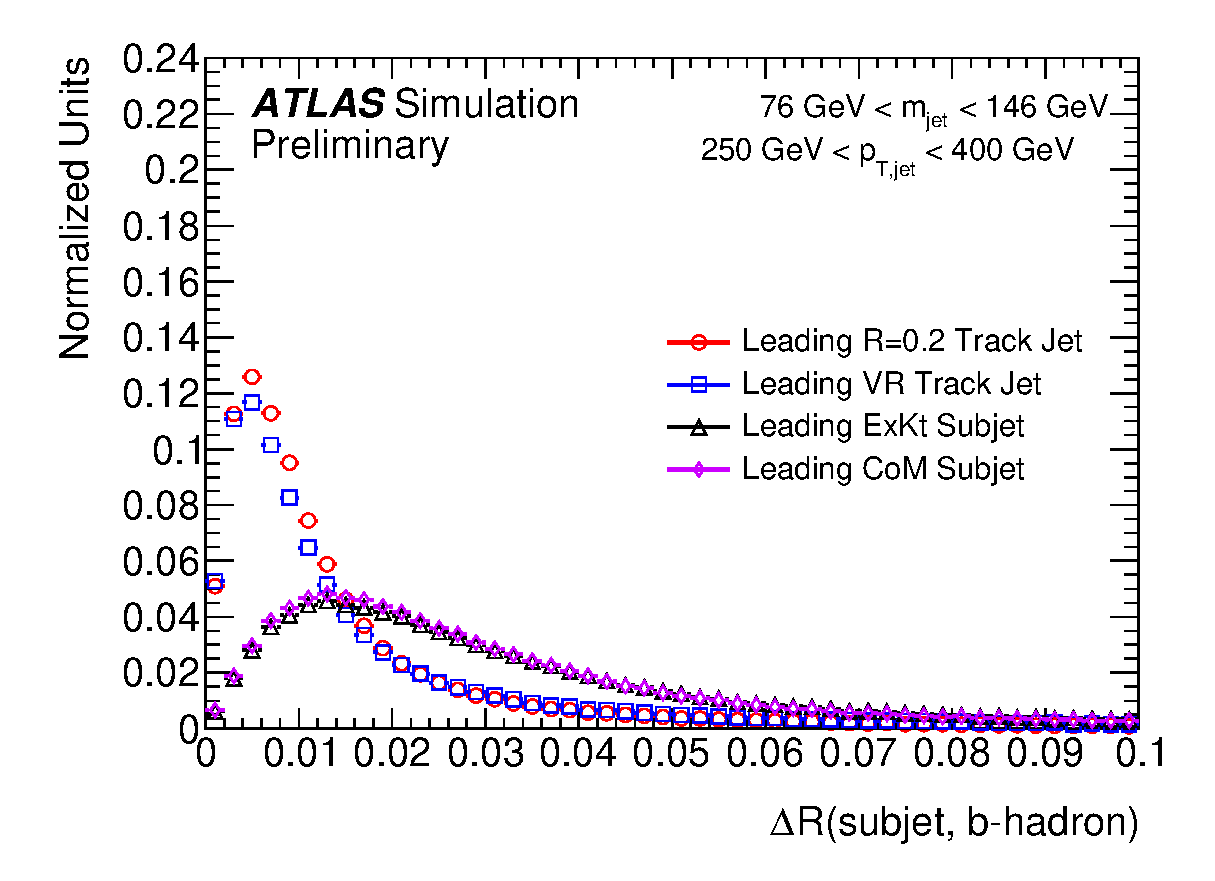
\includegraphics[width=\textwidth]{event_reconstruction/VR_jets_lead_subjet_low.eps}
  \caption[Distributions of the $\Delta R$ between leading subjets and matched truth $b$-hadrons for Higgs with low jet $p_{T}$ of ${250~\GeV < p_{T} < 400~\GeV}$.]{%
   Distributions of the $\Delta R$ between leading subjets and matched truth $b$-hadrons for Higgs with low jet $p_{T}$ of ${250~\GeV < p_{T} < 400~\GeV}$.}
  \label{fig:VR_jets_lead_subjet_low}
 \end{subfigure}%
 \quad
 \begin{subfigure}[t]{0.48\textwidth}
  \centering
  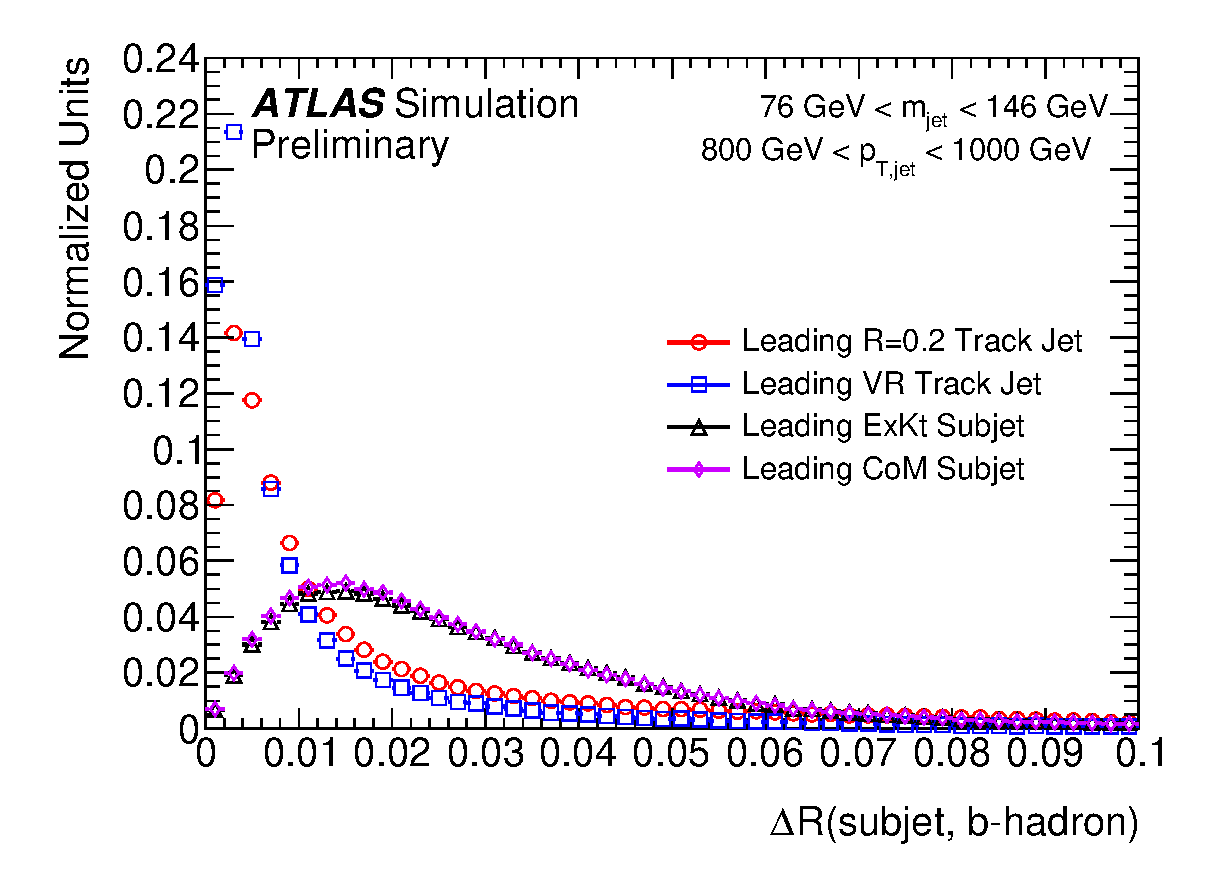
\includegraphics[width=\textwidth]{event_reconstruction/VR_jets_lead_subjet_high.eps}
  \caption[Distributions of the $\Delta R$ between leading subjets and matched truth $b$-hadrons for Higgs with high jet $p_{T}$ of ${800~\GeV < p_{T} < 1000~\GeV}$.]{%
   Distributions of the $\Delta R$ between leading subjets and matched truth $b$-hadrons for Higgs with high jet $p_{T}$ of ${800~\GeV < p_{T} < 1000~\GeV}$.}
  \label{fig:VR_jets_lead_subjet_high}
 \end{subfigure}%
 \caption[Distributions of the $\Delta R$ between leading subjets and matched truth $b$-hadrons for two different Higgs jet $p_{T}$ bins.]{%
  Distributions of the $\Delta R$ between leading subjets and matched truth $b$-hadrons for low Higgs jet $p_{T}$ of ${250~\GeV < p_{T} < 400~\GeV}$ and high Higgs jet $p_{T}$ of ${800~\GeV < p_{T} < 1000~\GeV}$.
  The uncertainty bars include statistical uncertainties only.
  All algorithms have been normalized to an area corresponding to the fraction of signal jets which contain a leading subjet~\cite{ATL-PHYS-PUB-2017-010}.}
 \label{fig:VR_jets_lead_subjet}
\end{figure}

\begin{figure}[htbp]
 \centering
 \begin{subfigure}[t]{0.48\textwidth}
  \centering
  \includegraphics[width=\textwidth]{event_reconstruction/VR_jets_sublead_subjet_low.eps}
  \caption[Distributions of the $\Delta R$ between subleading subjets and matched truth $b$-hadrons for Higgs with low jet $p_{T}$ of ${250~\GeV < p_{T} < 400~\GeV}$.]{%
   Distributions of the $\Delta R$ between subleading subjets and matched truth $b$-hadrons for Higgs with low jet $p_{T}$ of ${250~\GeV < p_{T} < 400~\GeV}$.}
  \label{fig:VR_jets_sublead_subjet_low}
 \end{subfigure}%
 \quad
 \begin{subfigure}[t]{0.48\textwidth}
  \centering
  \includegraphics[width=\textwidth]{event_reconstruction/VR_jets_sublead_subjet_high.eps}
  \caption[Distributions of the $\Delta R$ between subleading subjets and matched truth $b$-hadrons for Higgs with high jet $p_{T}$ of ${800~\GeV < p_{T} < 1000~\GeV}$.]{%
   Distributions of the $\Delta R$ between subleading subjets and matched truth $b$-hadrons for Higgs with high jet $p_{T}$ of ${800~\GeV < p_{T} < 1000~\GeV}$.}
  \label{fig:VR_jets_sublead_subjet_high}
 \end{subfigure}%
 \caption[Distributions of the $\Delta R$ between subleading subjets and matched truth $b$-hadrons for two different Higgs jet $p_{T}$ bins.]{%
  Distributions of the $\Delta R$ between subleading subjets and matched truth $b$-hadrons for low Higgs jet $p_{T}$ of ${250~\GeV < p_{T} < 400~\GeV}$ and high Higgs jet $p_{T}$ of ${800~\GeV < p_{T} < 1000~\GeV}$.
  The uncertainty bars include statistical uncertainties only.
  All algorithms have been normalized to an area corresponding to the fraction of signal jets which contain a leading subjet~\cite{ATL-PHYS-PUB-2017-010}.}
 \label{fig:VR_jets_sublead_subjet}
\end{figure}

\begin{figure}[htbp]
 \centering
 \includegraphics[width=0.8\linewidth]{event_reconstruction/Higgs_VR_DeltaR.eps}
 \caption[The $\Delta R$ between the two leading truth $b$-hadrons or subjets associated to Higgs jets as a function of Higgs jet $p_{T}$.]{%
  The $\Delta R$ between the two leading truth $b$-hadrons or subjets associated to Higgs jets as a function of Higgs jet $p_{T}$~\cite{Salzburger:HammersAndNails}.}
 \label{fig:Higgs_VR_DeltaR}
\end{figure}

\section{Flavor Tagging}\label{section:flavor_tagging}

Flavor tagging of jets is the process of determining a ``flavor'' label --- light, charm $(c)$, or bottom $(b)$ --- to characterize the type of hadrons in the hadronic shower that resulted in the jet.
Flavor tagging is vital in precision measurements in the top quark sector%
\footnote{Noting that the top quark has a branching fraction of $\mathcal{B}\left(t \to W b\right) = 0.96_{-0.066}^{+0.068}\left(\mathrm{stat.}\right)_{-0.052}^{+0.064}\left(\mathrm{syst.}\right)$~\cite{Abazov:2010tm,PhysRevD.98.030001}.}%
, in the search for the Higgs boson as well as new phenomena decaying to $b\bar{b}$ states, and, in particular importance to this thesis analysis, the suppression of background processes that contain predominantly light-flavor jets~\cite{PERF-2012-04}.
Of particular great interest in flavor tagging is $b$-tagging (labeling of jets containing $B$ hadrons --- $b$-jets), as $B$ hadrons are often produced in decays of heavy resonances that could be indicative of interesting new physics.
$B$ hadrons have a number of unique properties that distinguish them, as seen in \Cref{fig:b_jet}.
Notable among them is their long lifetime, discussed in \Cref{appendix:B_hadron_lifetimes}, of approximately $1.5~\mathrm{ps}$ which gives a characteristic length scale of $c\tau \sim 0.45~\mathrm{mm}$.
This is a significant enough flight distance of the $B$ meson before it decays, that this subsequent hadron shower and jet is viewed as having a secondary vertex (SV) displaced from the original jet vertex.
This secondary vertex is detectable as the vertex resolution in ATLAS for $50$ associated tracks is approximately $20~\mu\mathrm{m}$ in $r$-$\phi$ by $30~\mu\mathrm{m}$ in $z$~\cite{Choi:2271033,ATL-PHYS-PUB-2015-026}.
$B$ mesons also have a mass of approximately $5~\GeV$.
Collectively, these properties can be exploited by $b$-tagging algorithms to discriminate $b$-jets from light or charm jets~\cite{ATL-PHYS-PUB-2015-022,ATL-PHYS-PUB-2016-012,ATL-PHYS-PUB-2017-013,PERF-2016-05}.

\begin{figure}[htbp]
 \centering
 \centering
 \includegraphics[width=0.6\textwidth]{event_reconstruction/b_jet.pdf}
 \caption[Cartoon of a typical $b$-jet.]{%
  Cartoon of a typical $b$-jet containing a $b$-hadron decay vertex (\textcolor{track_blue}{blue}~\tikzdot{track_blue}) displaced from the primary $pp$ vertex (\textcolor{red}{red}~\tikzdot{red}), and a $c$-hadron decay vertex (\textcolor{orange}{orange}~\tikzdot{orange}) further displaced and often close to the $b$-hadron flight axis.
  Tracks from secondary (\textcolor{track_blue}{blue}) and tertiary (\textcolor{orange}{orange}) vertices have large impact parameters (\textcolor{IPgreen}{green}) with respect to the primary $pp$ vertex~\cite{Chisholm:bjet}.}
 \label{fig:b_jet}
\end{figure}

It is seen from \Cref{fig:signed_impact_parameters} that the transverse and longitudinal impact parameters --- respectively, $d_{0}$ and $z_{0}$ --- of $b$-jets tend to be positive, while $c$-jets and light-jets tend to have more impact parameters distributed more symmetrically around $0$.
As a result, these impact parameters can be used as inputs to discriminating algorithms.
For the data taking periods of my thesis analysis the main $b$-tagging algorithm used in ATLAS was the \texttt{MV2c10} Boosted Decision Tree (BDT) based algorithm.%
\footnote{\texttt{MV2c10} is named to reflect that it is a multivariate algorithm with the fraction of $c$-jets in the training sample at roughly $10\%$.
 In reality the $c$-jet fraction is $7\%$ and the light-jet fraction is $93\%$ to give a good balance between light-jet and $c$-jet rejection.}
In addition to the quantities of the jet itself, \texttt{MV2c10} uses the output of other lower level $b$-tagging algorithms as inputs, as seen in \Cref{fig:MV2_inputs}.
These include the likelihood ratio based two-dimensional and three-dimensional impact parameter algorithms, IP2D and IP3D.
The IP2D and IP3D algorithms assume that the track IPs are uncorrelated.
The output of IP3D is shown in \Cref{fig:IP3D_LLR} for the 2017 and 2018 data taking optimization of using a training sample of $50\%$ $t\bar{t}$ and $50\%$ $\Zprime \to q\bar{q}$ for $q\in\left\{\mathrm{light}, c, b\right\}$ to cover a large $p_{T}$ range of jets.
The 2016 optimization used a training sample of $50\%$ $t\bar{t}$ and $50\%$ $\Zprime \to t\bar{t}$.
In the 2017 data taking a Recurrent Neural Network (RNN) impact parameter tagger (RNNIP)~\cite{ATL-PHYS-PUB-2017-003} was added as well, that exploits the correlations between the impact parameters between the tracks, as $b$-jets tend to have multiple highly significant IP tracks, while this is not the case for light flavor jets, as seen in \Cref{fig:RNNIP_track_significance}.
There are additional displaced secondary vertex finding algorithms (SV1), and Kalman filter algorithms (JetFitter) that exploit that roughly $90\%$ of $b$-jets contain a $c$-jet and so follow this decay chain.
Additionally a Soft Muon Tagger is also added which in the 2017 data taking based on
the reconstruction of muons from the semileptonic decay of $b$-hadrons and $c$-hadrons.
The \texttt{MV2c10} BDT combines all these inputs and then gives a discriminant score indicative of how $b$-jet-like or how un-$b$-jet-like the inputs are given its training, as seen in \Cref{fig:MV2c10_BDT}.
The \texttt{MV2c10} BDT is trained using $t\bar{t}$ for the 2016 optimization, and a hybrid sample of $t\bar{t}$ and $\Zprime$ to cover a wide $p_{T}$ spectrum for the 2017 optimization.
The performance of the BDT is calibrated in data using jets that contain a muon, indicative of the semileptonic decay of a $b$-hadron, and a correction scale factor is derived.

\begin{figure}[htbp]
 \centering
 \centering
 \includegraphics[width=\textwidth]{event_reconstruction/MV2_inputs.pdf}
 \caption[Inputs to the high level $b$-tagging algorithm \texttt{MV2c10} for data taking in 2017 and 2018.]{%
  Inputs to the high level $b$-tagging algorithm \texttt{MV2c10} for data taking in 2017 and 2018~\cite{Feickert:ML4Jets2018}.}
 \label{fig:MV2_inputs}
\end{figure}

\begin{figure}[htbp]
 \centering
 \begin{subfigure}[t]{0.48\textwidth}
  \centering
  \includegraphics[width=\textwidth]{event_reconstruction/IP3D_d0_2016.eps}
  \caption[Transverse impact parameter significance values for the 2016 configuration of the IP3D algorithm.]{%
   Data-MC comparisons of the transverse impact parameter significance values for the 2016 configuration of the IP3D algorithm.}
  \label{fig:IP3D_d0_2016}
 \end{subfigure}%
 \quad
 \begin{subfigure}[t]{0.48\textwidth}
  \centering
  \includegraphics[width=\textwidth]{event_reconstruction/IP3D_d0_2017.eps}
  \caption[Transverse impact parameter significance values for the 2017 configuration of the IP3D algorithm.]{%
   Data-MC comparisons of the transverse impact parameter significance values for the 2017 configuration of the IP3D algorithm.}
  \label{fig:IP3D_d0_2017}
 \end{subfigure}%

 \begin{subfigure}[t]{0.48\textwidth}
  \centering
  \includegraphics[width=\textwidth]{event_reconstruction/IP3D_z0_2016.eps}
  \caption[Longitudinal impact parameter significance values for the 2016 configuration of the IP3D algorithm.]{%
   Data-MC comparisons of the longitudinal impact parameter significance values for the 2016 configuration of the IP3D algorithm.}
  \label{fig:IP3D_z0_2016}
 \end{subfigure}%
 \quad
 \begin{subfigure}[t]{0.48\textwidth}
  \centering
  \includegraphics[width=\textwidth]{event_reconstruction/IP3D_z0_2017.eps}
  \caption[Longitudinal impact parameter significance values for the 2017 configuration of the IP3D algorithm.]{%
   Data-MC comparisons of the longitudinal impact parameter significance values for the 2017 configuration of the IP3D algorithm.}
  \label{fig:IP3D_z0_2017}
 \end{subfigure}%
 \caption[Data-Monte Carlo comparisons of the transverse and longitudinal impact parameter significance values for IP3D selected tracks in the leading jet of the $Z\to\mu\mu + \textrm{jets}$ dominated sample.]{%
  Data-Monte Carlo comparisons of the transverse and longitudinal impact parameter significance values for IP3D selected tracks in the leading jet of a $Z\to\mu\mu + \textrm{jets}$ dominated sample~\cite{ATL-PHYS-PUB-2017-013}.}
 \label{fig:signed_impact_parameters}
\end{figure}

\begin{figure}[htbp]
 \centering
 \begin{subfigure}[t]{0.48\textwidth}
  \centering
  \includegraphics[width=\textwidth]{event_reconstruction/IP3D_LLR_ttbar.eps}
  \caption[Data-Monte Carlo comparison of the IP3D log-likelihood ratio using a $t\bar{t}$-dominated $e\mu$ sample.]{%
   Data-Monte Carlo comparison of the IP3D log-likelihood ratio using a $t\bar{t}$-dominated $e\mu$-dominated sample.}
  \label{fig:IP3D_LLR_ttbar}
 \end{subfigure}%
 \quad
 \begin{subfigure}[t]{0.48\textwidth}
  \centering
  \includegraphics[width=\textwidth]{event_reconstruction/IP3D_LLR_Zjets.eps}
  \caption[Data-Monte Carlo comparison of the IP3D log-likelihood ratio using a $Z\to \mu^{+}\mu^{-}+\textrm{jets}$-dominated sample.]{%
   Data-Monte Carlo comparison of the IP3D log-likelihood ratio using a $Z\to \mu^{+}\mu^{-}+\textrm{jets}$-dominated sample.}
  \label{fig:IP3D_LLR_Zjets}
 \end{subfigure}%
 \caption[Data-Monte Carlo comparison of the log-likelihood ratio used to discriminate the $b$-jet from the light-flavour jet hypotheses in the IP3D $b$-tagging algorithm using different samples.]{%
  Data-Monte Carlo comparison of the log-likelihood ratio used to discriminate the $b$-jet from the light-flavour jet hypotheses in the IP3D $b$-tagging algorithm using a $t\bar{t}$-dominated $e\mu$ sample and a ${Z\to \mu^{+}\mu^{-}+\textrm{jets}}$-dominated sample~\cite{ATL-PHYS-PUB-2017-013}.}
 \label{fig:IP3D_LLR}
\end{figure}

\begin{figure}[htbp]
 \centering
 \begin{subfigure}[t]{0.48\textwidth}
  \centering
  \includegraphics[width=\textwidth]{event_reconstruction/d0_sig_correlations_bjet.pdf}
  \caption[The distribution of the $d_{0}$ significance for the leading $d_{0}$ significance track and subleading $d_{0}$ significance track in $b$-jets jets.]{%
   The distribution of the $d_{0}$ significance for the leading $d_{0}$ significance track and subleading $d_{0}$ significance track in $b$-jets jets.}
  \label{fig:d0_sig_correlations_bjet}
 \end{subfigure}%
 \quad
 \begin{subfigure}[t]{0.48\textwidth}
  \centering
  \includegraphics[width=\textwidth]{event_reconstruction/d0_sig_correlations_lightjet.pdf}
  \caption[The distribution of the $d_{0}$ significance for the leading $d_{0}$ significance track and subleading $d_{0}$ significance track in light jets.]{%
   The distribution of the $d_{0}$ significance for the leading $d_{0}$ significance track and subleading $d_{0}$ significance track in light jets.}
  \label{fig:d0_sig_correlations_lightjet}
 \end{subfigure}%
 \caption[The distribution of the $d_{0}$ significance for the leading $d_{0}$ significance track and subleading $d_{0}$ significance track in $b$-jets and light jets.]{%
  The distribution of the $d_{0}$ significance for the leading $d_{0}$ significance track and subleading $d_{0}$ significance track in $b$-jets and light jets.
  The distributions were produced with 700 thousand $b$-jets and 1 million light jets, and each distribution is normalized to unity~\cite{ATL-PHYS-PUB-2017-003}.}
 \label{fig:RNNIP_track_significance}
\end{figure}

\begin{figure}[htbp]
 \centering
 \begin{subfigure}[t]{0.48\textwidth}
  \centering
  \includegraphics[width=\textwidth]{event_reconstruction/MV2c10_BDT_output.eps}
  \caption[The \texttt{MV2c10} output for $b$-jets, $c$-jets, and light-flavor jets in simulated $t\bar{t}$ events.]{%
   The \texttt{MV2c10} output for $b$-jets (solid line), $c$-jets (dashed line), and light-flavor jets (dotted line) in simulated $t\bar{t}$ events.}
  \label{fig:MV2c10_BDT_output}
 \end{subfigure}%
 \quad
 \begin{subfigure}[t]{0.48\textwidth}
  \centering
  \includegraphics[width=\textwidth]{event_reconstruction/MV2c10_background_rejection.eps}
  \caption[The light-flavor jet and $c$-jet rejection factors as a function of the $b$-jet tagging efficiency of the \texttt{MV2c10} $b$-tagging algorithm.]{%
   The light-flavor jet (dashed line) and $c$-jet rejection factors (solid line) as a function of the $b$-jet tagging efficiency of the \texttt{MV2c10} $b$-tagging algorithm.}
  \label{fig:MV2c10_background_rejection}
 \end{subfigure}%
 \caption[The performance of the \texttt{MV2c10} BDT $b$-tagging algorithm in simulated $t\bar{t}$ events.]{%
  The performance of the \texttt{MV2c10} BDT $b$-tagging algorithm in simulated $t\bar{t}$ events.
  The performance was evaluated on $t\bar{t}$ events simulated using \textsc{Powheg} interfaced to \textsc{Pythia6}~\cite{PERF-2016-05}.}
 \label{fig:MV2c10_BDT}
\end{figure}

\clearpage
\section{Taus}\label{section:taus}

Tau leptons also produced in collisions in ATLAS, however, given their short lifetime they will decay into other SM particles before entering the detector subsystems and are reconstructed as other physics objects.
When taus decay they decay to hadrons approximately $64\%$ of the time~\cite{Gallinaro:2014eha}, and to other leptons $36\%$ of the time.
The leptonic decays are reconstructed as muons or electrons, and the hadronic decay modes, usually to pions, they are reconstructed as multi-pronged jets matched with tracks in the ID.
As hadronic decays of the tau also have a displaced secondary vertex they can be a source of fakes for $b$-jets.

\section{Missing Transverse Momentum}\label{section:MET}

Missing transverse momentum, $\MET$ --- or ``MET'' --- is the imbalance of momentum in the transverse plane of the event.
Any event that has neutrinos produced in it, such as events with $W \to \ell \nu_{\ell}$ processes, will have $\MET$ as neutrinos pass through ATLAS without interaction, escaping detection.
However, in events without neutrinos if other physics objects are not properly reconstructed there will still be some $\MET$ in the event.

In closing, given the fully hadronic signature of the analysis signature in the high momentum regime, that will be described in \Cref{chapter:analysis}, and the use of $b$-tagging it is seen that the proper reconstruction of \largeR{} jets with $b$-tagged VR subjets is going to be of great importance.
Additionally, well reconstructed muons will play an important role in the establishment of a $t\bar{t}$ control region.


 \chapter{Search for boosted low mass resonances in the $b\bar{b}$ final state}\label{chapter:analysis}


 \chapter{Results}\label{chapter:results}

\section{Observation of boosted $Z\to b\bar{b}$}

\section{Measurement of boosted $H\to b\bar{b}$}

\section{Limit on leptophobic $Z'$ production}


 \chapter{Conclusions}\label{chapter:conclusions}

A search in the high momentum regime for new low mass resonances, produced in association with a jet, decaying into a pair of bottom quarks is presented with a focus on my direct contributions to the analysis.
A short discussion of the results of the analysis and their implications follows.

A search for boosted $\Hbb{} +\mathrm{jet}$ was performed using an integrated $80.5~\ifb$ of proton-proton collisions recorded at ATLAS with a center-of-mass energy of $\sqrt{s} = 13~\TeV$.
Given this data, a measurement of the signal strength of the SM Higgs decaying to $b\bar{b}$ of ${\mu_{H} = 5.8 \pm 3.1~\mathrm{(stat.)} \pm 1.9~\mathrm{(syst.)} \pm 1.7~\mathrm{(th.)}}$ was able to be extracted, corresponding to an measurement that, given uncertainties, is consistent with a background-only hypothesis at $1.6$ standard deviations given the expected sensitivity of $0.28\,\sigma$.
CMS performed a similar analysis in 2017~\cite{CMS:2017cbv} with $35.9~\ifb$ of data and observed a signal strength for $H\to b\bar{b}$ of ${\mu_{H} = 2.3_{-1.6}^{+1.8}}$, which is consistent with this analysis' observation within $2$ standard deviations.
This is the first time this analysis has been performed in ATLAS, and so it is an important advancement of using boosted jet techniques and exploring the usage of new techniques such as variable radius jets.

As this analysis was novel in ATLAS, it has not been fully optimized.
Given the major systematic uncertainties in \Cref{sec:systematic_uncertainties}, it is clear that improvements to the jet mass resolution would significantly improve the analysis.
As the ATLAS calorimeter system is designed to give excellent energy resolution over mass resolution, it will be interesting to see how improvements in jet technologies can improve the analysis.
There is active work in ATLAS to build particle flow into \largeR{} jets, which with the addition of tracks from the ID pointing into the calorimeter would improve the mass resolution of the analysis.
Additionally, the use of new substructure based triggers can improve the signal event selection.
Both searches will benefit from the full Run 2 ATLAS dataset of approximately $140~\ifb$, as the search is dominated by statistical uncertainties.
However, naive scaling of the expected significance by the root of the ratio of the luminosities, $\left(140~\ifb/80.5\ifb\right)^{-1/2}$, brings the expected sensitivity of the Higgs analysis to only $0.37\,\sigma$ --- further motivating the importance of optimizing the analysis and exploring new techniques.

In addition to the measurement of boosted $\Hbb$, a search for low mass leptophobic dark matter mediator $\Zprime$ with democratic vector-axial couplings to the Standard Model quarks was performed using the same dataset.
No significant excess of events is observed in the data, resulting in competitive limits being set for exotic dark matter mediator $\Zprime$ models that exclude at the $95\%$ credibility level mediator models with $g_{q} = 0.25$ below masses of $m_{\Zprime} < 200~\GeV$.
This analysis is not the first form of di-jet analysis in ATLAS to set limits on low mass $\Zprime$, however it sets the most restrictive limits for the low mass search range of $100~\GeV < m_{\Zprime} <170~\GeV$, where~\cite{EXOT-2017-01} has better limits above $170~\GeV$ as that analysis does not have $t\bar{t}$ as a major background.
Given these results, this thesis analysis is an important contribution to the exotic physics jets \& dark matter program in ATLAS and helps to give a comprehensive view of dark matter mediator limits in Run 2 of the LHC.

This thesis analysis has been a successful step forward in bringing burgeoning techniques and new ideas to bear in exploring the wealth of data ATLAS collected in Run 2.
Equipped with this analysis as a tool for inference of Nature, it is with great excitement that I join the particle physics community in preparing for boosted searches of new physics in the upcoming Run 3 of the LHC.


 \StartAppendix%

 \input{src/appendix/Noethers_theorem.tex}

 \chapter{$b$-jet Triggers}\label{appendix:bjet_trigger}

\section{Parsing Trigger Chains}\label{section:trigger_chain_names}

Trigger algorithms (known as ``chains'' as they are a series of criteria and algorithm decisions) are complex series of logic.
Their naming conventions are not readily clear to the uninitiated, so the following is a very brief summary of how to parse the grammar of $b$-jet triggers (for more detail c.f.~\cite{Feickert:HbbWorkshop2017}). An example chain name in COMA~\cite{TWiki:ConditionsMetadata,COMA:ChainReport}, \texttt{\textcolor{black}{HLT}\_\textcolor{red}{j55}\_\textcolor{green}{gsc75}\_\textcolor{blue}{bmv2c1040}\_\textcolor{purple}{split}\_\textcolor{red}{3j55}\_\textcolor{green}{gsc75}\_\textcolor{orange}{boffperf}\_\textcolor{purple}{split}}, is decomposed below.
\begin{itemize}
 \item \texttt{\textcolor{black}{HLT}}: HLT trigger chain prefix to distinguish from L1 items.
 \item \texttt{\textcolor{red}{nj55}}: Requires at least $n$ jets with $p_{T} > 55~\GeV$.
 \item \texttt{\textcolor{purple}{split}}: \texttt{superROI} configuration being used for 2-step track reconstruction and primary vertex finding.
 \item \texttt{\textcolor{green}{gsc75}}: Apply Global Sequential Corrections (GSC) to jets passing first $p_{T}$ threshold and require jets with GSC $p_{T} > 75~\GeV$.
       \begin{itemize}
        \item GSC requires track reconstruction to be run, but as $b$-tagging requires tracking there is no extra cost in $b$-jet trigger chains.
       \end{itemize}
 \item \texttt{\textcolor{orange}{boffperf}}: The $b$-tagging algorithm (\texttt{MV2c10}) is run over the jets but no selection is applied on the output.
 \item \texttt{\textcolor{blue}{bmv2c1040}}: Requires passing the \texttt{MV2c10} $b$-tagging algorithm at the $40\%$ selection efficiency working point.
\end{itemize}

The result is that the trigger chain name should be parsed to read ``at least 4 jets with GSC $p_{T} > 75~\GeV$ and track reconstruction and primary vertex finding done using Super-RoI configuration to have had \texttt{MV2c10} $b$-tagging algorithm run over them, and at least 1 of them to have passed the \texttt{MV2c10} $b$-tagging algorithm at the 40\% selection efficiency working point.''


\section{Super-RoIs}\label{section:super-RoI}

The purpose of the $b$-jet trigger to provide effective $b$-jet identification and light-jet and $c$-jet rejection in the \gls{HLT} to maximize the number of interesting physics events containing heavy flavor physics.
This still needs to be done quickly, but given that $b$-tagging is being performed on each jet candidate that passes other selection criteria tracking must also be performed.
As a result, the $b$-jet triggers are the leading consumers of CPU out of all triggers in the ATLAS trigger menu.
In Run 2 to address this issue a new CPU and time saving measure was introduced~\cite{Hetherly:2313140}.
Instead of running the track matching algorithms in each \gls{RoI} that existed for the event, even if there was substantial overlap between the RoIs, all RoIs --- regardless of if they have topologically overlap --- are merged into a single ``Super-RoI,'' as seen in \Cref{fig:all_ROI_vs_superROI}.
Once the Super-RoI has been created, fast tracking is run in the Super-RoI to find a primary vertex.
Once a primary vertex has been found, precision tracking is then run in each of the original RoIs, but with the tracks constrained by the Super-RoI primary vertex.

\begin{figure}[htbp]
 \centering
 \includegraphics[width=\textwidth]{appendix/all_ROI_vs_superROI.pdf}
 \caption[Cartoon of the all RoI vs. the Super-RoI configuration for tracking run by the $b$-jet trigger.]{%
  Cartoon of the all RoI (no-split) configuration (left) vs. the Super-RoI (split) configuration (right) configuration for tracking run by the $b$-jet trigger.
  The gird represents $\eta$-$\phi$ space.
  The Super-RoI may not be topologically connected but counts as a single object~\cite{Hetherly:2313140}.}
 \label{fig:all_ROI_vs_superROI}
\end{figure}

\section{$b$-jet Trigger Efficiency in High Pile-up}\label{section:BJetTrig_efficiency}

As the LHC moves into Run 3 the energy and luminosity will increase, causing there to be higher pile-up, as discussed in \Cref{section:LHC_collider}.
To characterize the performance of the 2017 $b$-jet trigger chains in these future environments I performed a study of the $b$-jet trigger efficiency in high pile-up environments using high purity di-lepton $t\bar{t}$ events in the 2017 data-set to provide a sample enriched with $b$-jets.
The results, seen in \Cref{fig:BJetTrigg_efficiency_vs_mu} and \Cref{fig:BJetTrigg_pass_fraction_vs_mu}, show that the $b$-jet triggers compared to the offline $b$-tagging algorithm \texttt{MV2c10} at the $70\%$ efficiency operating point have a high and flat efficiency for pile-up, $\braket{\mu}$, out to beyond $\braket{\mu}=60$.
Likewise, the number of jets that pass the online $b$-tagging requirement remains proportionally low given the different efficiency operating points.
Beyond $\braket{\mu}=60$ there starts to be some degradation for the lower online efficiency operating points, though the statistical uncertainty also begins to increase.
The plots to not extend out to $\braket{\mu}=70$ as there was insufficient number of events to have reasonable statistical uncertainties given the dataset used.
Similar results were obtained when the study was repeated using 2018 triggers and data~\cite{Sekula:2631805}.

\begin{figure}[htbp]
 \centering
 \includegraphics[width=\textwidth]{appendix/BJetTrigg_efficiency_vs_mu.eps}
 \caption[The $b$-jet trigger efficiency with respect to the offline $b$-tagging algorithm (\texttt{MV2c10}) at the 70\% efficiency operating point for various online efficiency operating points vs. the mean number of interactions per crossing.]{%
  The $b$-jet trigger efficiency with respect to the offline $b$-tagging algorithm (\texttt{MV2c10}) at the 70\% efficiency operating point for various online efficiency operating points vs. the mean number of interactions per crossing.
  The relative $b$-jet trigger efficiency is measured in high purity di-lepton $t\bar{t}$ events collected in the 2017 data-set using dedicated single-lepton$+$jets triggers, which are unbiased with respect to the online $b$-tagging.
  The online operating points were defined to have roughly the quoted efficiency for $b$-jets in an unbiased sample of Monte Carlo simulated $t\bar{t}$ events.
  The uncertainty bars shown only represent statistical uncertainties~\cite{Feickert:2294576}.}
 \label{fig:BJetTrigg_efficiency_vs_mu}
\end{figure}

\begin{figure}[htbp]
 \centering
 \includegraphics[width=\textwidth]{appendix/BJetTrigg_pass_fraction_vs_mu.eps}
 \caption[The fraction of trigger jets with Global-Sequential-Calibration-corrected $E_T > 55~\GeV$ that pass the online $b$-tagging algorithm (\texttt{MV2c10}) at various online efficiency operating points vs. the mean number of interactions per crossing.]{%
  The fraction of trigger jets with Global Sequential Calibration (GSC)-corrected $E_T > 55~\GeV$ that pass the online $b$-tagging algorithm (\texttt{MV2c10}) at various online efficiency operating points vs. the mean number of interactions per crossing.
  The pass fraction is measured in a subset of the 2017 data-set with events containing at least one jet with GSC-corrected $E_T > 55~\GeV$.
  The trigger used is unbiased with respect to the online $b$-tagging.
  The online operating points were defined to have roughly the quoted efficiency for $b$-jets in an unbiased sample of Monte Carlo simulated $t\bar{t}$ events.
  The uncertainty bars shown only represent statistical uncertainties~\cite{Feickert:2294576}.}
 \label{fig:BJetTrigg_pass_fraction_vs_mu}
\end{figure}


 \chapter{$b$-hadron Lifetimes}\label{appendix:B_hadron_lifetimes}

$b$-hadrons (hadronically bound states containing at least one $b$-flavor quark) have what are viewed as long lived lifetimes before they decay.
Using the charged $B$ meson, $B^{-}$, as an example, with quark content of $B^{-} = \Ket{\bar{u}\, b}$, a decay mediated by the strong force is forbidden by electrical charge conservation.
Thus, the decay must proceed through a flavor-changing charged current mediated by a $W$ boson.
Thus, some possible decays are
\[
 \underbrace{\bar{u}\,b}_{B^{-}} \to \underbrace{u\bar{u}}_{\pi^0} \left(W^{-} \to\right) \ell^{-} \bar{\nu}_{\ell}, \qquad \underbrace{\bar{u}\,b}_{B^{-}} \to \underbrace{u\bar{u}}_{\pi^0} \left(W^{-} 	\to \right) \underbrace{\bar{u}d}_{\pi^-},
\]
%
\[
 \underbrace{\bar{u}\,b}_{B^{-}} \to \underbrace{c\bar{u}}_{D^0} \left(W^{-} \to \right) \ell^{-} \bar{\nu}_{\ell}, \qquad \underbrace{\bar{u}\,b}_{B^{-}} \to \underbrace{c\bar{u}}_{D^0} \left(W^{-} \to \right) \underbrace{\bar{u}d}_{\pi^-}.
\]
As the $b$-decay is cross generational, it is ``Cabibbo suppressed'' further increasing the lifetime~\cite{Vaandering}.
Cabibbo suppression is also relevant in the decays of kaons and charged $D$-mesons.

With the introduction of the ``strangness'' quantum number, it was observed that the decay rates of particles with nonzero strangness were different then non-strange particles.
Cabibbo suggested~\cite{Cabibbo:1963yz} that these decays were also mediated by weak interactions but that the participating states (weak eigenstates) were mixtures of the mass eigenstates,
\[
 \Ket{d'} = \alpha \Ket{d} + \beta \Ket{s},
\]
such that through normalization, $\Braket{d'|d'} = 1$, and absorbing phases, one free parameter remains.
The choices of
\[
 \alpha = \cos\theta_C, \qquad \beta = \sin\theta_C,
\]
are made and $\theta_C$ --- the free parameter --- is empirically determined from fits to data to be $\theta_C \approx 0.23~\mathrm{rad} \approx 13.15^{\circ}$.
With Glashow, Iliopoulos, and Maiani's (GIM) introduction of a fourth quark, $c$,~\cite{Glashow:1970gm} the Cabibbo-GIM scheme established the ``Cabibbo-rotated'' weak eigenstates
\[
 \Ket{d'} = \cos\theta_C \Ket{d} + \sin\theta_C \Ket{s}, \qquad \Ket{s'} = -\sin\theta_C \Ket{d} + \cos\theta_C \Ket{s}
\]
which comprised the flavor doublets
\[
 \begin{pmatrix}
  u \\d'
 \end{pmatrix}, \quad
 \begin{pmatrix}
  c \\s'
 \end{pmatrix}
\]
that the $W$ bosons couple to in the same manner as they couple to lepton flavor doublets.
The Cabibbo rotation matrix obviously follows,
\[
 \begin{pmatrix}
  d' \\ s'
 \end{pmatrix}
 =
 \begin{pmatrix}
  \cos\theta_C & \sin\theta_C \\ -\sin\theta_C & \cos\theta_C
 \end{pmatrix}
 \begin{pmatrix}
  d \\ s
 \end{pmatrix}
\]
With Kobayashi and Maskawa's generalization of the Cabibbo-GIM scheme to three generations~\cite{Kobayashi:1973fv} the CKM transformation matrix was formed,
\[
 \begin{pmatrix}
  d' \\ s'\\ b'
 \end{pmatrix}
 =
 \begin{pmatrix}
  V_{ud} & V_{us} & V_{ub} \\
  V_{cd} & V_{cs} & V_{cb} \\
  V_{td} & V_{ts} & V_{tb} \\
 \end{pmatrix}
 \begin{pmatrix}
  d \\ s\\ b
 \end{pmatrix}\,.
\]
Taking the third to first and second generational mixing elements to be small (i.e., in terms of the generalized Cabibbo angles $(\theta_{12},\theta_{23},\theta_{13})$ $\theta_{13} \approx \theta_{23} \sim 0$), it is seen that the Cabibbo-GIM mixing matrix is recovered.
It is seen from the CKM matrix (whose on-diagonal elements are close to unity) that cross-generational decays (off-diagonal elements) are ``Cabibbo suppressed'' while intragenerational decays (on-diagonal elements) are ``Cabibbo favored.''

Thus, noting that
\[
 \beta = \frac{\abs{\vec{p}}c}{E}, \qquad E = \gamma\, mc^2,
\]
it is seen that for a hadron with mass $m$, mean lifetime $\tau$, and 3-momentum $\abs{\vec{p}}$, the distance it travels, $x'$, in the lab frame, $O'$, before decaying is,
\[
 \begin{split}
  x'	&= v' t'	\\
  &= \left(\beta c\right) \left(\gamma \tau\right)	\\
  &= \frac{\abs{\vec{p}}c^2}{E} \gamma \tau	\\
  &= \frac{\abs{\vec{p}}c^2}{\gamma\, mc^2} \gamma \tau	\\
  &= \frac{\abs{\vec{p}}}{m}\, \tau.
 \end{split}
\]
It is also seen that the characteristic length scale of the particle, where $\beta\gamma=1$ and so $p=mc$, is equal to $c\tau$.
The boost of the particle then act as a scale factor of this length, scaling it up and down.


 % Glossary
 % Check with specific department on the style to use
 \clearpage
 \setglossarystyle{list}
 \singlespacing%
 \printglossary[title=GLOSSARY,toctitle=GLOSSARY]
 \doublespacing%
 % Bibliography goes below
 % Check with specific department on the appropriate
 % bibliography style to use

 \nocite{*}
 \bibliographystyle{bib/uiuchept}
 \raggedright
 \bibliography{bib/preface,bib/stats,bib/Higgs,bib/theory,bib/JDM,bib/ATLAS,bib/CMS,bib/CERN,bib/event_reconstruction,bib/analysis,bib/conclusions,bib/appendix}

\end{thesis}
\end{document}
